%% 使用 njuthesis 文档类生成南京大学学位论文的示例文档
%%
%% 作者:胡海星,starfish (at) gmail (dot) com
%% 项目主页: http://haixing-hu.github.io/nju-thesis/
%%
%% 本样例文档中用到了吕琦同学的博士论文的提高和部分内容,在此对他表示感谢。
%% , oneside
\documentclass[master]{njuthesis}
%% njuthesis 文档类的可选参数有:
%%   nobackinfo 取消封二页导师签名信息。注意,按照南大的规定,是需要签名页的。
%%   phd/master/bachelor 选择博士/硕士/学士论文

% 使用 blindtext 宏包自动生成章节文字
% 这仅仅是用于生成样例文档,正式论文中一般用不到该宏包
\usepackage[math]{blindtext}
\usepackage{listings}
\usepackage{algorithm}
\usepackage{algorithmic}
% \usepackage{caption}
\usepackage{subcaption}
% \usepackage{subcaption}
% \usepackage{subfig} 

%%%%%%%%%%%%%%%%%%%%%%%%%%%%%%%%%%%%%%%%%%%%%%%%%%%%%%%%%%%%%%%%%%%%%%%%%%%%%%%
% 设置《国家图书馆封面》的内容,仅博士论文才需要填写

% 设置论文按照《中国图书资料分类法》的分类编号
\classification{0175.2}
% 论文的密级。需按照GB/T 7156-2003标准进行设置。预定义的值包括:
% - \openlevel,表示公开级:此级别的文献可在国内外发行和交换。
% - \controllevel,表示限制级:此级别的文献内容不涉及国家秘密,但在一定时间内
%   限制其交流和使用范围。
% - \confidentiallevel,表示秘密级:此级别的文献内容涉及一般国家秘密。
% - \clasifiedlevel,表示机密级:此级别的文献内容涉及重要的国家秘密 。
% - \mostconfidentiallevel,表示绝密级:此级别的文献内容涉及最重要的国家秘密。
% 此属性可选,默认为\openlevel,即公开级。
\securitylevel{\openlevel}
% 设置论文按照《国际十进分类法UDC》的分类编号
% 该编号可在下述网址查询:http://www.udcc.org/udcsummary/php/index.php?lang=chi
\udc{004.72}
% 国家图书馆封面上的论文标题第一行,不可换行。此属性可选,默认值为通过\title设置的标题。
\nlctitlea{}
% 国家图书馆封面上的论文标题第二行,不可换行。此属性可选,默认值为空白。
\nlctitleb{}
% 国家图书馆封面上的论文标题第三行,不可换行。此属性可选,默认值为空白。
\nlctitlec{}
% 导师的单位名称及地址
\supervisorinfo{}
% 答辩委员会主席
\chairman{}
% 第一位评阅人
\reviewera{}
% 第二位评阅人
\reviewerb{~~副教授}
% 第三位评阅人
\reviewerc{~~教授}
% 第四位评阅人
\reviewerd{~~研究员}

%%%%%%%%%%%%%%%%%%%%%%%%%%%%%%%%%%%%%%%%%%%%%%%%%%%%%%%%%%%%%%%%%%%%%%%%%%%%%%%
% 设置论文的中文封面

% 论文标题,不可换行
\title{响应式爬虫框架的研究与实现}
% \titleb{}
% 论文作者姓名
\author{何城贤}
% 论文作者联系电话
\telphone{18169209977}
% 论文作者电子邮件地址
\email{2364684794@qq.com}
% 论文作者学生证号
\studentnum{MF1833025}
% 论文作者入学年份(年级)
\grade{2018}
% 导师姓名职称
\supervisor{曹春~~教授}
% 导师的联系电话
\supervisortelphone{18951679203}
% 论文作者的学科与专业方向
\major{计算机科学与技术}
% 论文作者的研究方向
\researchfield{软件方法学}
% 论文作者所在院系的中文名称
\department{计算机科学与技术系}
% 论文作者所在学校或机构的名称。此属性可选,默认值为``南京大学''。
\institute{南京大学}
% 论文的提交日期,需设置年、月、日。
\submitdate{2021年05月30日}
% 论文的答辩日期,需设置年、月、日。
\defenddate{2021年05月25日}
% 论文的定稿日期,需设置年、月、日。此属性可选,默认值为最后一次编译时的日期,精确到日。
\date{2013年05月30日}

%%%%%%%%%%%%%%%%%%%%%%%%%%%%%%%%%%%%%%%%%%%%%%%%%%%%%%%%%%%%%%%%%%%%%%%%%%%%%%%
% 设置论文的英文封面

% 论文的英文标题,不可换行
\englishtitle{Research and implementation of reactive crawler framework}
% 论文作者姓名的拼音
\englishauthor{Chengxian He}
% 导师姓名职称的英文
\englishsupervisor{Professor Chun Cao}
% 论文作者学科与专业的英文名
\englishmajor{Computer Software and Theory}
% 论文作者所在院系的英文名称
\englishdepartment{Department of Computer Science and Technology}
% 论文作者所在学校或机构的英文名称。此属性可选,默认值为``Nanjing University''。
\englishinstitute{Nanjing University}
% 论文完成日期的英文形式,它将出现在英文封面下方。需设置年、月、日。日期格式使用美国的日期
% 格式,即``Month day, year'',其中``Month''为月份的英文名全称,首字母大写;``day''为
% 该月中日期的阿拉伯数字表示;``year''为年份的四位阿拉伯数字表示。此属性可选,默认值为最后
% 一次编译时的日期。
\englishdate{May 1, 2021}

%%%%%%%%%%%%%%%%%%%%%%%%%%%%%%%%%%%%%%%%%%%%%%%%%%%%%%%%%%%%%%%%%%%%%%%%%%%%%%%
% 设置论文的中文摘要

% 设置中文摘要页面的论文标题及副标题的第一行。
% 此属性可选,其默认值为使用|\title|命令所设置的论文标题
% \abstracttitlea{数据中心网络模型研究}
% 设置中文摘要页面的论文标题及副标题的第二行。
% 此属性可选,其默认值为空白
% \abstracttitleb{}
\abstracttitlea{响应式爬虫框架的研究与实现}
% \abstracttitleb{}

%%%%%%%%%%%%%%%%%%%%%%%%%%%%%%%%%%%%%%%%%%%%%%%%%%%%%%%%%%%%%%%%%%%%%%%%%%%%%%%
% 设置论文的英文摘要

% 设置英文摘要页面的论文标题及副标题的第一行。
% 此属性可选,其默认值为使用|\englishtitle|命令所设置的论文标题
\englishabstracttitlea{Research and implementation of reactive crawler framework }
% 设置英文摘要页面的论文标题及副标题的第二行。
% 此属性可选,其默认值为空白
\englishabstracttitleb{}

%%%%%%%%%%%%%%%%%%%%%%%%%%%%%%%%%%%%%%%%%%%%%%%%%%%%%%%%%%%%%%%%%%%%%%%%%%%%%%%
\begin{document}

%%%%%%%%%%%%%%%%%%%%%%%%%%%%%%%%%%%%%%%%%%%%%%%%%%%%%%%%%%%%%%%%%%%%%%%%%%%%%%%

% 制作国家图书馆封面(博士学位论文才需要)
\makenlctitle
% 制作中文封面
\maketitle
% 制作英文封面
\makeenglishtitle


%%%%%%%%%%%%%%%%%%%%%%%%%%%%%%%%%%%%%%%%%%%%%%%%%%%%%%%%%%%%%%%%%%%%%%%%%%%%%%%
% 开始前言部分
\frontmatter

%%%%%%%%%%%%%%%%%%%%%%%%%%%%%%%%%%%%%%%%%%%%%%%%%%%%%%%%%%%%%%%%%%%%%%%%%%%%%%%
% 论文的中文摘要
\begin{abstract}
% 随着网络数据的爆炸性增长,各个领域的人们对个性化数据的搜索需求也随之增长,如何获取网络中有用的信息成为了各个领域的
% 重要任务。对于网络数据的大规模获取,我们往往通过爬虫技术对网页进行爬取,并针对与特定页面的网页结构进行各自的解析,最后
% 得到所需要的结构化或者半结构化数据。
随着网络数据的爆炸性增长,网络爬虫技术被广泛应用于现实世界的各个领域,包括搜索引擎、舆情监控、数据挖掘等。
然而在多爬虫任务并发爬取场景下,现有的开源爬虫框架,爬虫开发以及爬取效率都较低。现有框架需要
对爬取网站的爬取链路、页面的解析规则以及反反爬策略进行繁琐的配置;同时在爬虫任务并发上,采用多线程同步编程模型抑或是
单线程事件循环模型来进行爬虫任务的并发,无法充分利用系统CPU资源。

因此,本文提出了一种响应式爬虫框架,该框架针对多爬虫任务并发场景构建了一种响应式爬虫编程模型,并且基于该模型提出了
一种基于网站结构的对象模型映射方法。通过网站结构映射,框架描述网站链接的爬取模式和网页数据的解析,避免了繁琐的
网页解析规则配置,加快爬虫开发的效率。同时,响应式爬虫编程模型通过异步非阻塞的方式来执行爬虫任务,提高爬虫并发爬取过程中资源利用率,
弥补了现有框架的不足。
具体工作包括:

\begin{enumerate}
%   \item 为了获得较为通用且利于数据分析处理的数据模型,本文通过分析网页组织形式,提出了一种用来描述网站结构的树形结构模型。
% 本文分析该模型的可行性和适用场景,该模型对于网页数据的表示和爬取具有增强作用,能够提供爬虫开发以及数据爬取的效率。

  \item 提出了一种响应式的爬虫编程模型,通过构造异步数据流,将数据爬取过程中的阻塞操作通过异步来进行处理,提高了爬虫的运行效率。
  同时基于该编程模型,本文还提出了一种基于网站层次树结构的对象模型构造方法,避免了繁琐的
网页解析规则配置,加快爬虫开发的效率。

  \item 实现了一个响应式爬虫技术框架,针对于爬虫的网页下载、数据解析、代理配置、异常处理等模块进行了实现,支持功能扩展,二次开发。

  \item 将本文提出的爬虫框架与其他的开源爬虫框架进行对比实验。实验表明,相比于现有的爬虫框架,
  本文提出的框架能够有效地提高网络数据爬取的吞吐量,同时提高资源利用率。
\end{enumerate}

  % 中文关键词。关键词之间用中文全角分号隔开,末尾无标点符号。
\keywords{爬虫;响应式编程;流式处理}
\end{abstract}

%%%%%%%%%%%%%%%%%%%%%%%%%%%%%%%%%%%%%%%%%%%%%%%%%%%%%%%%%%%%%%%%%%%%%%%%%%%%%%%
% 论文的英文摘要
\begin{englishabstract}
With the explosive growth of web data, web crawler technology is widely used in various fields of the real world, including search engine, public opinion monitoring, data mining and so on. However, in the scenario of multi crawler task concurrently crawling, the existing open source crawler frameworks have low efficiency of crawler code developing and crawler crawling. The existing framework needs to configure the crawling link, page resolution rules and “anti-anti-crawler” strategy of crawling website; At the same time, the multi-threading synchronous programming model or single threaded event loop model is used to concurrence crawler tasks in the concurrent crawler task, which can not make full use of the CPU source of the system. 

Therefore, we propose a reactive crawler framework, which constructs a reactive crawler programming model for scenarios of multi crawler task concurrently crawling, and proposes a mapping method of object model based on the website structure. Through the mapping of website structure, we can describe the crawling mode of website links and the analysis of Web data, avoid the complicated configuration of web page analysis rules and speed up the efficiency of crawler development. Meanwhile, the reactive crawler programming model performs the crawler task by asynchronous non-blocking method, improves the resource utilization rate in the process of crawler concurrent crawling, and makes up for the deficiency of the existing framework. Specifically, the
work of this paper mainly includes the following aspects: 
\begin{enumerate}
% \item In order to obtain a more general data model which is convenient for data analysis and processing, this paper proposes a tree structure model to describe the structure of website by analyzing the form of web page organization. This paper analyzes the feasibility and application scenarios of the model. The model can enhance the representation and crawling of Web data, and can provide the efficiency of crawler development and data crawling.

\item This paper proposes a reactive crawler programming model. By constructing asynchronous data stream, the blocking operation in the process of data crawling is processed asynchronously, which improves the efficiency of crawler.
At the same time, based on the programming model, this paper also proposes an object model construction method based on hierarchical tree structure to avoid the complicated configuration of web page analysis rules and speed up the efficiency of crawler development.

\item We implement a reactive crawler framework, which implements the modules of web page downloading, data analysis, proxy configuration, exception handling, and supports function expansion and redevelopment.

\item We simulate a special website, and compare the crawler framework with other open source crawler frameworks. Experiments show that compared with the existing crawler framework, the proposed framework can effectively provide the throughput of web data crawling and improve the resource utilization.
\end{enumerate}
% 英文关键词。关键词之间用英文半角逗号隔开,末尾无符号。
\englishkeywords{Web Crawler, Reactive Programming, Stream processing}
\end{englishabstract}


%%%%%%%%%%%%%%%%%%%%%%%%%%%%%%%%%%%%%%%%%%%%%%%%%%%%%%%%%%%%%%%%%%%%%%%%%%%%%%%
% 生成论文目次
\tableofcontents

%%%%%%%%%%%%%%%%%%%%%%%%%%%%%%%%%%%%%%%%%%%%%%%%%%%%%%%%%%%%%%%%%%%%%%%%%%%%%%%
% 生成插图清单。如无需插图清单则可注释掉下述语句。
\listoffigures

%%%%%%%%%%%%%%%%%%%%%%%%%%%%%%%%%%%%%%%%%%%%%%%%%%%%%%%%%%%%%%%%%%%%%%%%%%%%%%%
% 生成附表清单。如无需附表清单则可注释掉下述语句。
\listoftables

%%%%%%%%%%%%%%%%%%%%%%%%%%%%%%%%%%%%%%%%%%%%%%%%%%%%%%%%%%%%%%%%%%%%%%%%%%%%%%%
% 开始正文部分
\mainmatter

%%%%%%%%%%%%%%%%%%%%%%%%%%%%%%%%%%%%%%%%%%%%%%%%%%%%%%%%%%%%%%%%%%%%%%%%%%%%%%%
% 学位论文的正文应以《绪论》作为第一章
\chapter{绪论}\label{chapter_introduction}
\section{研究背景}

万维网信息数据的激增和网页数量的爆炸式增长,引发了大数据、物联网、云计算和人工智能等热门概念。根据IDC《数据时代2025》
的报告显示,预计到2025年全球数据总量将攀升至163ZB,相当于2016年所产生的16.1ZB数据的十倍\cite{rydning2018digitization},互联网数据
在其中的占比也呈现越来越高的趋势。在此背景下,如何获取这些重要数据成为了利用并开发其价值的前提,在庞大的网络数据中搜寻获取结构化的数据信息成了一个越来越越重要的问题。

在此背景下,网络爬虫成为了解决问题的关键。网络爬虫,也被称为网络蜘蛛,是一种用来自动浏览万维网的网络机器人\cite{abiteboul2000queries}。
% 然而随着技术的发展,它们的缺点也逐渐暴露出来了。用户无法通过它们获取足够数量级的信息,而且获取过程中,数据往往是
% 无结构的,需要人工的参与才能将这些无结构的数据处理成结构化或者是半结构化的信息。但是问题的关键恰恰在于,在计算机
% 科学研究领域,往往要依赖于可靠的、数据量足够大的可识别的数据。
当前的爬虫根据其爬取内容和爬取范围来划分,主要可分为通用网络爬虫、聚焦爬虫以及垂直爬虫。通用网络爬虫和聚焦爬虫关注的是网页的收集以及索引库的建立,而垂直爬虫的重点在于
特定的结构化数据的抽取。
% 而对于特定网站的内容爬取的垂直爬虫更成为了我们研究的重点。

垂直爬虫,不像通用网络爬虫的全网爬取,往往是针对某些特定的网站,这些网站数据通常具有结构化或者是半结构化的特征。传统的垂直爬虫通常
采用多线程模型\cite{shrivastava2018methodical},通过线程池对网页数据进行并发爬取,但存在爬虫请求过载、线程安全以及锁机制实现等问题。
另外动态实时数据的表示、反爬策略的配置、页面解析规则的编写、异常处理以及登录验证也是垂直爬虫编写的难点\cite{desai2017web}。
因此,如何提高垂直爬虫并发的效率以及爬虫开发的效率是垂直爬虫框架亟需解决的问题。

% 随着编程技术的不断发展,人们提出一种新的编程范式Reactive Programming\cite{7203125}。响应式编程是一种异步编程风格,它关注与数据流和变化的传播。
% 与传统的命令式编程不同,响应式编程能够方便地处理流式数据,尤其是量无法估量的实时数据;能够异步地在各个组件之间传递数据;同时还有
% 背压机制,使得下游处理节点不会被强迫缓存大量数据。


% 垂直爬虫虽然是针对与特定网页的爬取,但当用户变更需求时,即使爬取的网站不变,爬虫爬取逻辑也要随着改变。

% 针对上述问题,本文基于Reactive Programming,对爬虫框架进行深入研究和探讨。将爬虫框架根据其功能划分成不同的组件,如数据源初始化组件,网页下载器组件,
% 链接提取器组件,网页数据映射组件以及持久化处理组件等等,通过与Reactive Programming的结合,能够有效地提高爬虫的效率以及系统资源的利用率。

\section{研究现状}
针对于垂直爬虫并发的问题,现有的爬虫框架一般是通过多线程同步处理抑或是单线程事件循环模型来解决,同时爬虫框架通过组件化的构造来提升爬虫开发的效率。
从当前垂直爬虫框架的设计目标来看,现有工作旨在提升开发效率、提高资源利用率等。每个爬虫框架都希望能够充分利用系统的计算资源,通过线程的
并发来加快爬虫爬取网页数据的速度,使得垂直爬虫能够在获得较高的吞吐量。
% 爬虫的起源最早可以追溯到万维网成立之初。人们为了方便查找万维网上的分布式数据,便创立一个自动化的网页爬取工具{\zhdash}爬虫。爬虫根据其功能划分,可分为通用爬虫、聚焦爬虫
% 和垂直爬虫。通用爬虫旨在全网爬取,为搜索引擎提供网页索引库;聚焦爬虫往往是针对与某些具体的topic进行的网页内容爬取;垂直爬虫则是针对特定网站,根据用户的需要来爬去特定
% 的内容。
% 目前的垂直爬虫框架需要开发者编写代码描述数据解析逻辑,并对爬虫进行配置。如何高效地开发一个爬虫,并且能够高效地运行爬虫,成为了研究的关键。

  Scrapy\cite{scrapy}是一个基于Python的网页爬取框架,主要针对网页数据进行爬取,提取出其中的结构化数据。Scrapy底层网络通信是基于Twisted异步通信框架,
  相比于同步通信框架,Twisted是基于事件驱动的网络框架,有更高的吞吐量。同时Scrapy框架还内置了许多中间件接口,允许用户自定义实现各种中间件,例如downloader,scheduler,
  pipelline等等。其爬取主要通过先通过初始URL构造Request对象,经Scrapy Engine传递给Scheduler进行调度,Scheduler将Request传递给Downloader进行网页下载,下载返回的
  Response再由Pipeline进行处理,生成需要的结构化的数据以及下次爬取的链接,这样构成一个完整的爬取流程。

  Apache Nutch \cite{nutch2014apache} 是一个高度可扩展的网页爬取引擎,主要用于收集网页数据,对数据进行分析,创建索引,然后提供相应的接口来对网页数据进行查询。
  其底层是基于Hadoop来做的分布式计算和存储,索引则使用了Solr分布式索引框架来实现。它能够快速地爬取大量的网页,并为这些网页提供索引。但Nutch更多的是支持通用爬虫的全网爬取,
  对于垂直爬虫来说,Nutch的爬虫定制能力较弱,同时Nutch本身还依赖于Hadoop,需要额外的配置。

  Webmagic\cite{lu2017design}是一个基于Java的多线程网页爬虫框架,其架构设计参考了Scrapy的架构,同样有Downloader,Scheduler以及Pipeline等组件。其底层
  是通过HttpClient\footnote{https://hc.apache.org/httpcomponents-client-5.0.x/}线程池来进行网络IO,以及通过Jsoup对网页数据进行解析。该框架提供模块化的结构,还提供了一种通过注解配置爬虫的开发模式。但Webmagic不支持JS页面抓取,
  不支持IP代理和User Agent的切换,同时也没有提供异常处理机制。

  现有爬虫框架均能解决垂直爬虫中数据爬取问题,但都有其局限性。现在将其不足主要划分为以下几点:

  \begin{itemize}
    \item 爬虫页面解析繁琐:爬虫代码的编写主要是对网页结构数据的解析,解析过程主要是通过将网页的DOM\footnote{https://en.wikipedia.org/wiki/Document\_Object\_Model}对象中的元素给提取出来,但爬虫页面的解析代码过于繁琐,难以调试。
    \item 难以对爬虫进行配置:爬虫需要根据网站的反爬策略进行相应的配置,以便获得正常的网页数据。但目前的爬虫框架没有提供IP代理、User Agent以及Cookies的切换机制,
    无法配置相应的切换策略。
    \item 无法充分利用系统资源:用传统的同步阻塞的线程池模型进行爬取,往往会遇到这样的问题,对于常见的网络IO操作,由于网络延迟或者请求处理时间长的原因,
    线程会处于阻塞状态,导致线程调度频繁。但线程池中的线程数量是有限的,当同时下载的页面数量超过一定限度时,盲目地增加线程数已经不能解决问题。而单线程异步驱动方案
    则无法充分利用CPU多核的优势。
    \item 缺少异常处理机制以及登录验证机制:目前爬虫过程中往往会遇到各种各样的情况,其中请求失败以及解析异常是最常见的问题,需要爬虫针对不同的异常提供异常处理机制。
    另外,爬虫的登录验证往往也是爬虫爬取过程中的一个难点,目前的爬虫框架鲜有对登录验证的支持。
  \end{itemize}
\section{本文工作}
针对以上爬虫框架中存在的不足,本文提出了Spidereact,一种响应式爬虫框架。为了更准确地刻画出网页结构与对象模型的映射关系,Spidereact首先提出了
一种网络数据模型来映射网页元素,使得开发者能够方便地描述网页结构。同时,为了能够提高系统资源利用率,增加吞吐量,Spidereact对各个爬虫组件进行组装,
生成异步处理流,从而能够提高爬取的效率。
本文的工作内容总结如下:
\begin{itemize}
\item 为了提高吞吐率,提高资源利用率,本文提出了一种异步流式数据爬取模型,通过对爬虫各个组件进行组装,
提供流式数据接口,实现数据的流式爬取、组件的异步执行,同时爬虫通过数据流组合进行配置,解决了爬虫配置切换问题。在该模型基础上,本文根据网络数据的结构特性,提出
了一种基于网站层次树结构的对象模型构造方法,用来描述网页元素和对象属性之间的关系,避免了对爬虫爬取链路以及页面解析规则的繁琐配置,能够提高爬虫开发的效率。
\item 实现了响应式爬虫框架,针对于爬虫的网页下载、数据解析、代理配置以及异常处理等模块进行了实现。开发者可以根据不同的
  网站来声明式地编排爬虫,获取特定的结构化数据。
\item 为了验证框架的有效性,本文对提出的爬虫框架进行了性能对比实验。通过与当前热门爬虫框架的对比分析系统
吞吐率,CPU利用率情况,验证了Spidereact相比与现有框架,确实在某些应用场景下提高了系统资源的
利用率以及吞吐量。
\end{itemize}

\section{本文组织}
本文各章节组织如下:

第一章绪论,主要介绍论文的研究背景,以及研究现状和研究的主要内容。

% 第二章本文相关工作和背景技术,首先对网络数据建模方法和目前的各类爬虫框架进行了描述,然后对爬
% 虫以及响应式编程领域的研究中涉及的背景技术进行了简要介绍。
第二章本文相关工作和背景技术,首先介绍了当前爬虫的主要分类,然后介绍了爬虫的基本架构以及基本流程,最后再介绍了响应式编程范式以及响应式系统。

第三章异步流式爬虫编程模型,首先介绍了传统爬虫的编程模型,并分析了传统模型的利弊,在此基础上,提出了一种响应式的爬虫编程模型。

第四章系统实现,主要介绍了爬虫框架的主要架构,还依次介绍了数据源初始化组件、网页下载器组件、
链接提取器组件、网页数据映射组件以及持久化处理组件等组件情况,以及异常处理模块设计。

第五章实验设计与分析。主要对爬虫框架进行了测试与分析,首先介绍了实验设置和实验的内容,然后将本文提取的爬虫
框架主要与当前热门的爬虫框架进行了对比,并验证了本文提出的爬虫框架在爬取速率,资源利用率等方面的性能提升。

第六章总结与展望,对本文工作进行总结,对未来工作进行了展望。




\chapter{相关工作和背景技术}\label{chapter_relevantwork}
% 介绍网络数据建模的相关工作,对网页数据表示以及网络建模进行了简要的介绍。然后
% 本章首先介绍了爬虫的基本分类,以及爬虫涉及的技术。然后介绍了响应式编程概念,
% 以及Reactive Streams规范,还有对响应式系统的概述。


% \section{网络数据建模}
% 数据模型通常用来定义一组概念,从抽象层次对信息系统的静态特征、动态行为以及约束条件进行描述,为数据库系统的信息表示与操作提供一个抽象的框架\cite{gutierrez2011modeling}。

% 从信息数据的角度看,网络本身可以看作是数据的集合构成的信息系统,因而对网络数据进行建模也是恰当的。
% 事实上,已经有很多工作出于不同的目的对Web进行描述、抽象、乃至建模。


% Kleinberg的工作\cite{kleinberg1999web}认为万维网的页面和超链接可以被视为有向图中的节点和边。这张图有几亿个节点,超过十亿个链接,并且似乎随着时间呈指数增长。
% 将Web视为一个有向图后,这篇工作通过对有向边、路径、节点的入度和出度、连通分量等概念,来分析万维网结构,在这个有向图中,基本节点是网页,边是超链接,网页通过超链接
% 进行链接。有向图模型有助于分析网络数据的结构,同时对于其链接关系有利于分析现代搜索引擎的网页排名方法。有向图模型虽然能够很直观地描述网页与网页间的结构关系,但构建
% 的有向图模型往往十分巨大,包含了太多无用的数据。

% Brin的工作\cite{brin1998anatomy}则把Web看作是一个完全不受控的异构文档集合,这些文档在语言、格式和样式上有很大差异,同时根据文档的大小、质量以及受欢迎程度
% 对文档进行评分。把Web看作是文档集合可以极大地简化Web模型构建的过程,但是文档集合的形式也只能是在通用爬虫领域比较适用,不需要关注其文档内部细节。但是针对于垂直爬虫
% 领域,文档集合无法具体地表现出网页数据间的联系。

% 工作\cite{mendelzon1998web} 将网络看作是一个巨大的数据库,扩大数据库管理的定义,来涵盖网络和其他在线数据存储的所有内容。这篇工作提出了网络即是数据库的假设,
% 但却没有给出具体的建模实现。Konopnicki\cite{konopnicki1998bringing}往前进了一步,将网络看作是一个巨大的异构分布式数据库。

% 还有一些工作\cite{mendelzon1997querying}认为Web是通过超链接连接的异构分布式文档集合,文档之间通过超链接进行联系。并结合文档集合提出了一种查询语言WebSQL,基于
% 文档集合的结构和拓扑关系对文本进行检索。


% \subsection{网页数据表示}
% 网页数据是通过超文本标记语言HTMl来承载的,HTML的主要作用也是对于文档数据的表示和可视化。但是随着网络的普及,人们需要有更好的格式来
% 表示这些更结构化的网页数据。这样的格式有两个基本要求:(1) 能够表示网络上的文档对象;(2)具有某种层次结构,使得数据能够通过像SQL类型的技术
% 进行查询操作。

% 对于网页数据格式要求抽象来看就是半结构化数据的概念。半结构化数据是介于原始数据和结构化数据之间的,主要特点便是既不是原始的、未经处理的数据,也不是
% 严格的数据类型要求\cite{rheinlander2016potential};它的结构往往不规则,模式和数据之间的区别是模糊的,无法严格地区分。XML描述的就是这样的半结构化数据,它将数据和元数据统一的放在统一数据
% 对象中(这往往在传统数据库中是分离的)。但XML作为一个标记语言并不是为了编码数据而设计的的,为了更好地描述数据的编码,数据格式JSON也被考虑是XML的替代品,
% 作为一种轻量级的数据交换格式,JSON更易于读写,也方便机器解析和生成\cite{cho1999evolution}。由于JSON的灵活性以及轻量等特性,JSON已经
% 在Web上对数据编码已经变得流行。

% 与XML并行,Web联盟还开发了一个表示元数据的标准。它是RDF三元组的通用模型,用于在Web上表示数据、元数据和
% 知识,它的结构和灵活性可以表示任何类型的数据,而且还可以链接(建立)不同的数据集,这一特性使RDF成为在Web上表示数据的主要候选者和数据Web的基本数据格式候选者\cite{gutierrez2011modeling}。

% 总结来说,我们现在有了一个通用语法来描述网页数据,即一个最小的半结构化模型(XML、JSON等)加上一个用于描述和链接数据的模型(RDF)。

% \subsection{对Web建模}
% 到目前为止,我们主要介绍了适用于Web规模的数据模型,如异构文档集合,有向图等等。接下来,我们将更详细地介绍如何将Web作为一个整体进行建模,来描述
% Web间的结构关系。事实上,随之网络文档数据的爆炸式增长,研究人员一直想通过建立网络模型将Web建模成一个巨大的数据系统,方便搜寻检索。

% Abitebould等人提出了一种比有向图更复杂的Web模型\cite{abiteboul2000queries},充分利用网络的全球性以及松散的结构化信息特性,来对Web进行建模。它将Web建模成基于关系模型$\{Obj(oid), Ref(source, label, destination), Val(oid, value)\}$的半结构化对象的无穷集合,其中$oid$指的是对象的标识符(URI),Ref指定一组有限的标记弧,Val指定对象的值。换句话说,对象$Obj$是网页,值$Val$是网页的内容,引用$Ref$是链接。该模型从传统的数据库概念出发,丰富了可计算查询的概念。他们引入了Web machine的概念,本质上是一个处理可能无限的输入和输出的图灵机。并在此基础上,对Web查询的概念进行了形式化描述。

% 该模型只对Web查询和计算的基本方面进行了探讨,而没有考虑网络自身的通信成本,局部性的概念以及Web自身分布式的特质。

% Mendelzond等人基于Web不是数据库的假设提出了一种新的Web查询与计算的形式化模型\cite{mendelzon1998web}。由于缺乏有效的并发控制以及有限的数据访问能力,Mendelzond等人并没有
% 将Web看作是数据库。相比于Abitebould提出的模型,Mendelzond提出的模型的根本区别在于Mendelzond认为Web是有限的,这样可以解决无限模型中难以解决的问题。例如查询
% 所有可以从当前页访问的页面,对于无限模型来说,这个问题是不可解的,但是对于有限模型而已,这是可计算的,可以给出了Web上查询的可计算性的结果。该模型还介绍了一种Web查询语言,
% 该语言基于内容,结构以及拓扑结构进行数据检索。它们将Web建模为一个关系数据库,其中包含一个节点对象关系(每个文档对应一个)和一个链接对
% 象关系(每个节点到节点链接一个),以及可能的附加关系(称为基本关系),其中还包含辅助信息,如导航可能开始的初始URL集。该模型没有解决数据的异构性以及缺乏结构的问题,另外
% 只能对静态数据进行查询,忽略了网络的更新。

% Valeria Fionda等人的工作\cite{fionda2015nautilod}则把网络有结构化信息构成的分布式互联数据连通图,并介绍了一种用于该连通图模型的声明式导航语言NautiLOD。
% NautiLOD使人们能够通过导航和查询功能来指定数据源。这篇工作提供了NautiLOD语义的形式化,它能够捕获网络连通图的节点和片段。NautiLOD引入了某种形式的路径表达式,用户
% 可以在此基础上根据网络数据文档之间存在的数据链接时指定连通图上的导航路径。这篇工作基于NautiLOD特性实现了一个名为swget的工具,来搜索网络图特定的数据节点。
\section{网络爬虫}\label{section_crawler}
网络爬虫,也被称为网络蜘蛛,是一种用来自动浏览万维网的网络机器人\cite{siddesh2017optimizing}。它根据一定的规则,自动的抓取万维网上的网页信息。
网络爬虫技术被广泛应用于互联网各个领域。在搜索引擎领域,网络爬虫通过全网的爬取收集网页信息,为搜索引擎建立索引库提供支持。
在舆情监控领域,网络爬虫通过对目标网站的信息自动化抓取,实现网络舆情的监控以及新闻专题的追踪等需求\cite{crawler4j}。在数据挖掘领域,网络
爬虫为互联网网页数据的采集提供相应的技术手段\cite{stormCrawler}。

\subsection{爬虫分类}\label{categeries}
网络上常见的爬虫大体可分为以下3类:
\begin{itemize}
\item 通用爬虫:通用爬虫是搜索引擎的重要组成部分\cite{sudeepthi2012survey},像百度的通用爬虫baiduspider,谷歌的通用爬虫googlebot。通用爬虫通过对网络上的网页进行下载存储,建立相关索引库,提供相应的查询索引接口。通用爬虫从种子URL出发,扩展到整个Web上的网站,爬取的
范围和数据十分巨大,其关注点在于爬取的速度以及数据的存储。
\item 聚焦爬虫:又被称为主题爬虫,它主要是面向特定主题的爬取\cite{agre2015keyword},例如可以部署一个聚焦爬虫来收集网络上关于太阳能、禽流感或者是其他的抽象主题概念的页面。和通用爬虫相比,聚焦爬虫爬取的范围较小,只会爬取和主题相关的页面,它在爬取过程中会对
爬取的页面或是链接根据一定的方法进行筛选,从而节省网络和硬件资源。
\item 垂直爬虫:垂直爬虫主要针对于某些特定领域的网站进行爬取,这些网站往往结构比较规范,同时爬取的内容不再是网页,而是需要对网页内容
进行解析,得到结构化的数据。例如对于微博、知乎等门户网站进行爬取的垂直爬虫,主要是将网站的结构化信息进行提取,得到结构化的数据之后存储到数据库中。 和以上两种爬虫相比,垂直爬虫更注重爬取内容精确性以及数据结构化特征。
\end{itemize}

通用爬虫的重点是在于对全网的爬取,给搜索引擎提供索引。聚焦爬虫则是对特定主题内容的爬取\cite{kumar2018keyword},要求对和主题相关性较高的页面进行爬取。垂直爬虫便是
针对于特定网站的爬取,其爬取实质是对在同一域名下的网页进行遍历,不会爬取其他域名下的网页。
本文将重点放在了垂直爬虫领域,对于特定网页下提取出相应的结构化或者是半结构化的数据。

% StormCrawler\cite{stormCrawler} 是基于流式计算平台Storm构建的分布式爬虫框架,对于爬虫的各个基本组件,StormCrawler都通过Storm提供
% 的Spout以及Bolt来实现,同时还支持各种扩展组件。StormCrawler非常适合URL获取与解析以流的形式出现的情况,同时还能满足低延迟的要求。又由于框架
% 本身是基于Storm的,天然支持分布式爬取。

% Crawler4j\cite{crawler4j}是一个开源的轻量级多线程爬虫框架,采用广度优先的方式进行网页爬取,通过对各种规则的配置,设定链接提取规则、爬取页面数量、
% 爬取深度、爬取频率以及代理等,以及自定义页面数据解析逻辑,来构造了一个Crawler4j爬虫应用。该框架能够快速地构建一个爬虫,但是对于复杂的爬虫应用而言,
% 需要配置大量的信息以及繁琐的页面解析操作。

% Optimizing Crawler4j\cite{siddesh2017optimizing} 基于Hadoop Mapreduce编程模型对Crawler4j进行优化,实现对大量网页的爬取,解决爬虫的
% 并行以及吞吐量问题。系统的输入是文本格式的URL种子列表,该列表被分成块并提交到Mapreduce任务,这是爬虫框架的初始阶段。每一块将会被分配为一个
% Mapper和Reducer,Mapper阶段读取URL种子文件,对文件进行分块处理成种子页列表。Reducer通过设置线程数、最大爬取深度、要检索的最大
% 页数等来配置爬虫程序。该框架通过Hadoop将大量的工作负载分布在多个计算资源之间,实现并行化,
% 提高爬取效率。但框架需要依赖与Hadoop框架,也没能很好地解决URL调度的问题。
\begin{figure}[htbp]
\centering
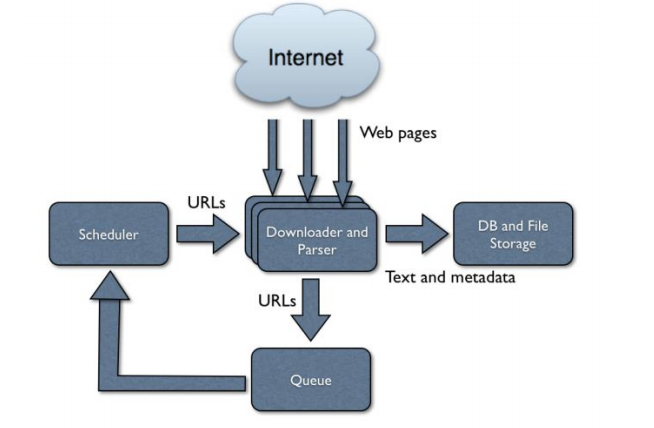
\includegraphics{pic/crawler-architecture.png}
\caption{网络爬虫架构}\label{fig:archetecture}
\end{figure}

\subsection{爬虫基本架构}\label{architecture}
前文介绍了不同的爬虫框架的各自的特点,但爬虫基本架构基本上是相同的。一个基本的爬虫架构如图\ref{fig:archetecture} 所示,主要包含了以下几个组件\cite{kausar2013web}:
\begin{itemize}
  \item Scheduler: 调度器,通过Scheduler决定哪些URL将要传入Downloader 进行下载,根据URL的优先级来调度URL请求的发布。
  \item Queue: URL队列,存储着待爬取URL,在爬虫初始化时初始化该队列。
  \item Downloader: 下载器,从网络环境中下载HTML页面。
  \item Parser: 对网络页面进行解析,包括所需要的结构化数据以及页面中的超链接,然后根据相关算法对链接进行筛选,最后倒入到URL队列中。
  \item Storage: 数据存储,将已经解析好的结构化或者半结构化数据进行处理,数据持久化,以便后续处理。
\end{itemize}

\subsection{爬虫基本流程}
一个爬虫基本的爬取流程\cite{wikipedia_web_crawler},便是从一个初始的URL集合出发,下载URL对应的页面;并对页面内容进行解析,
提取出相应的页面元素,以及页面上的链接;然后对页面链接进行过滤操作,获取所需要追踪的链接,将提取出的新链接放到任务队列中去;最后
直到队列中没有新的链接,爬虫便会结束。其中网页内容的解析、链接跟进策略以及链接过滤是爬虫能够爬取目标数据的关键。在实际的爬取
场景中,爬虫爬取的网站可能会存在动态页面加载的问题,给爬虫的爬取带来一定的困难。另外,大型网站往往还会设置一定的反爬策略来
限制爬虫机器人的爬取,这时便需要为爬虫配置相应的反反爬策略来绕过网站的限制。



\subsubsection{网页解析:XPath和CSS选择器}\label{page_parser}
网页数据的解析,即对下载器下载的HTML文件中的数据进行提取,需要网页元素的定位与匹配。
% 网络元素的匹配,我们可以直接考虑正则表达式来进行数据匹配,但这样匹配的效率很低,每次都需要全文匹配,代价很大,同时并没有利用到HTML文件的
% 结构性特点。
通常爬虫都是采用XPath或者是CSS选择器来对页面进行解析\cite{panum2019kraaler}。

Xpath即XML Path,表示XML文档的路径,是一种用来识别XML文档元素的查询语言\cite{grigalis2014using}。
爬虫能够通过Xpath表达式来寻找文档中的特定节点,Xpath会根据XML树状结构,提供在数据结构树中寻找节点的能力。由于Xpath的这一特性,爬虫可以
一层一层地遍历XML结构树,相较于CSS选择器,Xpath更加灵活,它能够在XML树中任一节点的任一方向进行搜索,例如探寻该节点的父辈节点或是查找具有某些属性
的子节点。大部分HTML页面都通过层叠样式表来设置网页样式,而这个层叠样式表就是CSS,它是一种样式表语言,用来描述HTML或是XML文档。
CSS选择器相比于Xpath,它能更快地找到对应元素,可读性较好。

\subsubsection{链接跟进策略}
爬虫爬取过程中,后续链接的提取是问题的关键,它决定了爬虫爬取的方向\cite{mendelzon1997querying}。

广度优先搜索策略是最常见的做法,它会维护一个先进先出队列,每次都把将要爬取的链接入队,并且按照链接提取的顺序进行链接的爬取。该策略属于盲目搜索策略,不会考虑当前搜索位置,
会遍历整个网站,通常会爬取到一些无用的页面,效率较低。

深度优先搜索策略则是从种子页出发,一个链接一个链接的跟进,直到该链路已经没有了后续链接,则结束该链路的爬取,进行回溯,从上一级页面开始爬取。该策略
无法保证链接提取的顺序和爬取顺序一致,同时如果没有限定爬取深度,可能会陷入到有着无穷后续链接的链路。

启发式的最佳优先搜索算法,基于某种估计、分数或者是优先级来选取最合适的链接进行跟进。最有名的便是fish-search算法\cite{de1994searching},该算法基于相关文档会包含更多相关文档的链接的
假设,维护一个URL列表,通过Depth、Width和 potential\_score参数来表示网页的深度、每页最多爬取的链接数以及网页相关度,根据potential\_score来动态改变URL在列表中的
位置,将优先级更高的URL排在列表前列,先进行爬取。该算法能够改变传统策略中按照URL出现次序依次爬取的机制,优先处理了对相关网页的爬取。

\subsubsection{链接过滤}\label{filter}
为了防止爬取到重复页面,爬虫需要考虑重复URL的识别。
爬虫实现重复URL过滤,可以通过内存对象存储所有的URL或者是嵌入式数据库\cite{singh2014review}(例如:Berkeley DB),每次提取到的新的链接时,需要查询内存对象或嵌入式数据库,查看是否已经重复,但这种方法内存消耗较大,随着爬取的URL数量的增加,内存压力会越来越大。
链接过滤可以通过将URL集合存储到外部数据库(例如Redis数据库)中,但这样会存在的一定的网络通信开销。
另外还可以通过布隆过滤器\cite{christensen2010new}(Bloom Filter)来检索URL是否在已爬取URL集合中,这种方法的空间效率和时间效率都要超过一般的算法,
但布隆过滤器存在一定的误报率,并且删除操作很困难。


\subsubsection{动态页面加载}\label{sec:page-load}
动态页面与静态页面相对应\cite{hand2014data},静态页面是指存在于服务器上的文件系统中的HTML文件,当用户通过浏览器访问相应的URL时,服务器会将HTML文件返回
给浏览器,浏览器再加以渲染呈现给用户,早期的网站通常都是些静态页面。

动态页面则与之不同,页面中的许多数据往往需要Ajax\footnote{https://en.wikipedia.org/wiki/Ajax\_(programming)}技术动态生成,并且许多数据并不会直接出现在HTML源代码中,需要经过浏览器渲染才会得到数据。页面上的元素
并不是一成不变的,浏览器会通过js调用异步通讯组件并使用格式化的数据来更新Web页面上的内容。对于这些需要js代码动态加载的数据,爬虫往往很难爬取。开源爬虫
框架采用的下载器下载的页面都是网页源代码,并未对js动态加载的数据进行渲染,需要相关工具能够对这些动态js页面进行渲染,这样才能使爬虫获取相应的数据。


\subsubsection{反爬策略与反反爬策略}
反爬是指网站通过一定的反制措施来干扰爬虫的正常运行,从而间接地起到网站防护的作用。反反爬则是爬虫通过绕过网站设置的反爬措施来获取所需要的数据。
如图\ref{fig:strategy} 所示,网站反爬策略以及爬虫的反反爬策略主要分为以下几种情况:
\begin{enumerate}
  \item User Agent检测:网站通过从请求的Header中获取User Agent进行检测是一种比较常见的方法,爬虫可以通过模拟User Agent的方式绕过。
  \item IP限制:限制IP访问次数,通过检测用户行为,如一定时间段内,IP访问请求次数过多,对IP加以限制。爬虫往往通过
  构造代理IP池,以及限制访问频率的方法加以绕过。
  \item Ajax页面动态加载:页面通过Ajax进行数据的动态加载,使得爬虫只能爬取页面源代码,无法获取所需要的数据。这种情况,爬虫往往通过
  一些工具模拟浏览器操作的方式绕过。
  \item 登录认证:网站设置某些数据的访问需要用户登录。爬虫通过模拟登录过程,获得Cookies,每次访问都带上Cookies进行网页爬取。
  \item 验证码识别:网站设置访问验证,需要用户手动验证来访问网页。爬虫通过OCR技术识别验证码,或者通过人工打码平台进行识别,甚至是手动验证。
\end{enumerate}


\begin{figure}[htbp]
\centering
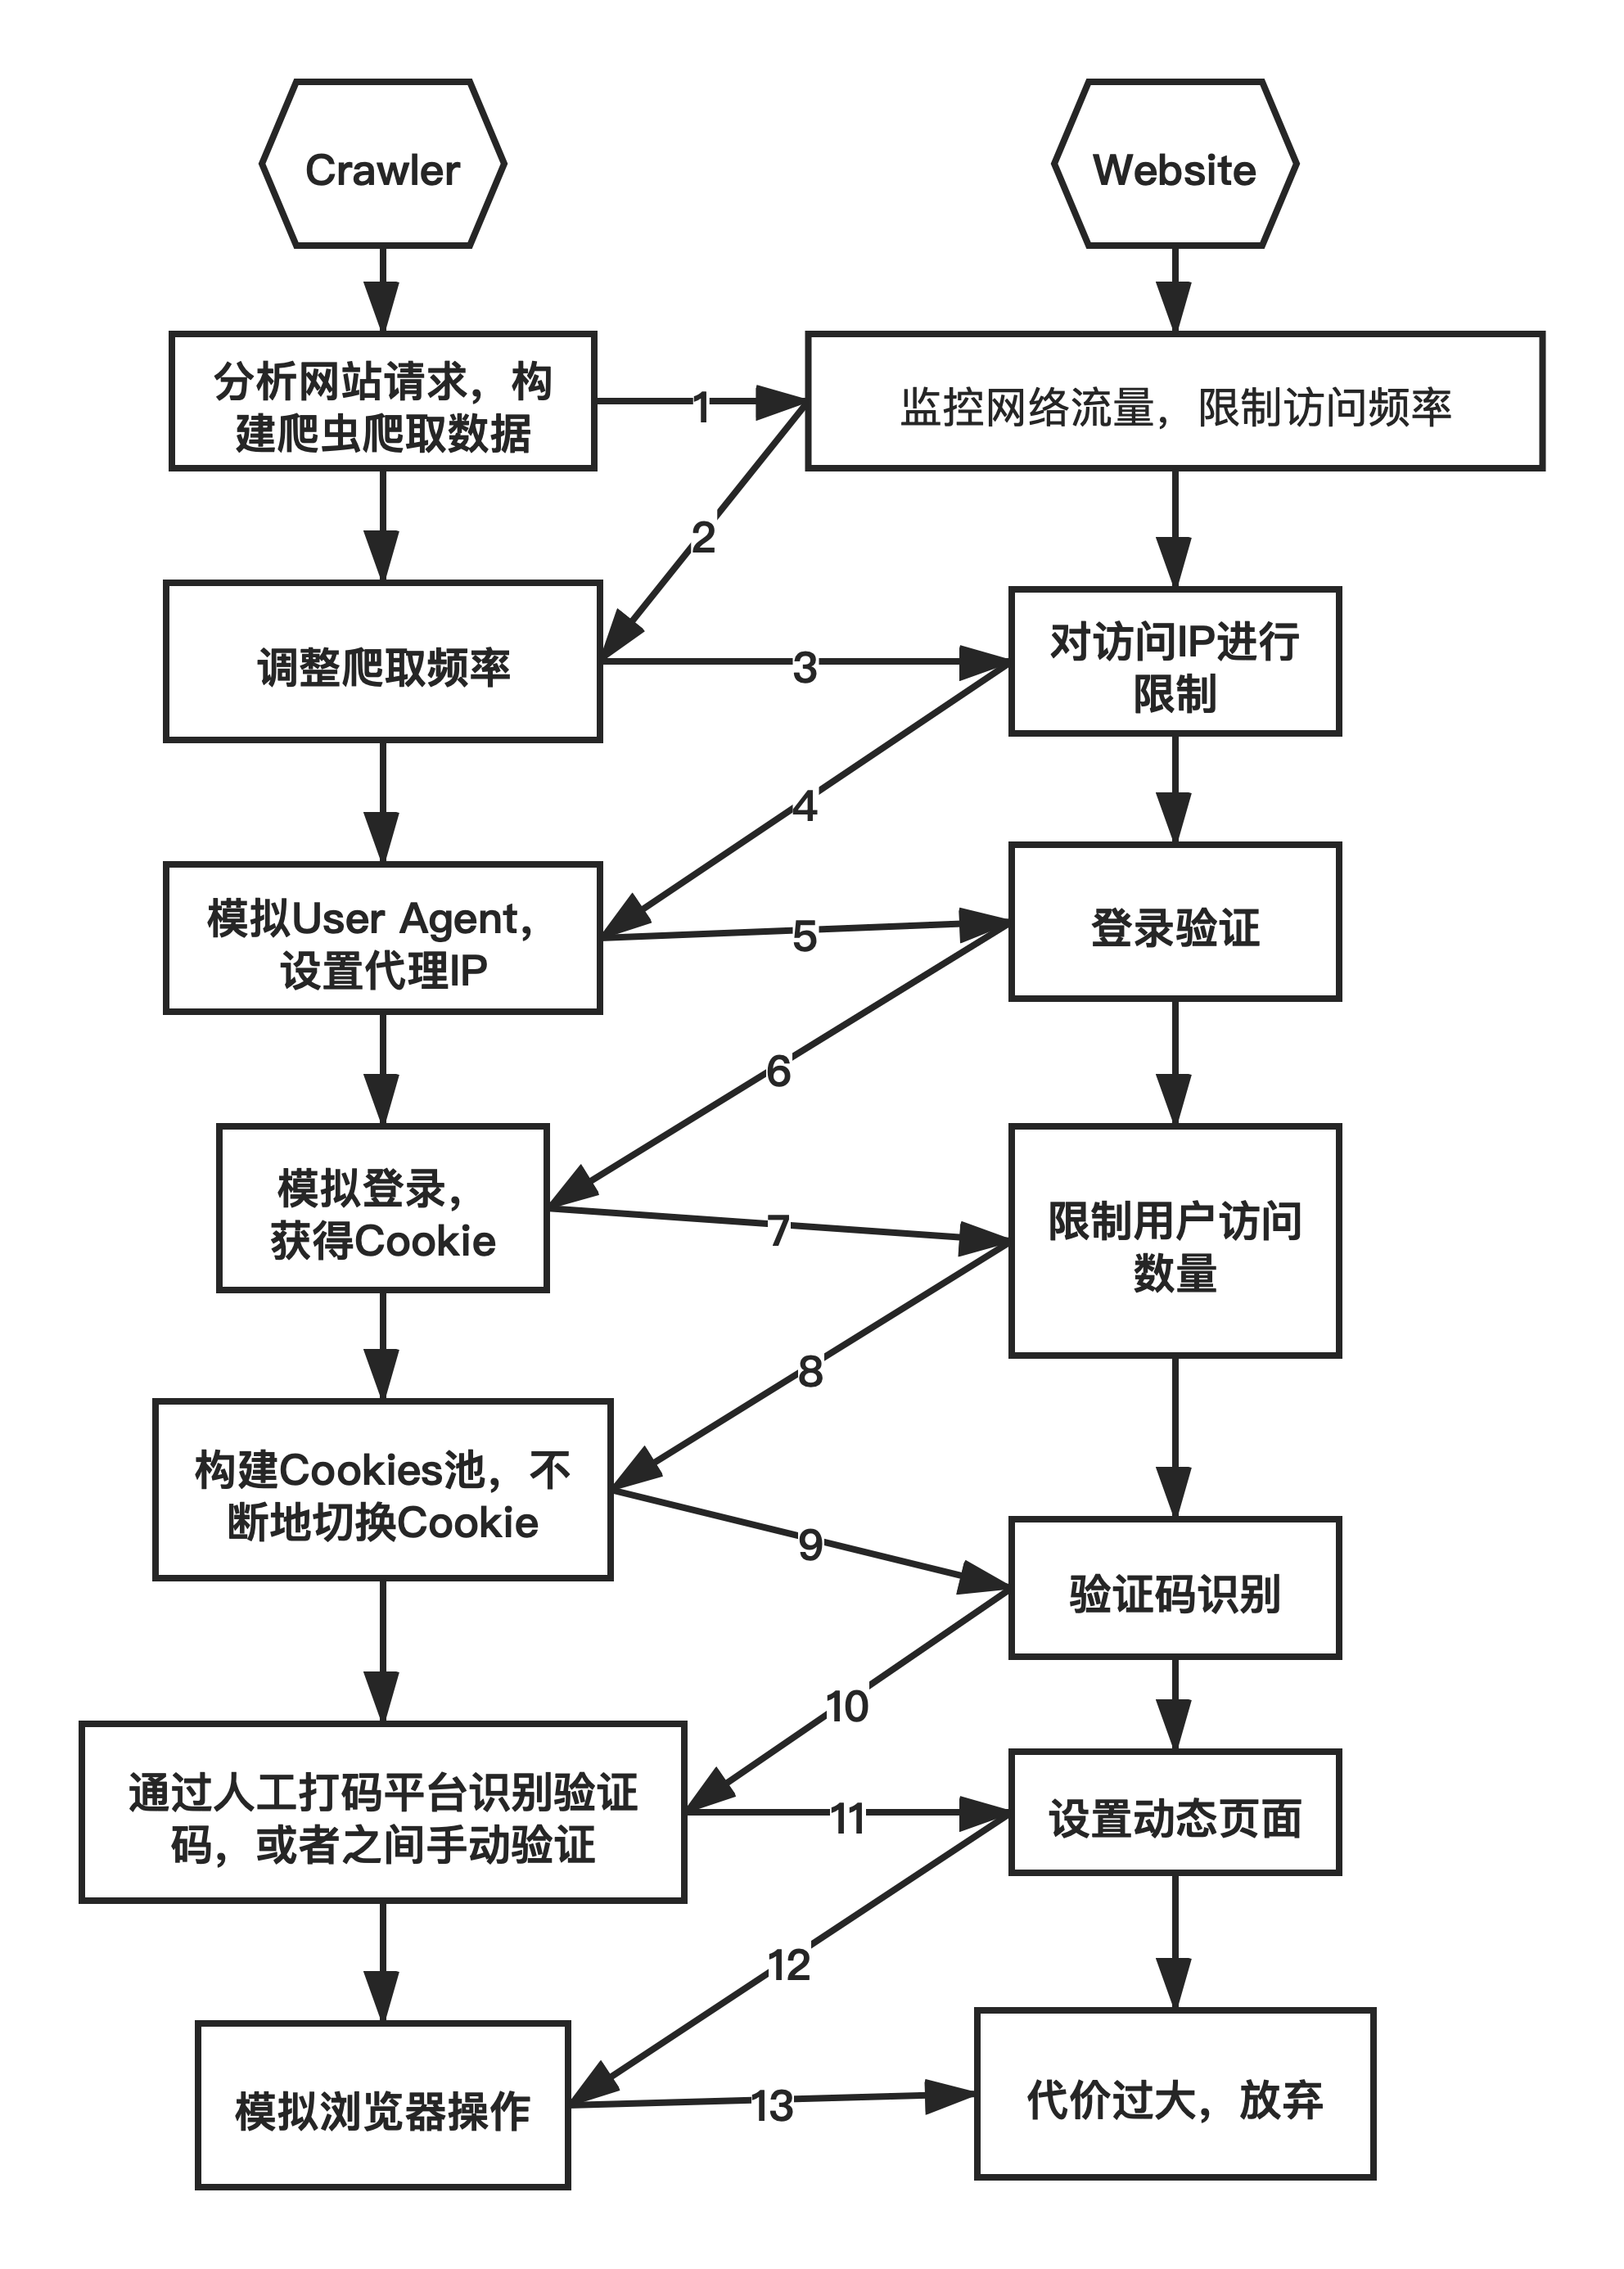
\includegraphics[width=0.8\textwidth]{pic/anti-strategy.png}
\caption{反爬策略与反反爬策略}\label{fig:strategy}
\end{figure}


\section{响应式编程}\label{reactive_programming}
响应式编程是基于异步数据流的编程范式,面向数据流和变化传播。响应式编程基于流式处理,可以把包含一堆
异步事件的组合用操作符给清楚的表示,将异步回调模式表示成了邻接节点的关系,能够对数据的传播流动的方向加以把握。

实际上Reactive Programming并不是一个新鲜的概念,它用来解决异步非阻塞编程中存在的问题。虽然异步编程可以通过回调函数来处理,
但是随着业务逻辑越来越复杂,回调函数这种模式会陷入到“回调地狱”的困境,而Java 8引入的CompletableFuture,虽然能够处理
异步事件的组合,但还是会存在各种各样的问题\cite{7203125}:
\begin{itemize}
  \item 对于Future对象的处理,往往容易陷入到一种阻塞的情景,依然需要调用阻塞的get方法。
  \item 不支持任务的延迟执行。
  \item 缺乏对多值属性的表示,另外还缺乏友好的异常处理机制。
  \item 难以优雅地实现异步任务的编排。
\end{itemize}


\subsection{响应式规范}
响应式编程的出现便是来解决异步编程中存在的问题,响应式编程需要遵守Reative Streams\cite{satyanarayan2015reactive}标准。Reactive Streams是响应式编程规范,如今已经被多个企业所采用,如Netflix、Oracle等。在Java 9之后,java.util.concurrent.Flow也支持了这个标准。

\begin{figure}[htbp]
\centering
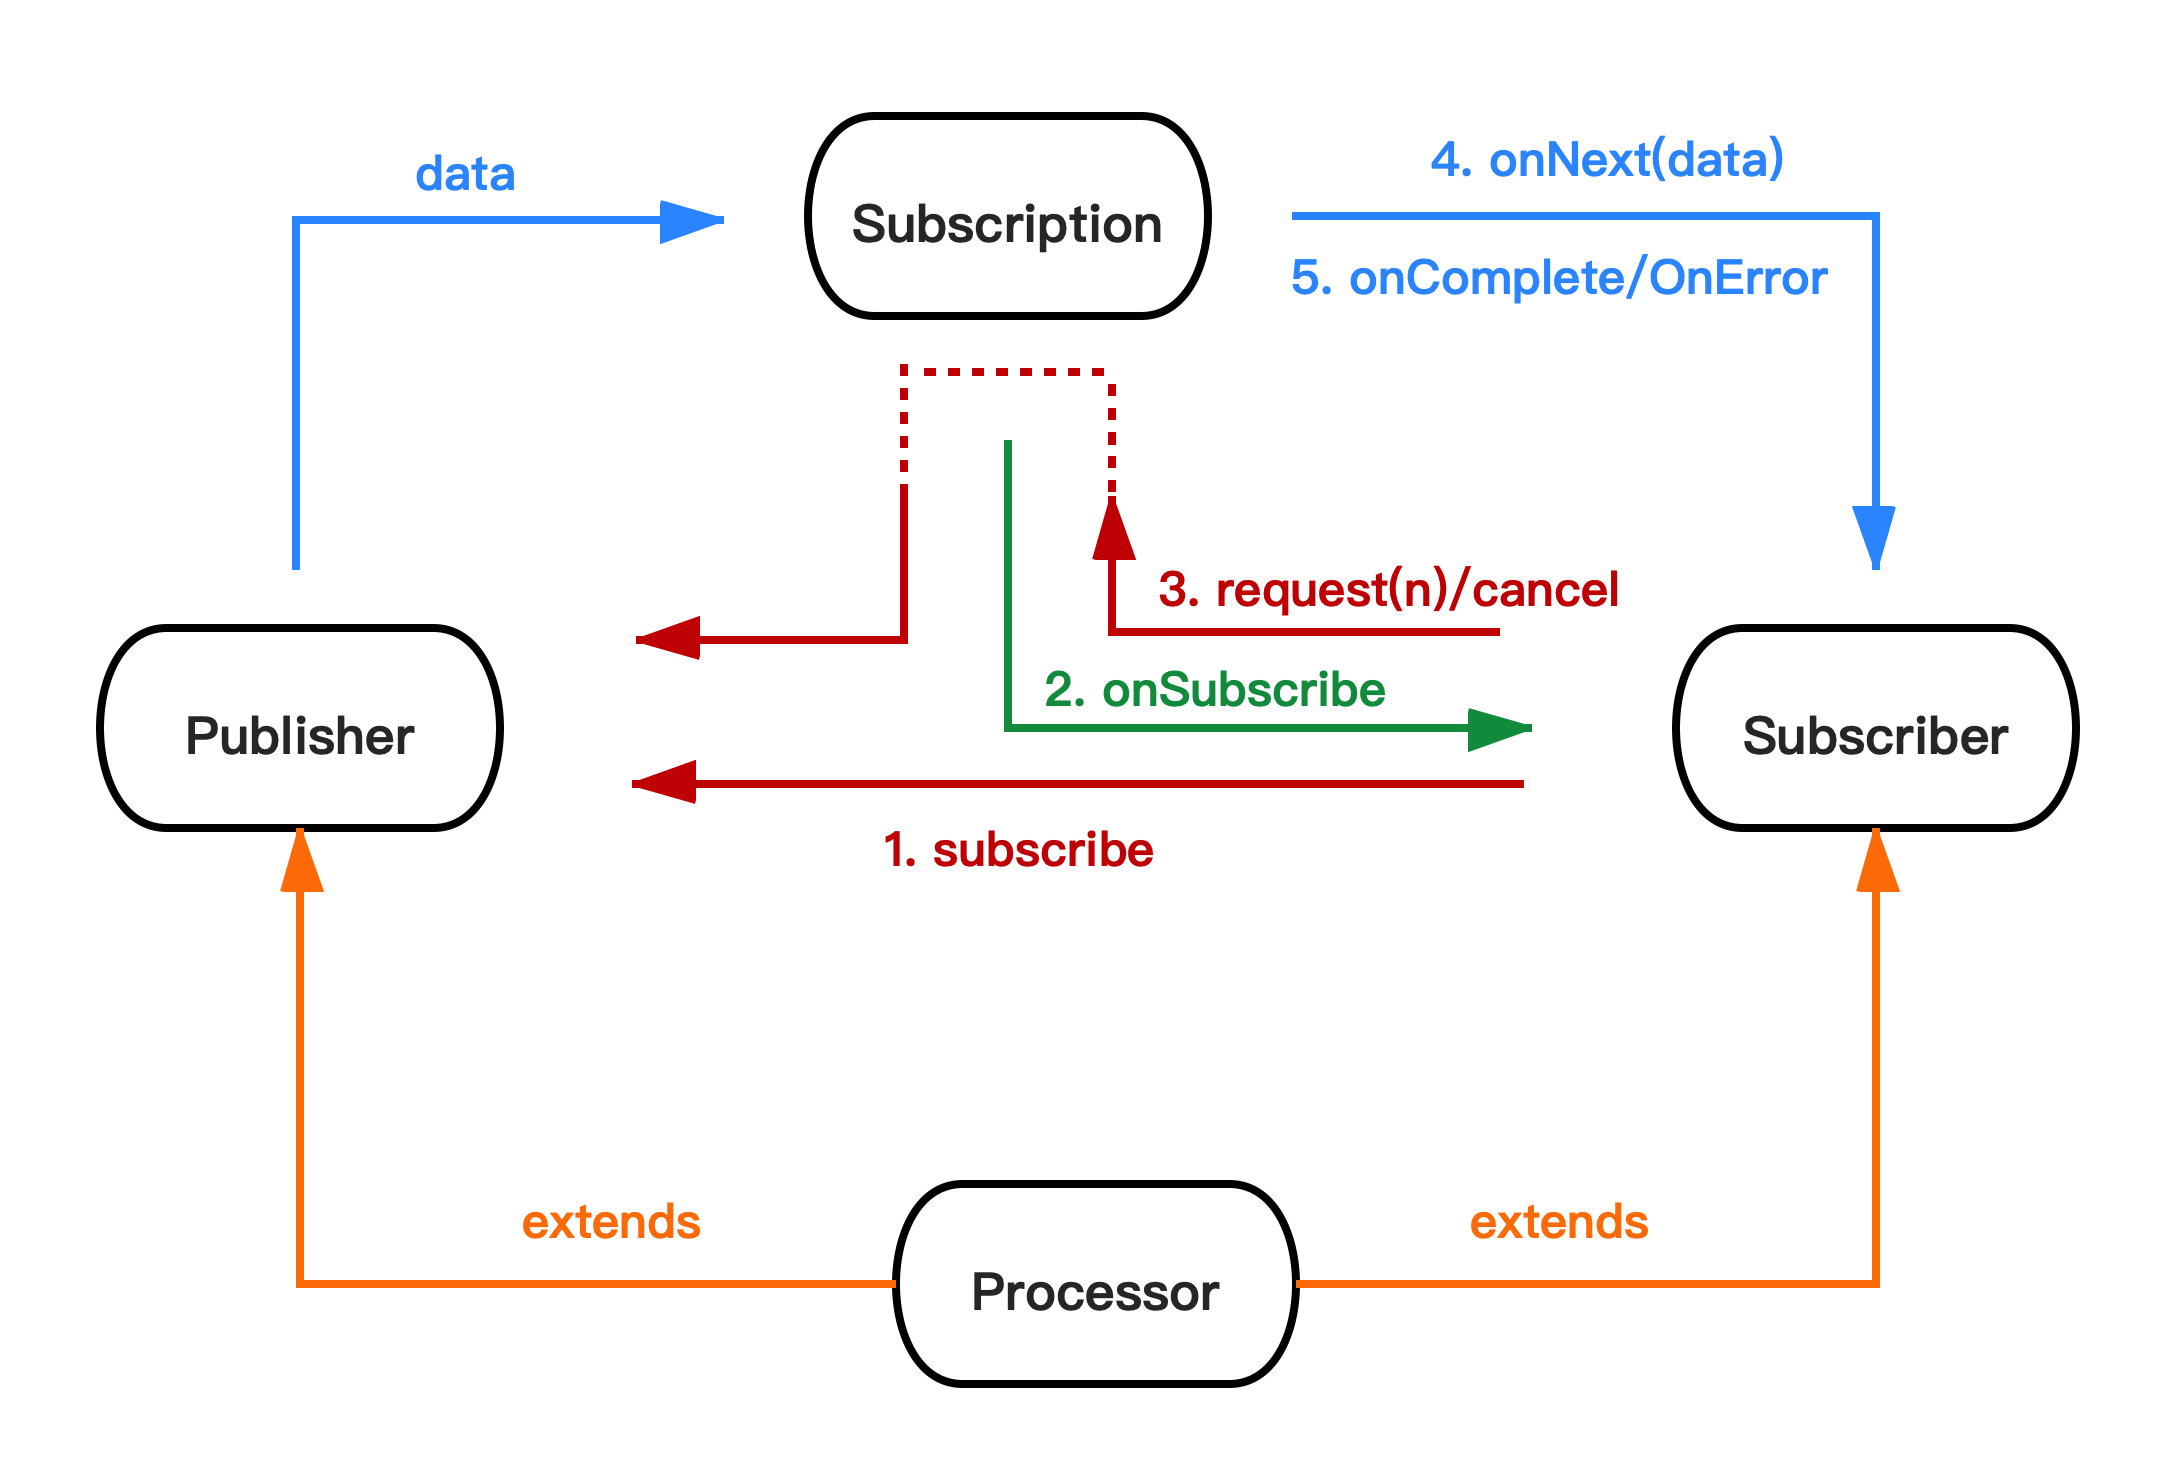
\includegraphics[width= 0.8\textwidth]{pic/reactive-streams.png}
\caption{Reactive Streams规范}\label{fig:reactive-stream}
\end{figure}

Reactive Streams的目的在于通过流处理机制提供一个异步数据处理序列\cite{7203125}。
如图\ref{fig:reactive-stream} 所示,它需要实现4个接口,来管理跨异步边界的流式数据交互,即将数据在线程池中传递,同时还要确保接收方不需要强制
缓存任意数量的来自发布方的数据。换而言之,需要实现背压机制,线程之间的缓冲队列是有界限的。

4个接口如下所示:
\begin{itemize}
  \item Publisher: 数据源,发布0到N个信号,其中N可以是无限的。另外它还可以提高两个终止事件:error 和 completion。
  \item Subscriber: 和数据源对应,是数据消费者,可以消费从0到N个信号,N可以是无限的。Subscriber会在初始化的时候
  接收一个Subscription对象,通过它来请求要消费的数据。
  \item Subscription: Subscriber初始化的时候创建,它来控制下一步消费多少数据以及何时停止消费。
  \item Processor: 既可作为数据源,也可以作为消费者。
\end{itemize}


\subsection{响应式系统}

随着计算机软件技术的发展,应用程序的需求与原来相比已经发生了巨大的改变,之前一个大型应用程序只需要跑在数十台服务器上,要求秒级的
响应时间\cite{6691765}。然而,现在的用户希望能够达到毫秒级别的响应,以及系统能够处理PB级的数据量,之前的软件架构已经无法满足当前的需求。
人们需要一套贯通整个系统的架构设计方案,系统需要能更加的灵活,系统的开发和调整也能够变得更加容易;
同时系统必须松耦合,系统组件容器被及时替换;另外还必须具备可伸缩的特性,能够水平的扩展应对高负载情况。
总结来说,系统必须具有存在着这样的特质\cite{fionda2015nautilod};

\begin{itemize}
  \item 即时响应性(Responsive):只要有可能,系统就会及时地作出反应。即时响应意味着系统专注于提供快速且一致的响应时间,确定可靠的反馈上限,从而
  提供稳定的服务质量。
  \item 回弹性(Resilient):回弹性意味着即使系统出现了异常或者是失败,仍然能够保持即时响应性,这能确保系统的高可用。而回弹性的实现,是通过复制,
  隔离和委托来实现。对于一个响应式系统而言,组件与组件之间的隔离,抑制失败在组件间的传播,使得系统部分的失败无法影响到系统整体,并且
  能够独立恢复。
  \item 弹性(Elastic):系统能够根据工作负载做出反应,调整相应的资源配置来保证系统的即时响应性。换句话说,系统能够根据负载进行自动扩展。
  \item 消息驱动(Message-driven):系统依赖与异步的消息驱动,通过异步的消息来实现系统各个组件之间的松耦合关系,给组件明确的边界。并通过回压等手段,使得
  系统实现负载管理以及流量控制。
\end{itemize}

% \begin{figure}[htbp]
% \centering
% \includegraphics[width= 1\textwidth]{reactive-system.png}
% \caption{响应式系统}\label{fig:reactive-system}
% \end{figure}




\section{本章小结}
本章首先对爬虫进行了介绍,阐述了三种类型的网络爬虫,分别是通用爬虫、聚焦爬虫以及垂直爬虫,并对爬虫涉及的相关背景技术作了简要介绍。
本章还介绍响应式编程相关内容,包括响应式编程范式基本概念,响应式规范以及响应式系统。

下一章将对本文提出的异步流式爬虫框架进行详细介绍。

%%%%%%%%%%%%%%%%%%%%%%%%%%%%%%%%%%%%%%%%
%%%%%%%%%%%%%%%%%%%%%%%%%%%%%%%%%%%%%%%%
\chapter{异步流式爬虫框架}\label{Chapter_reflect}
% 本章系统设计介绍了爬虫数据模型与网站结构的映射和爬虫爬取模型的构建。
% 爬虫数据模型定义部分,从Web页面结构和网站的逻辑结构出发,基于网站树形逻辑结构,提出了一种层次树模型统一描述网站结构,接着
% 介绍了层次树模型和对象数据模型之间的映射关系。接着介绍了异于传统爬虫的流式爬取模型的构建和使用场景。
本章首先介绍了传统爬虫的编程模型,分析了传统编程模型的利弊,并在此基础上,提出了一种异步流式的响应式爬虫编程模型。


\section{传统爬虫编程模型}
传统爬虫编程模型主要有三类,第一类多线程爬虫编程模型,爬虫内部通过线程池来实现并发爬取;第二类是单线程事件循环爬虫编程模型,爬取主流程是跑在单个线程上的,IO操作通过事件循环
异步执行;第三类则是分布式爬虫模型\cite{boldi2004ubicrawler},爬虫主要借助于Hadoop、Storm等大数据平台,通过平台提供的组件进行爬虫的组装。

\subsection{多线程爬虫编程模型}
多线程爬虫是最常见的爬虫场景,目前大部分的开源框架都是采用的多线程的爬虫模式。例如Webmagic框架便是采用的多线程模型进行爬取,通过配置相应的线程池来处理每一个爬虫请求。
相比于其他编程模型而言,多线程实现比较简单。



\begin{figure}[htbp]
\centering
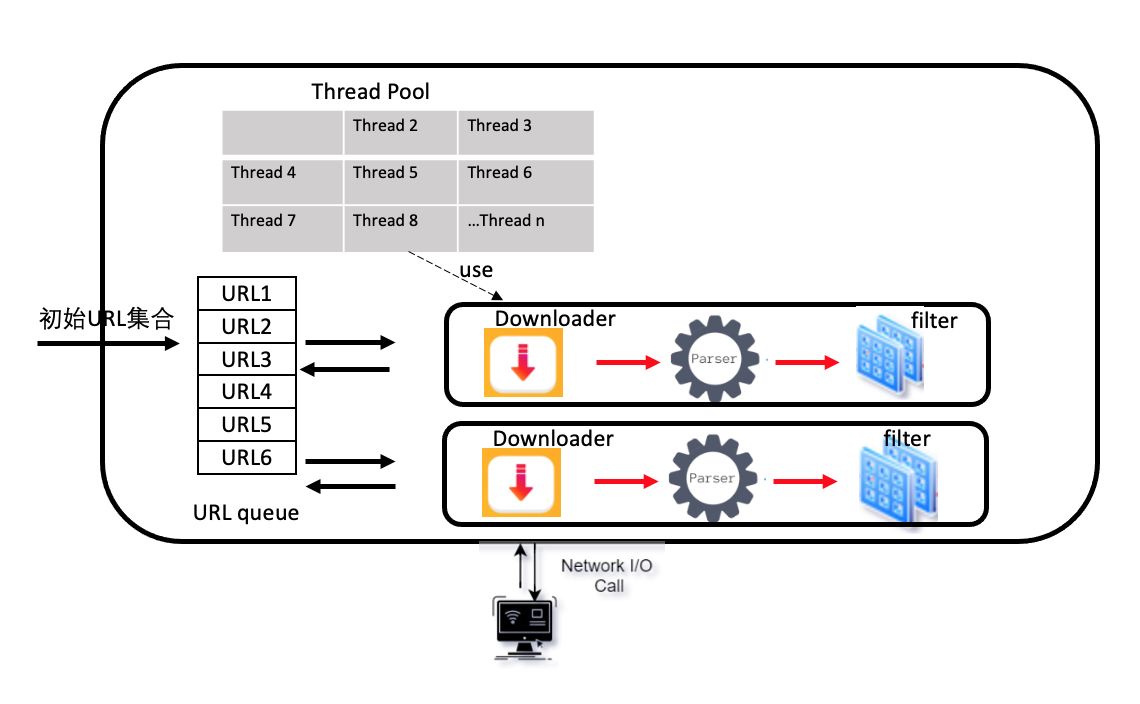
\includegraphics[width= 0.98\textwidth]{pic/thread_pool.png}
\caption{传统爬虫多线程模型}\label{fig:threadpool}
\end{figure}
传统多线程模型如图\ref{fig:threadpool} 所示,使用同步编程模型,每一个URL请求都对应一个线程处理\cite{rheinlander2016potential}。该线程负责页面的下载、解析、链接过滤等操作,
在下载阶段,会进行相应的网络IO操作,需要从网站获取Response,此时请求线程必须同步等待以获得响应。在这种情况下,线程处于等待状态,CPU空闲,所以
该模式会采用一个线程池来处理,目的就是当有线程处于等待状态时,能够通过线程的调度,让已经就绪的线程调度执行,充分利用CPU的计算资源。线程池模式
对于单位时间内请求量较少的爬虫程序来说是可以接受的,但是对于单位时间内请求量大的爬虫而言,线程池编程模型最终会让爬虫程序变慢或者是请求无法得到响应。
这种全链路线程池处理模式,当并发量逐渐增大时,会使得线程间的调度开销增大,同时由于CPU资源短缺,可能会使得已经就绪的线程得不到及时的调度。

多线程爬虫编程模型,其优点是编码简单、能够提高响应速度、在多CPU的环境下能够体现多核的优势。对于请求量不大的爬虫来说,多线程模型是可以接受的。
但在负载大的情况下,该编程模型会消耗大量的内存,因为每个爬虫请求都要维护一个线程堆栈。另外持续的上下文切换也会导致大量的CPU时间损失。
由此产生的间接影响便是CPU高速缓存未命中的概率增加,减少线程池的绝对数量可以提高单个线程的性能,但是限制了爬虫请求的可伸缩性。



\subsection{单线程事件循环爬虫编程模型}
对于单线程事件循环爬虫编程模型\cite{singh2014web},主线程执行事件循环,通过线程池来执行异步任务,通过事件循环和线程池来实现异步IO。例如Scrapy爬虫,它通过
Twisted异步通信框架来实现事件循环,Scrapy框架向开发者
屏蔽了底层编程模型的细节,将回调函数暴露给开发者来编写页面解析逻辑。

如图\ref{fig:singlemodel} 所示,该模型下,爬虫通过一个请求队列来缓存到达的每一个请求,通过一个主线程的事件循环不断地处理请求以及回调事件。每一个到达的请求的阻塞网络IO操作放在线程池中异步执行,并
注册回调函数,当阻塞任务执行完成后,会触发事件,在主线程中调用非阻塞的回调函数。爬虫主线程一直处理非阻塞的页面解析代码,而通过线程池异步执行网页下载请求。

\begin{figure}[htbp]
\centering
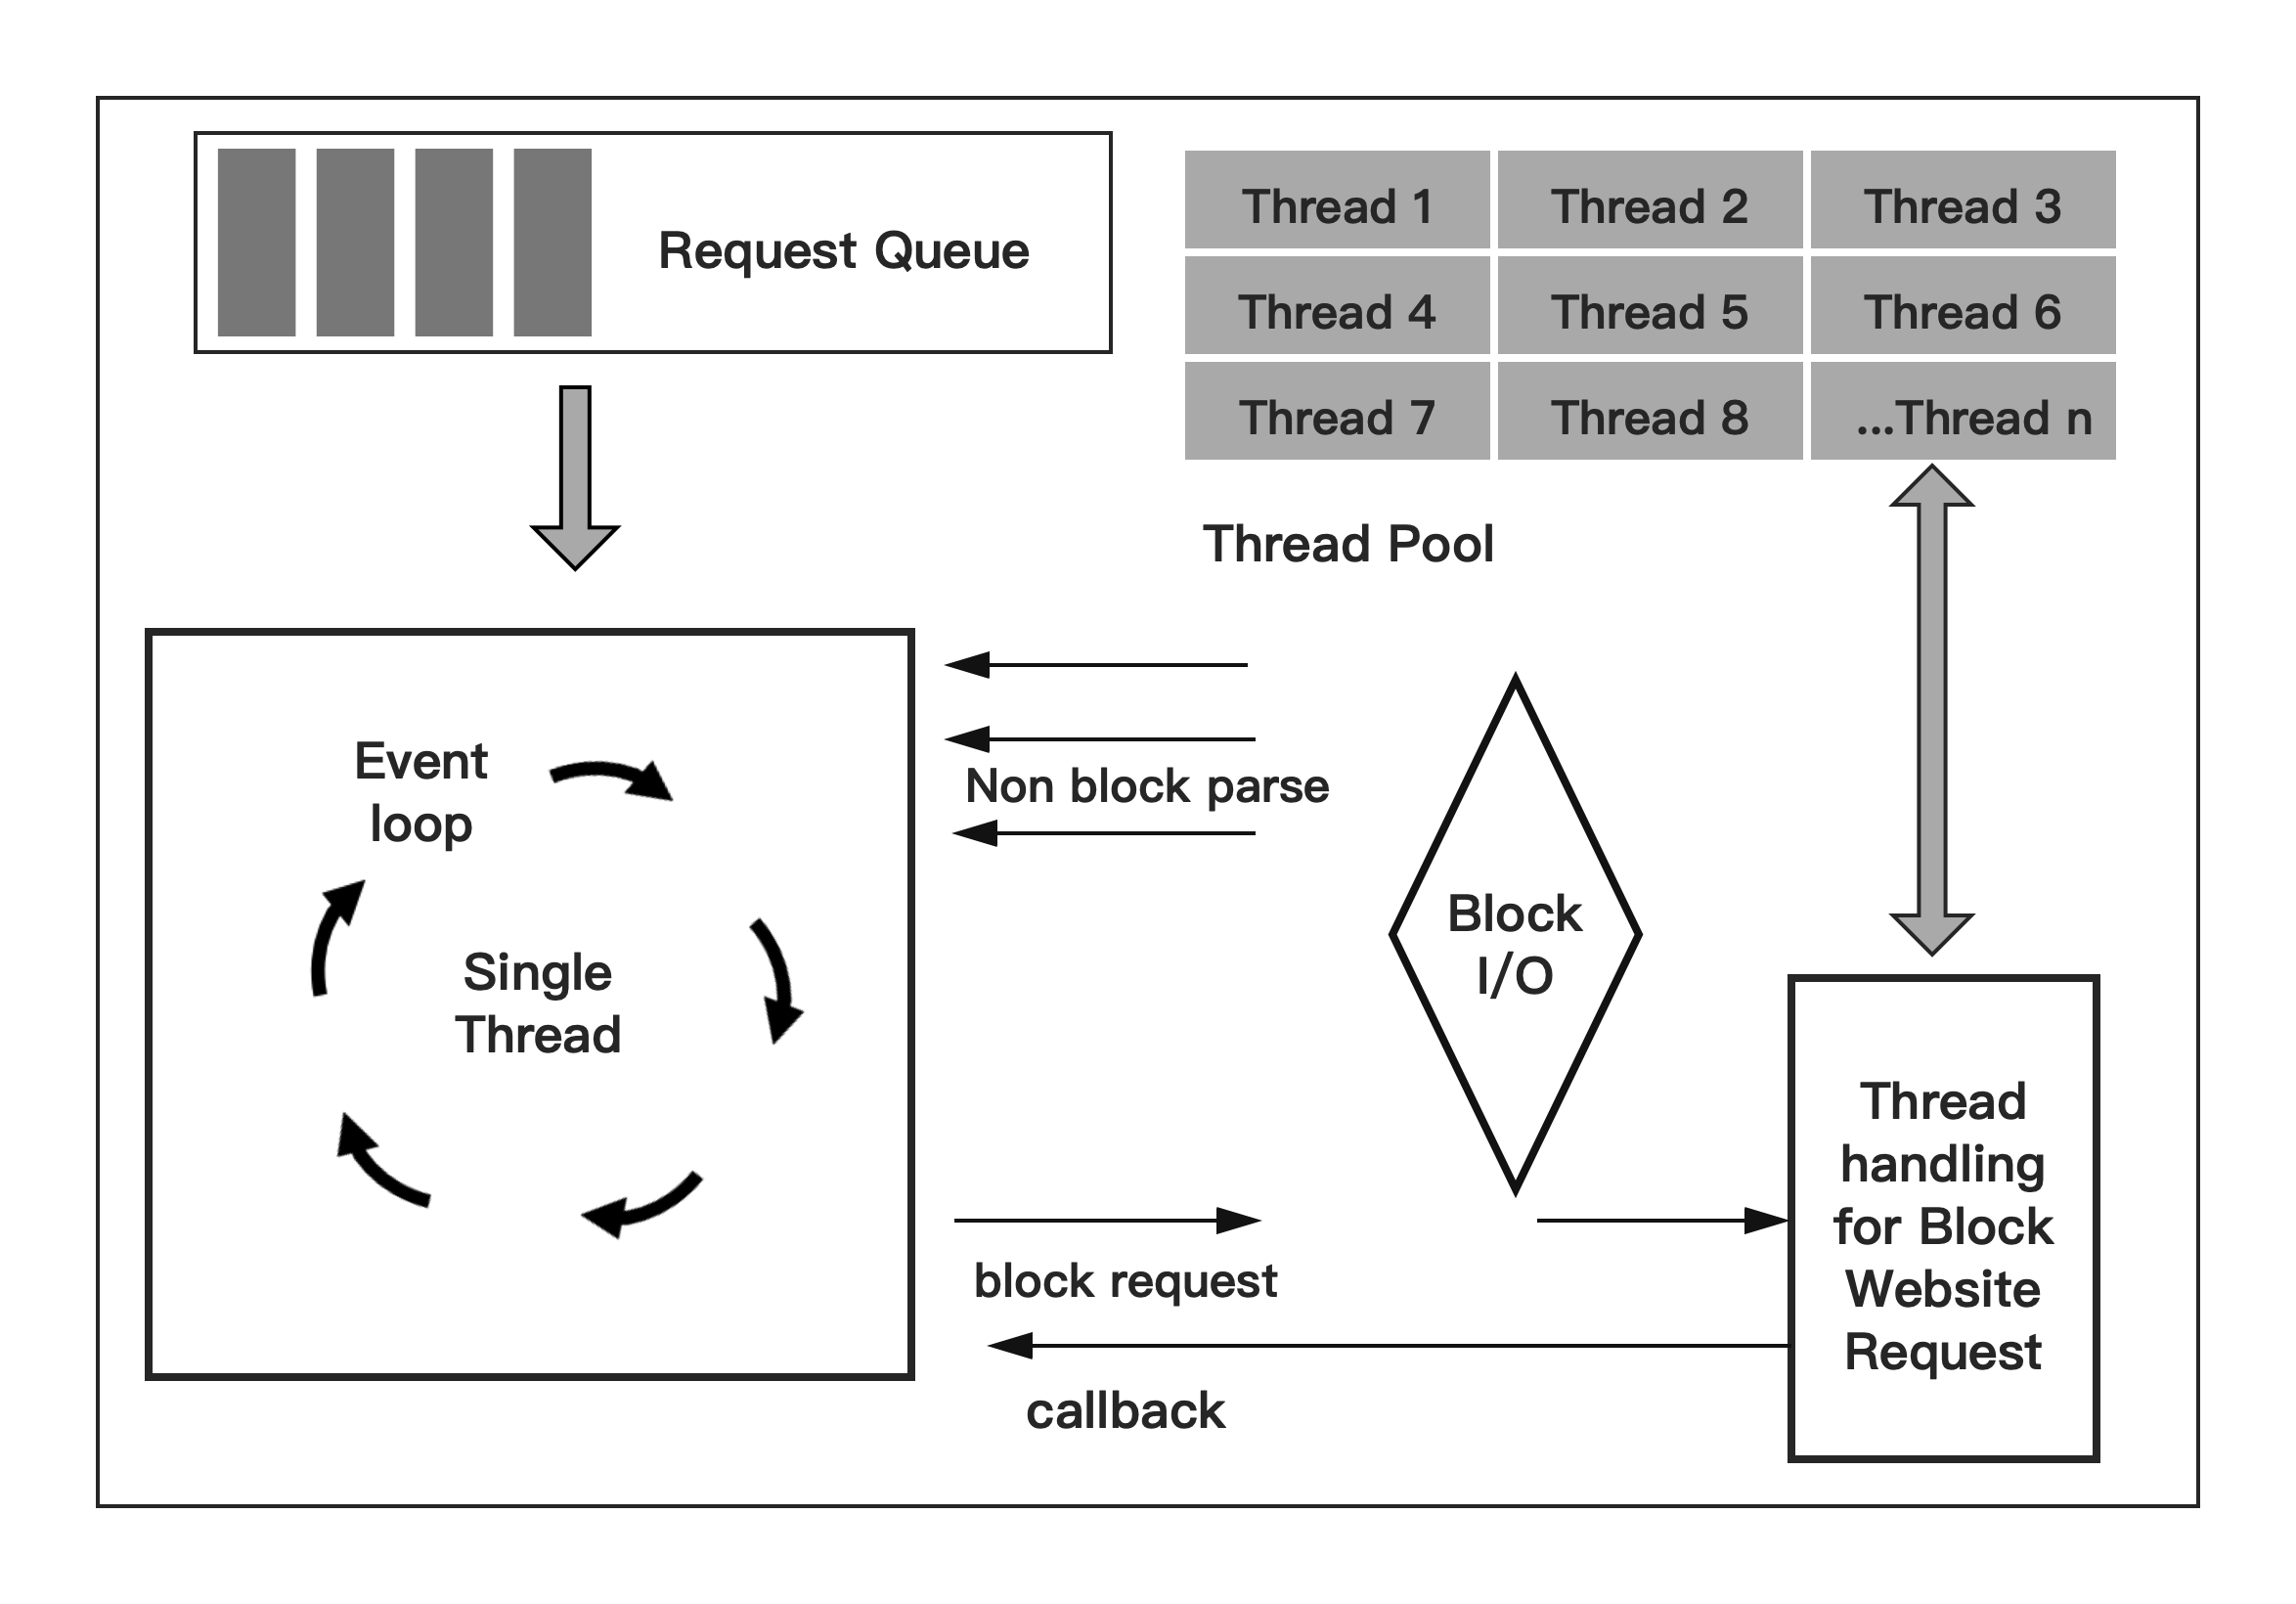
\includegraphics[width= 0.98\textwidth]{pic/model.png}
\caption{单线程事件循环爬虫编程模型}\label{fig:singlemodel}
\end{figure}


该模型的优势能够处理许多并发的爬虫请求,使用了较少的线程,CPU以及内存资源使用较少,同时避免了多线程死锁以及状态同步的问题。
在单CPU环境下,该模式会优于多线程模型,请求处理速度比多线程模型快,因为没有线程间的上下文切换以及加锁的开销。
但单线程模式无法利用CPU多核的优势,同时需要保证回调函数中不存在阻塞操作,不然会使得主线程处于阻塞的状态,无法处理其他请求。另外异常处理存在问题,
异步事件处理过程中产生的Exception并不能被主线程感知并处理。


\subsection{分布式爬虫模型}
% 分布式场景下的爬虫往往借助于大数据平台或是流式计算平台来实现。

如图\ref{fig:distributed} 所示,其中一台机器是master节点,并连接到多台工作节点上。master节点会维护一个中心队列来存储待爬取到URL列表,
master会将URL根据一定的策略分发到各个worker节点;worker节点进行网页爬取、链接提取以及数据解析等基本流程;然后将提取出来的链接以及解析的数据
给传输到中心节点master上;master节点对所爬取到数据进行汇总,然后将数据存储到数据库中\cite{brin1998anatomy}。

分布式爬虫模型能够将任务的生成和数据的抓取两个过程分开,master节点负责任务的分发和数据的收集工作,worker节点负责数据的抓取,能够通过水平
扩展worker节点的数量来提高爬虫的吞吐量,提高系统的可用性。但大部分的分布式爬虫都仅仅是维护一个全局URL队列,通过该队列来调度各个worker节点的
爬取任务,并没有对爬虫各个组件分别管理,没有充分利用分布式系统的特性,只是简单的爬虫实例的堆叠,无法充分利用各节点的资源。
% \begin{figure}[htbp]
% \centering
% 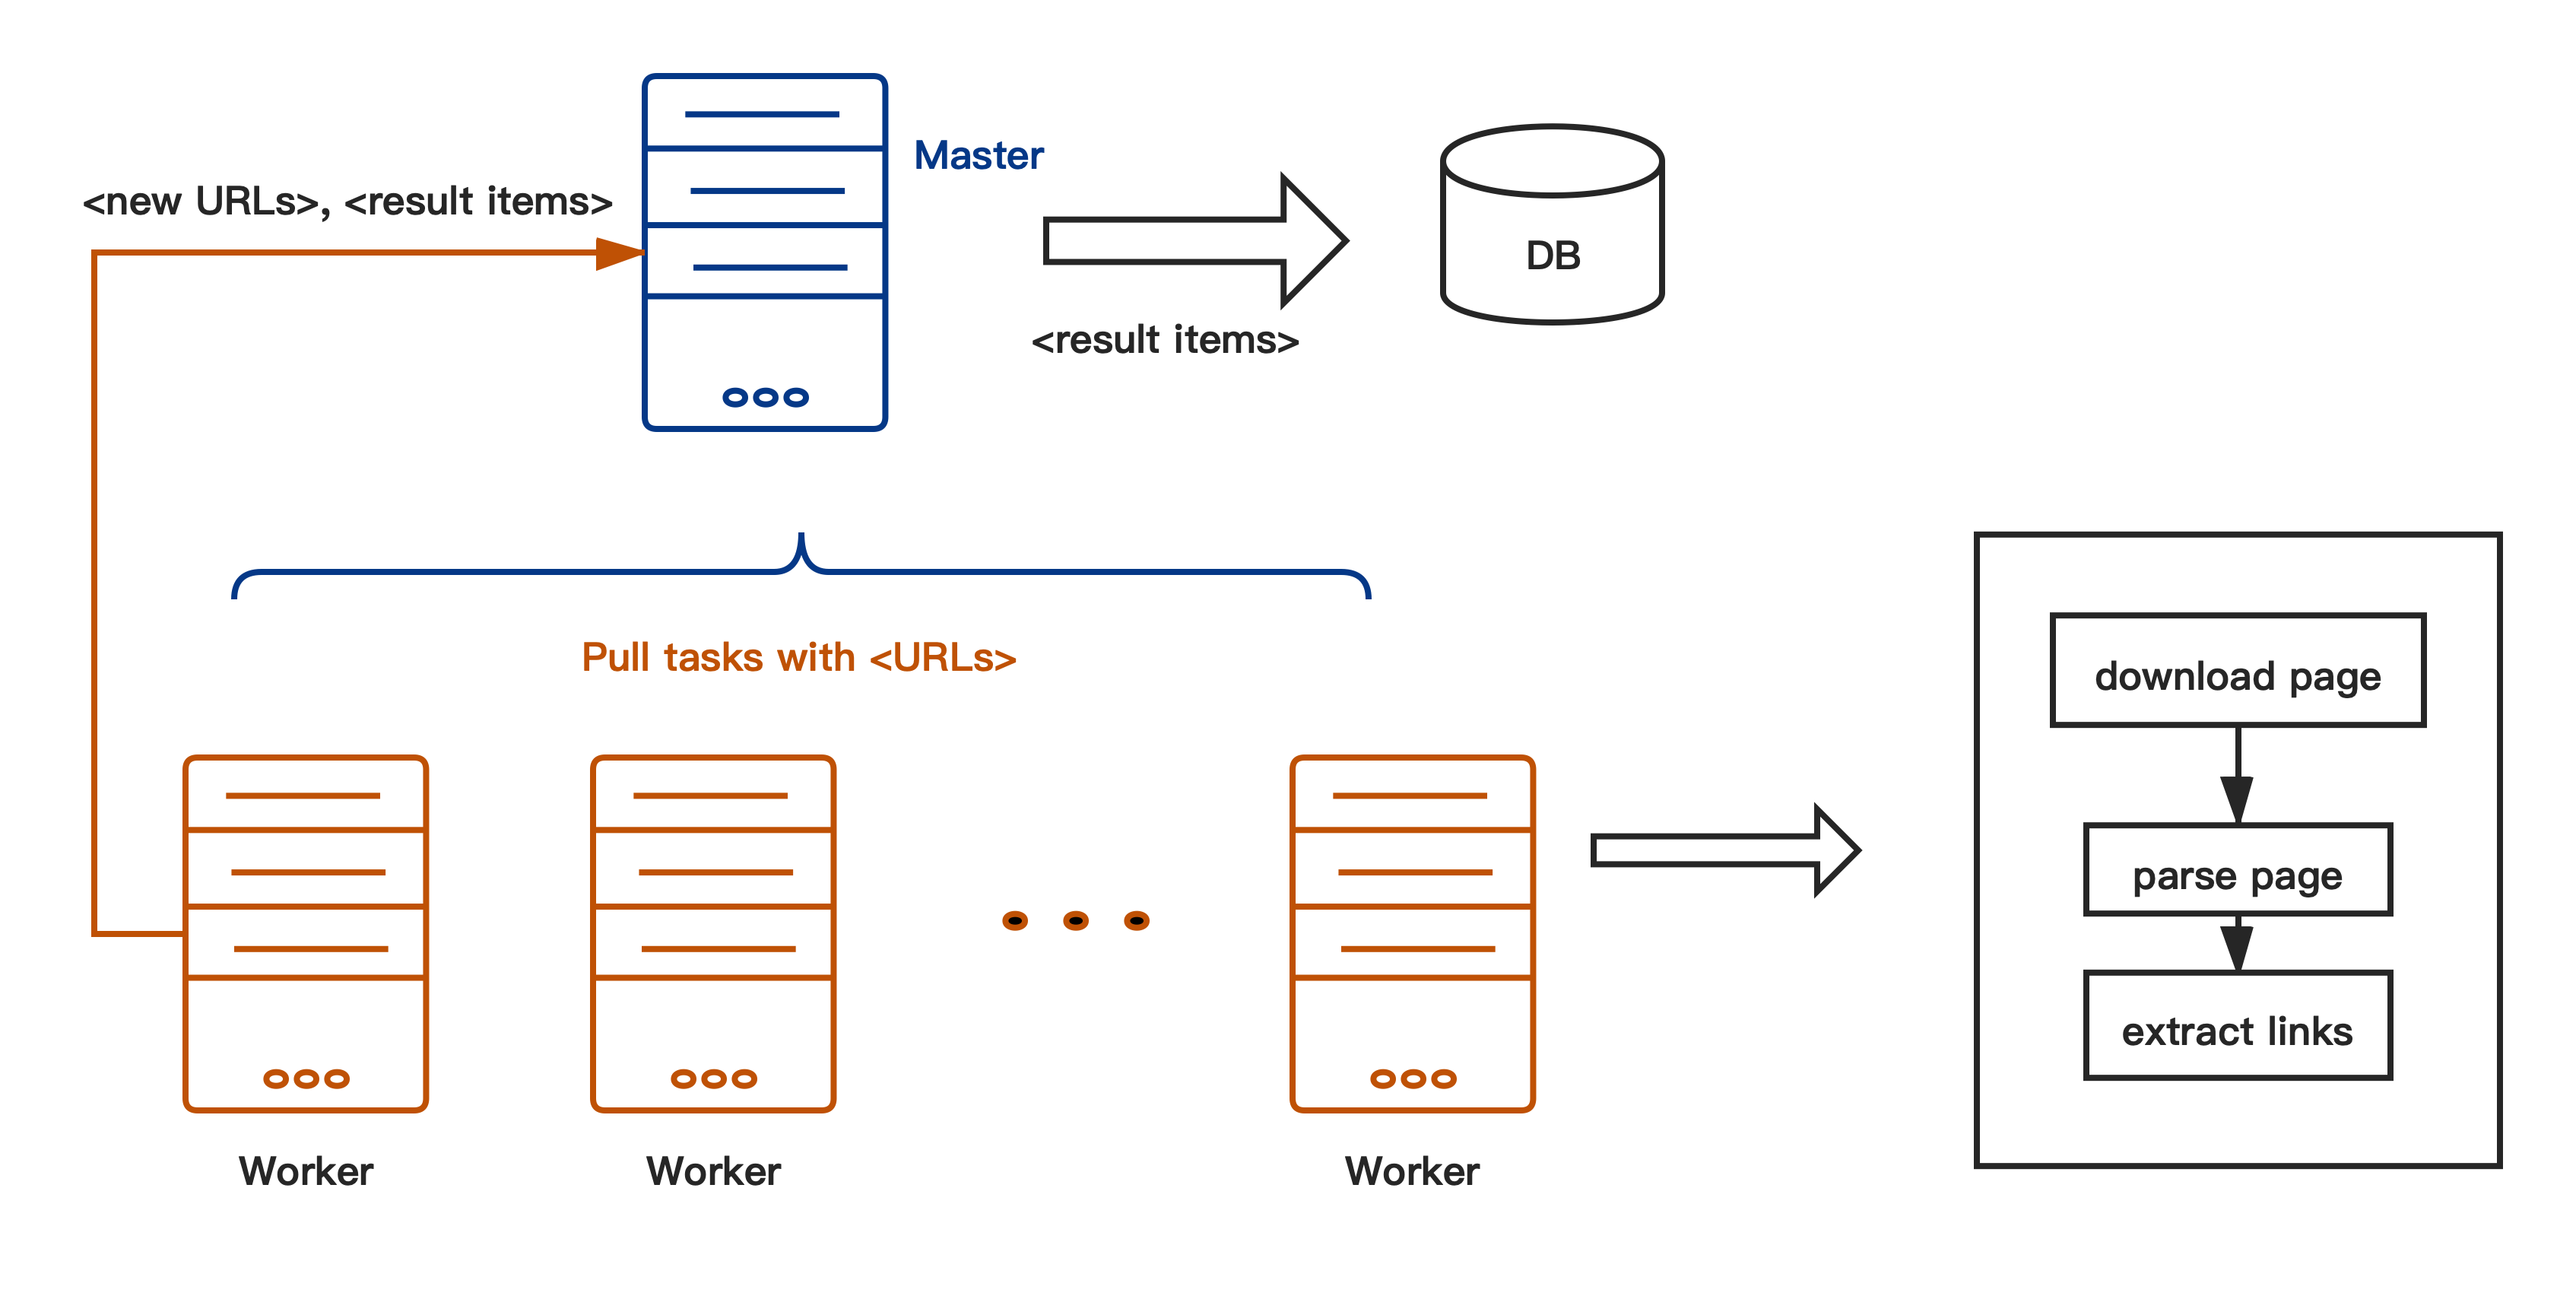
\includegraphics[width= 0.98\textwidth]{distributed.png}
% \caption{分布式爬虫模型}\label{fig:distributed}
% \end{figure}



\section{响应式爬虫编程模型}
上述的各种爬虫编程模型都有其各自的应用场景:多线程爬虫适合于爬取网页较少的网站,这样能充分利用多线程的优势,但不至于造成太多额外的CPU开销;
单线程事件驱动爬虫适合于爬取一些解析逻辑比较简单的网站,这样避免复杂的异常处理操作;
分布式爬虫适合于爬取大型的网站,但爬虫的构建比较繁琐。
不同编程模型都有其各自的特性,但都有一定的局限性。主要是三个方面:无法充分利用CPU资源;爬虫的编写不够简练;缺乏相应的异常处理机制。

对于这样的情况,Reactive Programming有很好的解决方案。考虑爬虫爬取过程中,网页下载以及页面解析阶段存在大量的耗时操作,
参考流式计算的思想,本文基于响应式编程,构造了一个响应式爬虫编程模型。
% 传统多线程模式每个线程只能处理一个URL请求,而且还必须等待请求的响应。而单线程事件循环模型必须在主线程维护一个事件循环,
% 这里我们通过一个线程请求网络数据,不等待响应的到来,而是设置一个回调函数,这个函数会等阻塞任务完成后自动执行。这样线程不必一直等待,可以继续处理URL队列中
% 其他请求。基于这样的考虑我们设计了响应式爬虫模式,如图\ref{fig:model}所示

如图\ref{fig:crawler} 所示,爬虫爬取呈现出流式的结构,先从Seed Urls开始,数据流经第一个组件,该组件通过Url封装成Request对象;然后将
Request对象传递给下一个组件进行下载,转换成了Page对象;再将Page对象传递给下一级组件进行解析,解析之后得到Item数据,将Item传递给下一级组件进行解析。
响应式爬虫编程模型中有两个相互隔离的工作线程池,Worker Thread Pool 0和Worker Thread Pool 1。
其中这两个线程池可以动态扩充,但是是有界的。
考虑网页下载是阻塞操作,而Request生成以及页面解析都是非阻塞操作,响应式爬虫编程模型将网页下载操作放在Worker Thread Pool 1进行异步执行,
当数据下载完成后,通过消息驱动机制传递给下一级组件进行数据解析操作。该编程模型将阻塞任务调度到有界线程池中执行,
该编程模型通过多个工作线程来处理非阻塞操作(页面解析、链接提取等等),与单线程事件循环爬虫编程模型相比,可以充分利用CPU多核的优势,提高爬虫爬取的效率。

同时和多线程编程模型相比,响应式爬虫编程模型意味着用更少的线程处理更高的负载,因为工作线程池大小有界,往往是CPU核数的10倍,这也意味不会存在过多的线程切换开销。



\begin{figure}[htbp]
\centering
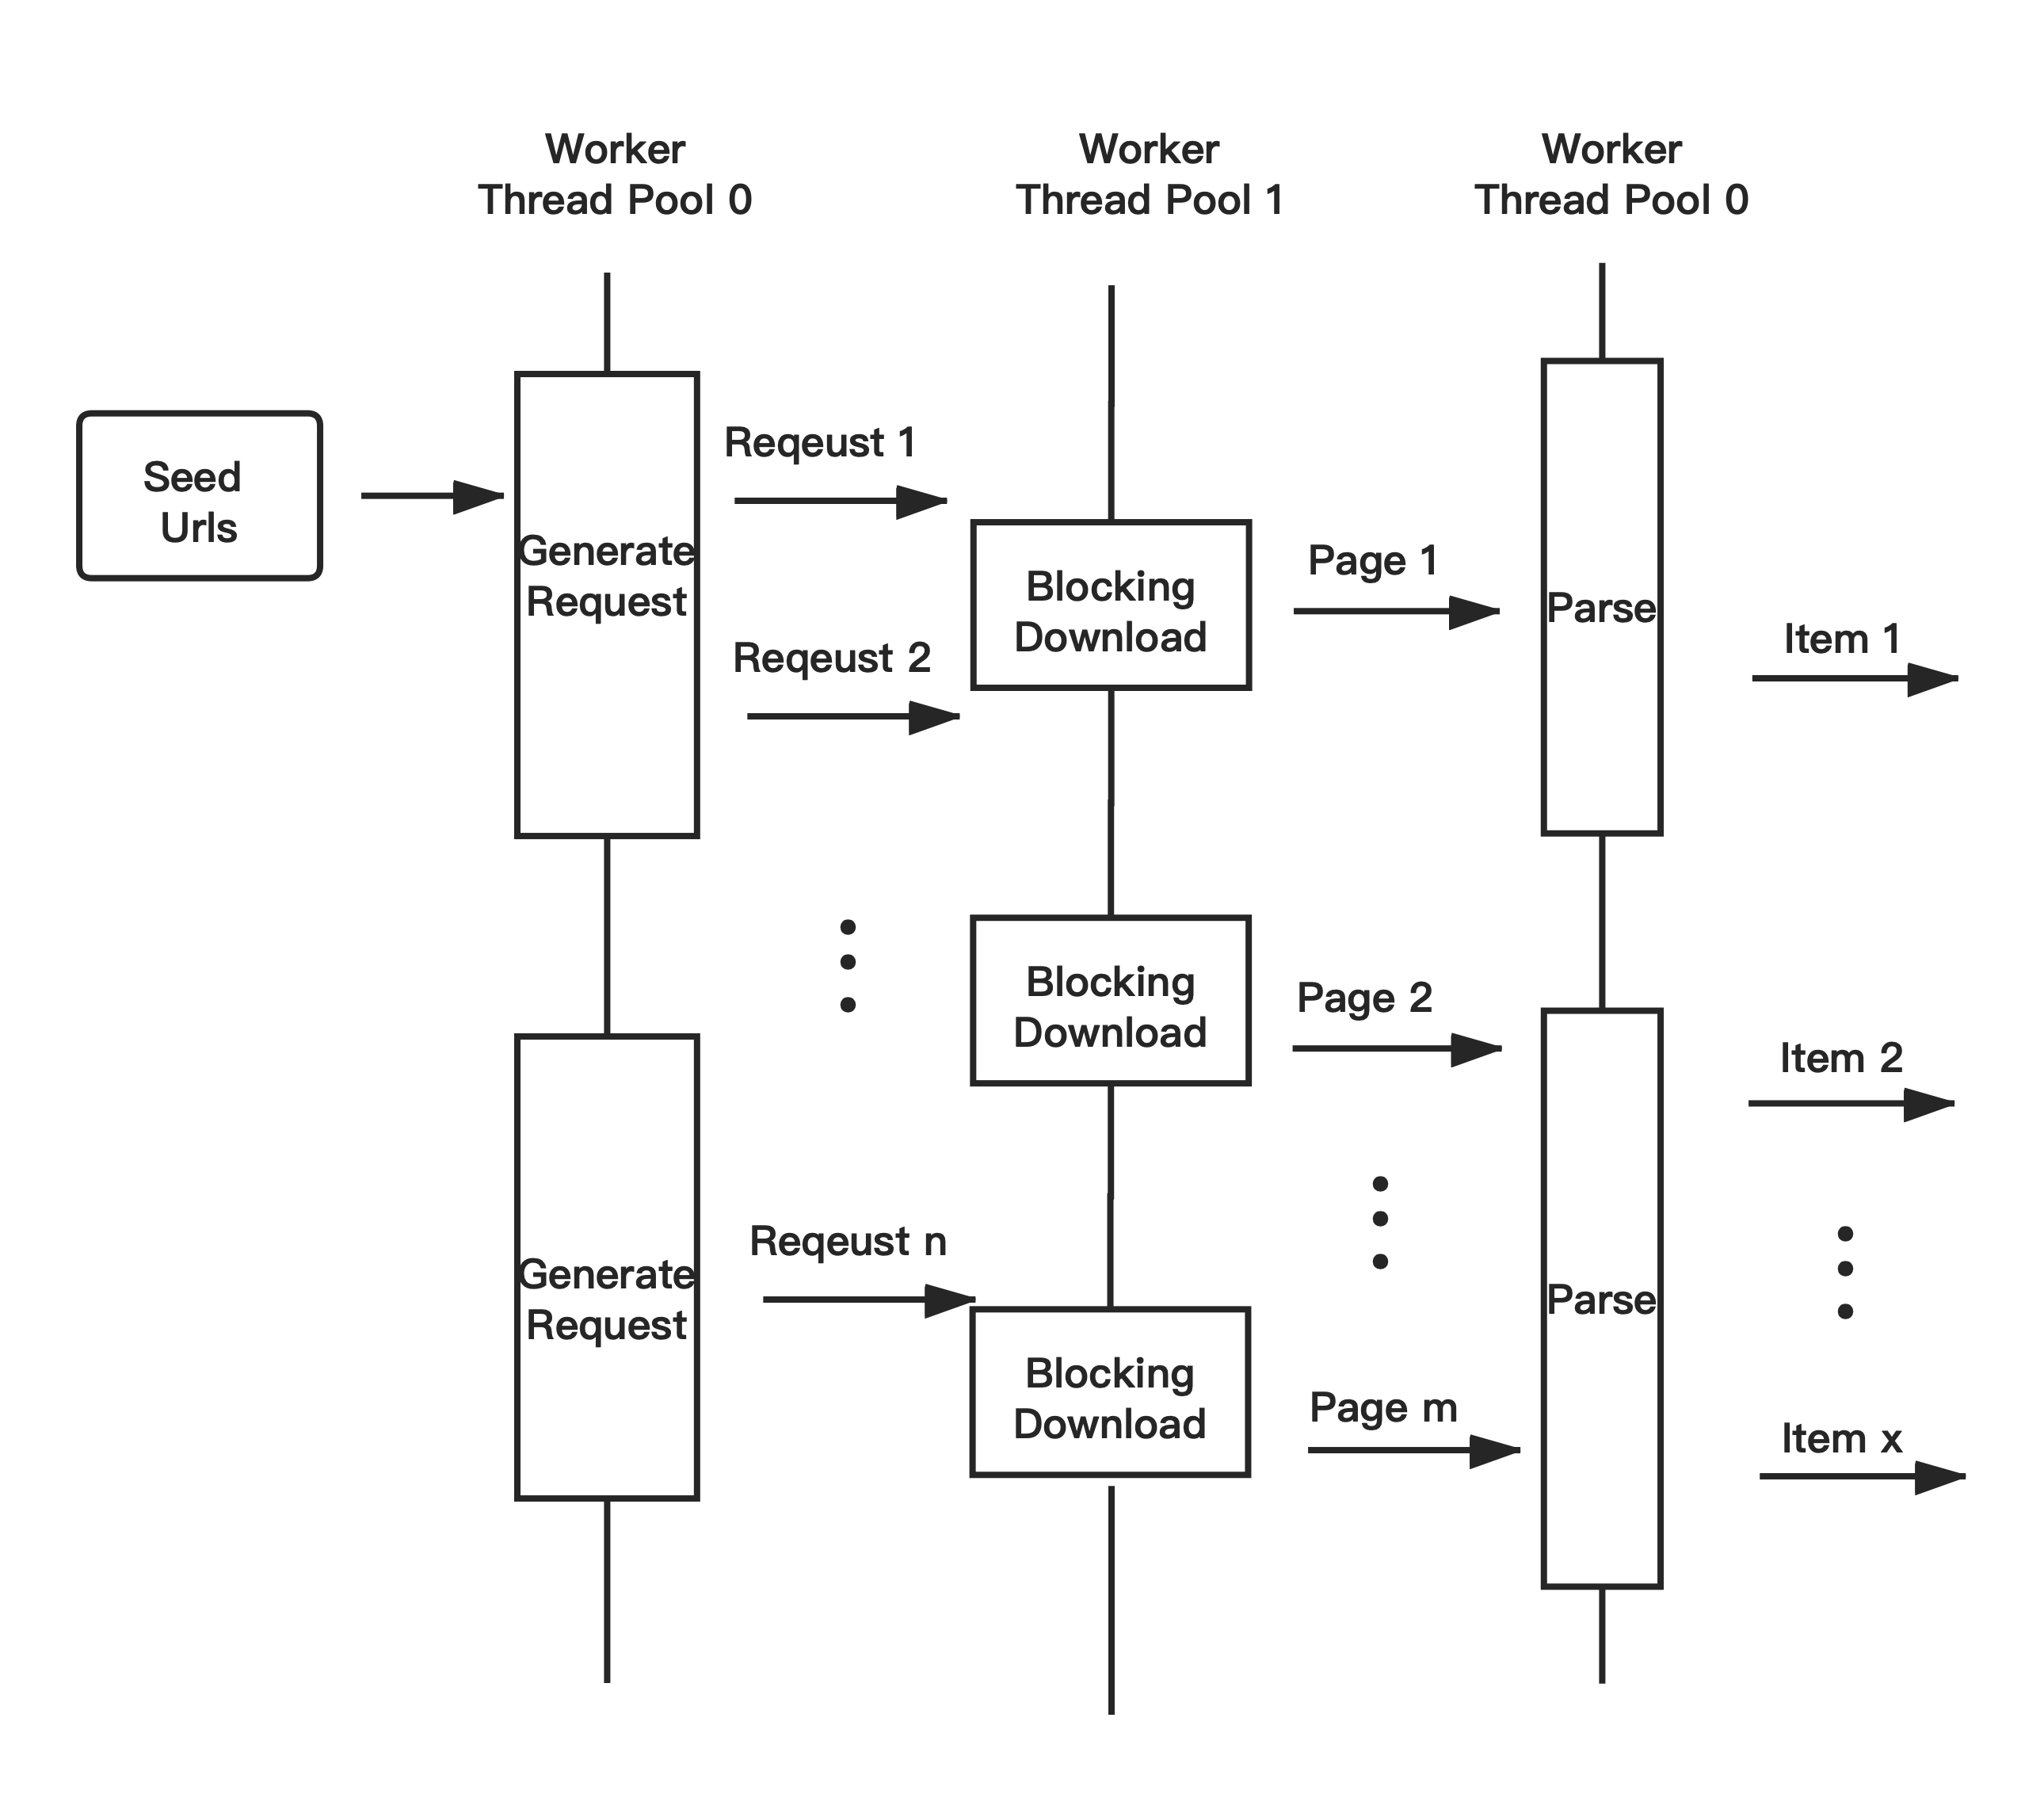
\includegraphics[width= 0.8\textwidth]{pic/reactive-crawler.png}
\caption{响应式爬虫编程模型}\label{fig:crawler}
\end{figure}



% 多种模式对比,我们能发现reactive 爬虫能够最大限度地利用硬件资源。

响应式爬虫编程模型关注于组件算子操作和数据流生成,并对组件算子内部代码的实现提出约束。同时基于该编程模型,本文还提出了
一种基于网站层次树结构的对象模型构造方法,并通过对象模型来配置数据流。

% \subsection{Pull vs Push}

% 提供了Pull模式和Push模式

\subsection{组件非阻塞约束}
异步流式爬虫模型需要保证各个组件的操作都是非阻塞操作,不能阻塞线程,爬虫组件在处理完后,将处理过后的数据通过信号封装
再传播到下游组件中。

爬虫组件中往往都是阻塞代码,阻塞代码会造成线程等待。若通过异步方式运行时,线程则可以执行其他任务,直到阻塞操作完成返回后,再进行相关的处理。
爬虫在下载过程中存在着大量的阻塞网络IO,这个过程如果是采用同步阻塞的方式必然会导致线程的等待,造成资源的浪费。这时,便需要对阻塞代码进行改写或者封装,
将阻塞代码改写成异步非阻塞代码,把阻塞代码调度到隔离的工作线程池中运行,不影响爬取的主流程。爬取流程中的其他阻塞代码也是通过相同的方式转换。

% \begin{figure}[htbp]
% \centering
% 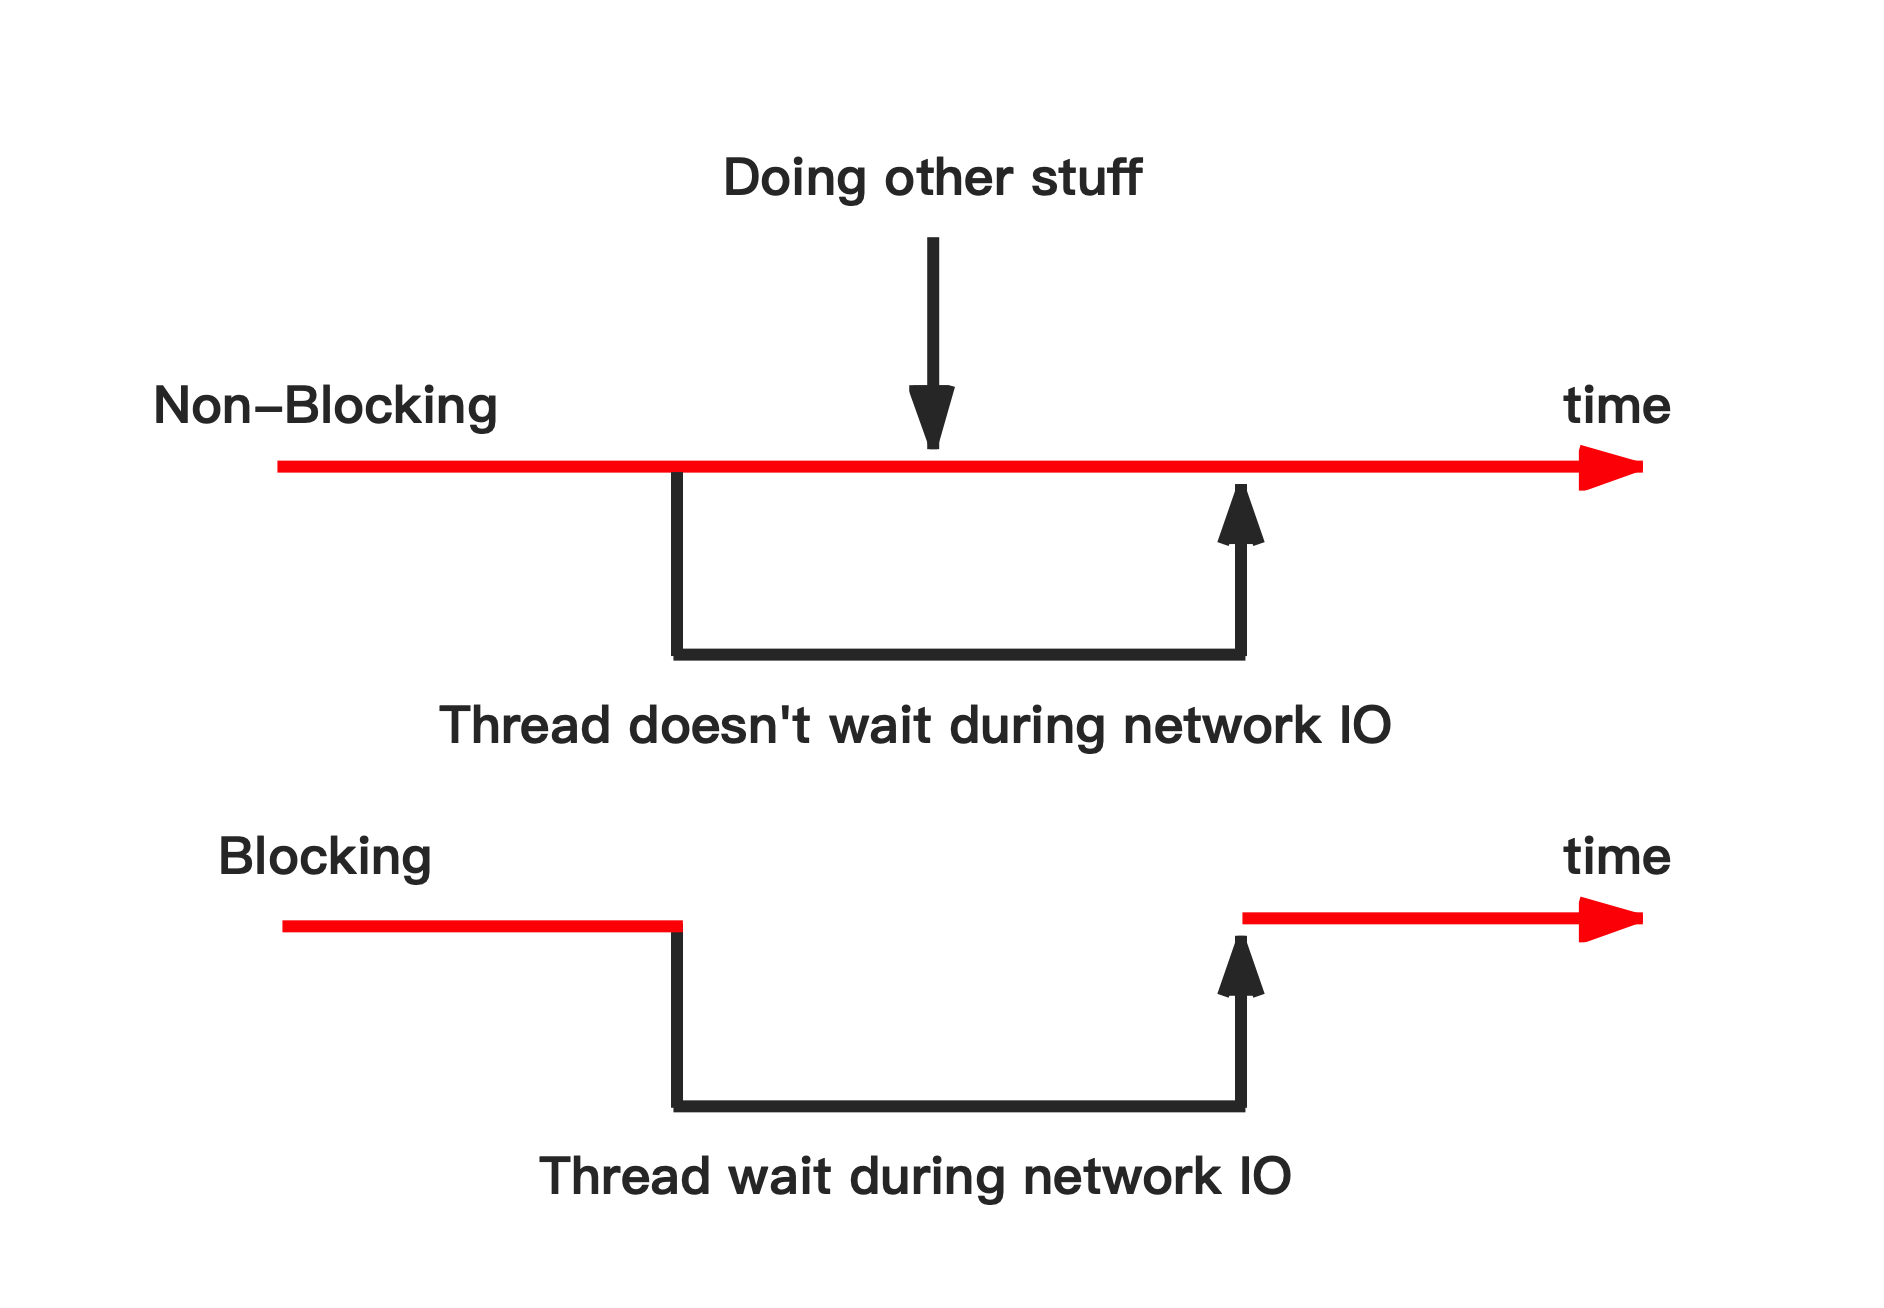
\includegraphics[width= 1\textwidth]{pic/blocking.png}
% \caption{阻塞vs非阻塞}\label{fig:block}
% \end{figure}



% \section{Web页面结构}
% 每个网页都可以表示为树数据结构,如图\ref{fig:html}所示。
% html标签是HTML文档的最基本元素,往往成对出现,并且由开始标签和结束标签构成,如<html></html>,<p></p>, <div></div>等等,
% 这些标签按照一定的规则可以嵌套使用。一个基本的html页面,至少有head头部标签还有body标签。Web页面可以看作是标签树结构。
% 我们往往通过前文提到的Xpath或是CSS选择器来对Web页面结构解析,获取目标属性。
% \begin{figure}
% \centering
% \includegraphics[width=\textwidth]{html.png}
% \caption{Web页面结构 \cite{grigalis2014using}}\label{fig:html}
% \end{figure}

% \section{网站结构分类}

% 网站结构是网站对其表现内容的组织形式\cite{rheinlander2016potential},即网站的各个子页面是如何相互链接的。网站结构又分为物理结构和逻辑结构。
% 物理结构是指网站目录及所包含文件所存储的真实位置所表现出来的结构\cite{singh2014web},物理结构一般包含两种不同的表现形式:扁平式物理结构和树形物理结构\footnote{https://www.searchmetrics.com/glossary/website-structure/}。扁平物理结构是指所有页面都放在根目录下,而树形物理结构则是网页可能存放在二级三级或者更多层级的子目录下,相比之下扁平物理结构简单,容易实现,比较适用于
% 小型网站,树形结构则能更好地维护网页,适用于大型网站\cite{boldi2004ubicrawler}。

% 与物理结构不同,网页的逻辑结构是用来描述网页间的链接关系,而不是页面的存储定位。同样地,逻辑结构也可分为树状结构和扁平结构。
% 通常意义上,爬虫往往是根据网站的逻辑结构也就是网页间的链接关系,进行网站的遍历,后面我们着重描述网站的逻辑结构。

% \subsection{树状逻辑结构}
% 树状逻辑结构往往通过分类或是子栏目进行延伸,其深度往往大于2,通过页面与页面的链接来组织的结构\footnote{https://web.nmsu.edu/~headrick/treestru.html}。网站首页是树形结构的root节点,然后通过链接关系
% 创建边关系,不断地向下分叉,创建新的关系。由于树状逻辑结构比较灵活,且能描述大型网站的页面关系,所以目前大部分网站都是采用的树状逻辑结构\cite{chen2018improving}。

% 事实上,如果只根据链接来创建树的边关系,真正的网站往往是一个网状结构或者是图结构,但我们在构建这样的树形逻辑结构时,往往把已经在树中的节点给忽略,不创建
% 这样的边关系,这样变定义了树状逻辑结构。这和我们的爬虫逻辑也是一致的,不爬取已经爬取过的页面,而是继续地向下寻找未爬取的页面。

% 如图\ref{fig:tree}中,我们发现Home page是根节点,提供有关网站的一些基本信息以及指向外部网站和下属页面的链接,它的下属节点可能会链接到这个网站的其他
% 网页节点或者是其他网站的链接。对于每个下属页面至少4个链接\cite{thalheim2004website}:
% 树形结构中当前页面级别的上一页;
% 树形结构中当前页面级别的下一页;
% 当前页面的父页面;
% 网站主页。


% \begin{figure}[htbp]
% \centering
% \begin{minipage}[t]{0.48\textwidth}
% 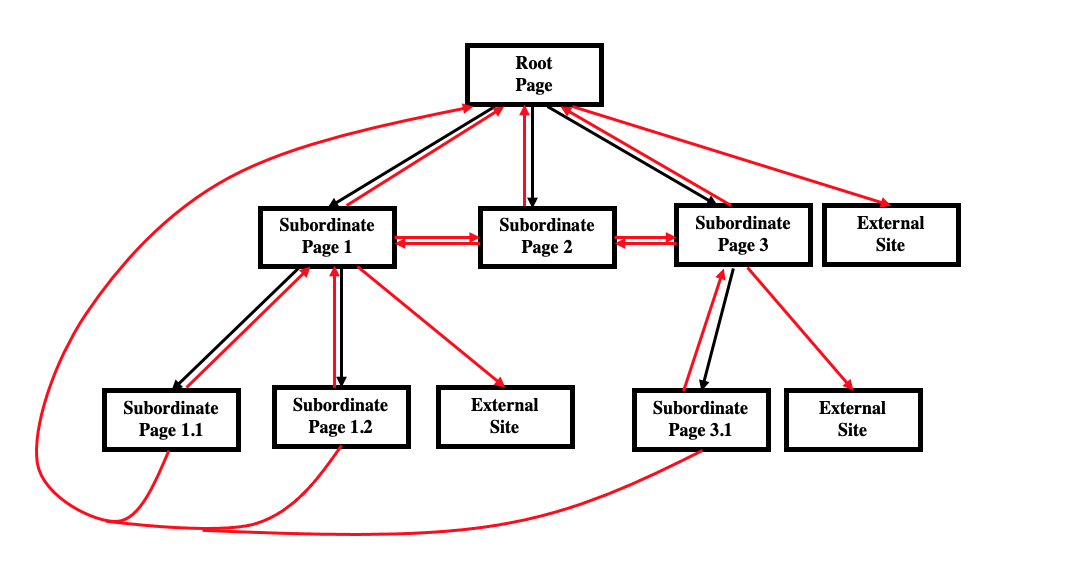
\includegraphics[width=\textwidth]{tree.png}
% \caption{树状逻辑结构}\label{fig:tree}
% \end{minipage}
% \begin{minipage}[t]{0.48\textwidth}
% 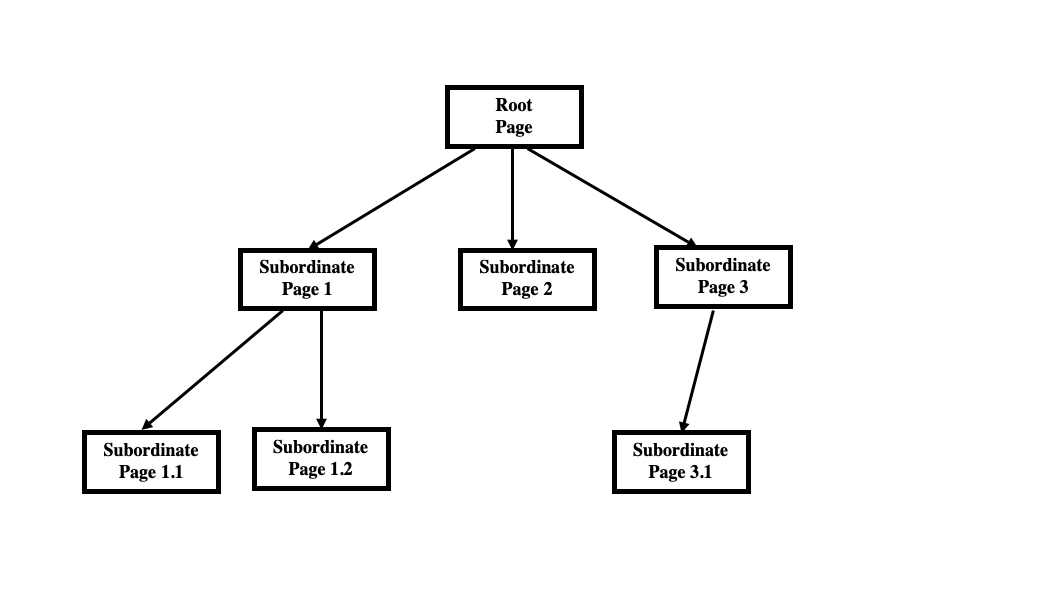
\includegraphics[width=\textwidth]{modified.png}
% \caption{修剪后的树状逻辑结构}\label{fig:modified}
% \end{minipage}
% \end{figure}

% 考虑到树状逻辑结构描述的是网站的内在链接的组织方式,外部网站页面节点可以删除,同时删除边关系。
% 对于内部节点来说,还存在着同层次页面之间的关联关系,通过对边关系的修剪,最后得到图\ref{fig:modified}修剪后的树状逻辑结构。


% \subsection{扁平逻辑结构}

% 扁平逻辑结构也是一种比较常见的网站结构,它往往以网站首页作为“根”,然后从网站首页出发,链接其他页面,一般来说网页链接的深度不会太大。
% 其实如果广义来看,扁平逻辑结构也可以看作是高度为2的树形结构。许多政府网站往往采用的就是扁平逻辑结构。

% 如图\ref{fig:hi}所示,扁平网络结构层次很浅,往往是1层或者两层,从首页Home Page出发,其首页链接到其他的二级页面,二级页面中包含了
% 各式各样的属性。像这样的网络结构其编程模型便比较简单,很容易表示网页结构数据与对象模型之间的映射关系。但目前的大型网站都没有采用扁平式结构了,
% 当然在其局部区域很多大型网站还是存在这样的扁平逻辑结构的。

% \begin{figure}
% \centering
% \includegraphics[width=0.8\textwidth]{hierarchical.png}
% \caption{扁平逻辑结构} \label{fig:hi}
% \end{figure}

% 对于爬虫开发者而言,我们需要定义相应的数据对象模型,该对象模型往往是根据对业务逻辑的理解而创建的,而我们需要做的是将网页数据给映射到
% 我们的对象模型,装填对象来获取目标数据。


% 基于类的面向对象语言,是构建在两个不同实体之上的:类和实例。一个类表示所有对象集合中所具有的特征和属性,我们往往是根据对真实世界的观察和交互,
% 通过编程经验、客观需求以及相关知识来对进行建模,这个建模的过程就是对客观世界的抽象。考虑到爬虫这个具体例子中,我们往往是根据爬虫的经验知识,以及对
% 网页数据结构和网站链接结构的了解,来对爬取的数据模型进行建模。但如果考虑真实的业务场景,把爬虫作为数据源,我们的业务模型定义应该是与爬虫的数据模型无关的。
% 因为业务模型的定义需要关注业务逻辑的实现,而不是数据源的数据类型。所以为了让业务模型与爬虫网页结构模型直接产生联系,我们定义了数据模型映射关系,把网络环境
% 看作存储介质,将网页结构数据与业务模型关联起来。
\subsection{网站结构映射}
% \subsubsection{网站结构}
网站结构是网站对其表现内容的组织形式,即网站的各个子页面是如何相互链接的。真正的网站往往是一个网状结构或者是图结构,网页是图中的一个节点,网页之间通过
超链接作为边。传统爬虫遍历网站的图结构,忽略了网站的层次结构,只关注当前页面节点的结构信息以及后续连接的节点页面,往往容易陷入爬取死循环中,同时对于爬取
目标页面的数据解析还需要遍历网页的结构,过程繁琐且可读性差。

为此,本文通过层次树模型对网站结构进行描述,并在响应式编程模型基础上提出了一种对象模型构建方法,解决了网页数据解析繁琐以及爬虫开发效率低的问题。

\subsubsection{层次树模型}
% 通过对网站扁平逻辑结构以及修剪后的树状逻辑结构介绍,我们发现两者都可以通过一个层次树模型来统一的归纳。
为了方便链接的遍历,本文对网站结构进行建模,将网站看作是层次树结构\cite{kleinberg1999web}。如图\ref{fig:Htree} 所示,根节点为Home Page页面,内部节点则是网站遍历爬取过程中的中间页面,叶子节点则是数据节点,携带着结构化的数据。

\begin{figure}
\centering
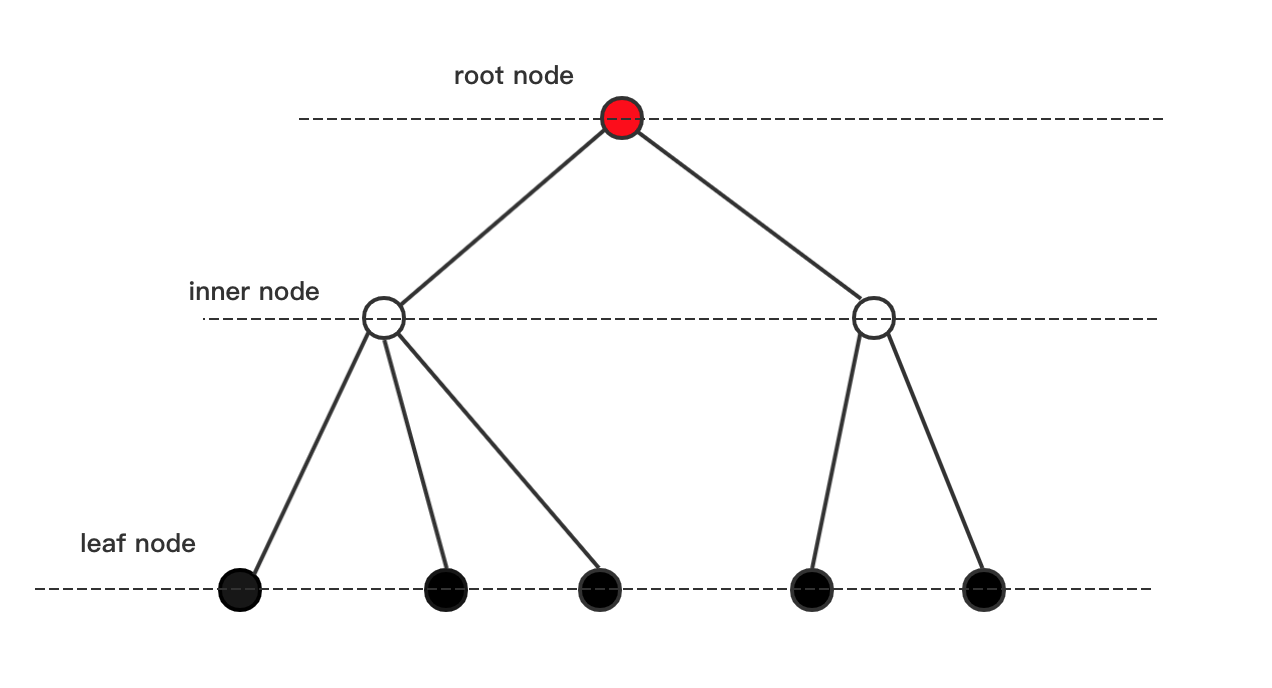
\includegraphics[width=0.8\textwidth]{pic/Htree.png}
\caption{层次树模型} \label{fig:Htree}
\end{figure}


为了描述层次树结构,本文引入了两个类型Node和Link,通过两个元组来表示Node类型和Link类型,即

\[
  Node = [id: Oid, ..., a_i : v_i , ...]
\]
\[
  Link = [from: Oid, to : Oid, ..., b_j : v_j , ...]
\]

在层次树模型中,页面与Node节点一一映射,Node定义中的属性$id$表示唯一标识符,用来区分不同的Node节点,属性$a_i$表示页面中的数据;而页面与页面之间的超链接则表示为Link对象,Link对象描述了Node节点间边的关系,Link对象的$from$属性表示连接的上级页面,$to$属性表示
Link对象连接的下级页面, 属性$b_j$表示链接自身的属性标签。
其中的$Oid$则是URL,网页通过Node节点抽象成了一个数据集合,Node节点的除了id之外的各个属性均表示网页数据,Link用来描述
层次树模型中的边关系,其属性除了表示两端的Node节点外,还包括了链接自身的属性,如链接自身的URL以及链接的描述等等。
当然,并不是所有的页面以及超链接都会在层次树中表示,层次模型其实是对网站的子集的描述。

\subsubsection{对象模型定义}
从三层的层次树模型考虑,第一层是网站首页,也就是root node节点;第二层则是从首页链接出去的内部节点页面,是inner node节点;第三层才是要爬取的目标页面,leaf node节点。
% 很多大型网站局部也是存在的这样的层次结构的,往往第一层是列表页,第二层则是目标页面,而爬虫爬取的目标数据就存放在目标
% 页面上。假如我们把网站首页也看作是列表页,那这样的层次结构就是“列表页{\zhdash}目标页”结构。

如图\ref{fig:mapper} 所示,为了能够描述层次树模型与对象模型之间的映射,我们通过自定义注解来映射数据对象与网页结构间的关系。
如上文所示,层次树模型将网页节点分成了三类,我们需要能够描述这三类节点的层次结构。
其中StartUrls用来描述网站首页,表示数据的爬取起点,也就是层次树结构的root节点;InnerUrl则是表示中间页面,通过中间页面URL的
匹配模式给爬虫提供链接跟进的方向;TargetUrl则是表示目标页面,通过描述目标页面的URL的匹配模式来指定爬取的网页,其描述的是层次
树中的叶子节点,也就是包含结构化数据的节点。这三个注解都是类注解,通过注解的定义,一个
网站的层次树模型也就描述清楚了。然后是属性注解Selector,该注解是为了描述对象属性与网页元素之间的映射关系,
在网页上,数据被包含在HTML元素中,需要通过Selector选择器进行元素定位。
最后通过映射类Entity与叶子Node对象建立映射关系,而层次树中的Link关系则是通过StartUrls、InnerUrl以及TargetUrl之间的层级依赖来
表示。在下一章系统实现部分,本文讲述爬虫是如何根据这种映射关系
进行链接跟进以及页面解析的。

\begin{figure}[htbp]{}
\centering
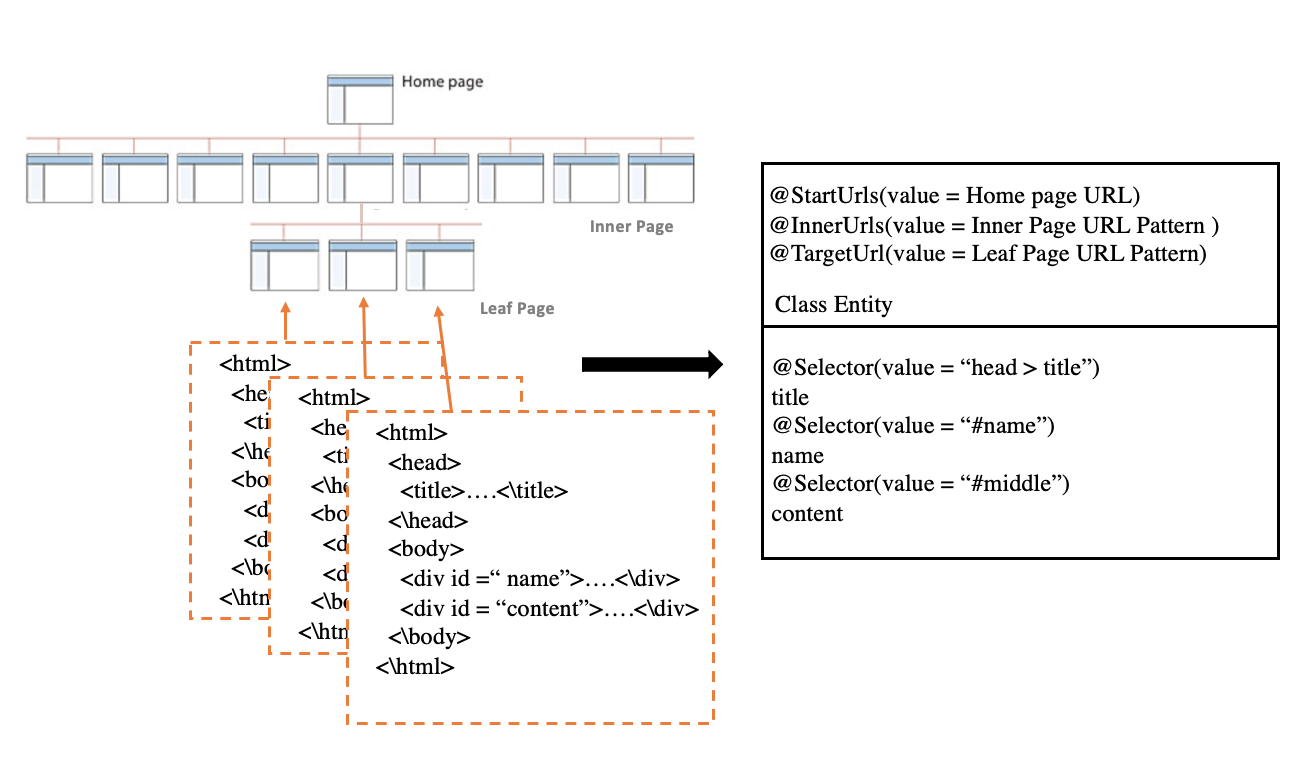
\includegraphics[width= 0.8\textwidth]{pic/mapper.png}
\caption{层次树模型映射}\label{fig:mapper}
\end{figure}

相比于现有爬虫框架,层次树模型能够简化爬虫解析路径的编写,并且通过层次结构避免了爬虫死循环陷阱。开发者无需定义每个层次页面的处理逻辑,同时将爬虫的页面解析和爬虫的页面跟进逻辑
分离开来。爬虫只需要定义对象模型,根据注解建立映射关系,描述网站层次结构,之后传统爬虫框架所需要的页面解析以及后续链接跟进都无需开发者描述,我们会对对象模型
进行解析,自动化生成页面的解析逻辑以及待跟进链接的提取,以此来避免了爬虫繁琐的页面解析规则以及爬取链路的配置,提高爬虫开发的效率。

% 对于层数较高的层次树模型来说,映射方法是一样的,也能很方便地将层次结构模型映射到对象模型中。下一章系统实现部分会介绍如何根据对象
% 模型来初始化Request数据流,并通过一系列组件构建异步数据流。
\subsection{异步数据流构建}
相比于前文提到的三种编程模型,Reactive流式爬虫不需要再维护一个待爬取URL队列,而是通过数据流的形式表示待爬取的URL请求。
为了获取待爬取的Request数据流,爬虫必须明确链接的遍历方式。

如图\ref{fig:model} 所示,爬虫首先会根据上文定义的对象模型来构造一个Request数据流;
之后设置对Request数据流的操作,将Reqeust转化成page,得到中间的Page数据流;
然后对Page设置了解析操作,将解析出来的链接封装成Request,再重新导入到Request数据流中,
同时对页面解析数据解析,将页面映射成数据对象。最后生成一个对象流,以供后续的处理。

整个爬虫过程都被描述成了对数据流的处理,通过数据流之间的算子来描述数据处理过程,
这个过程是异步非阻塞的,因为每个算子计算时是通过信号来触发的。下游的算子接收到上游算子处理后的数
据后,进行相应的处理,再将数据封装成信号传播到下游节点。

通过将各个算子进行组合,构建了异步数据流。数据在整个异步流程中向下传播,不断地处理转换,最终得到结果数据。

\begin{figure}[htbp]
\centering
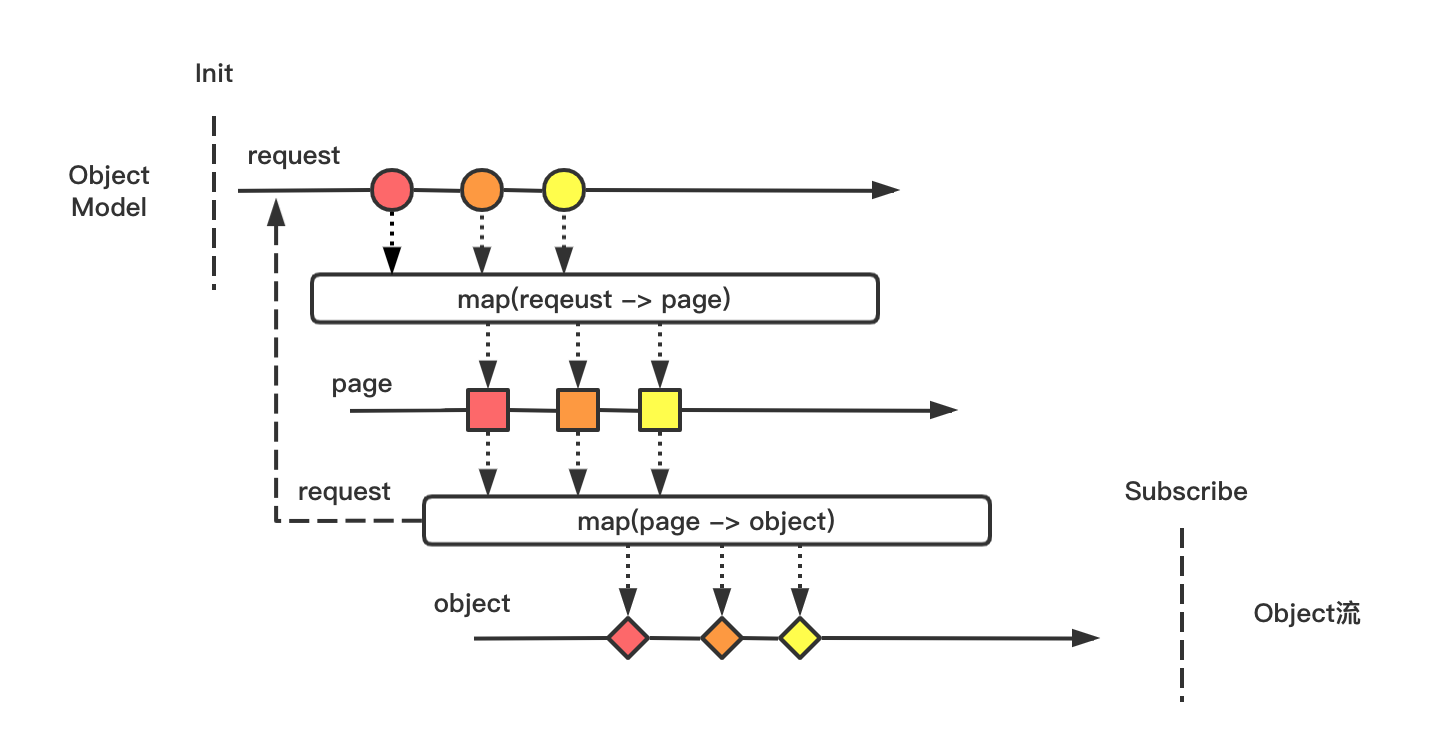
\includegraphics[width= 1\textwidth]{pic/reactive-model.png}
\caption{异步数据流}\label{fig:model}
\end{figure}

\subsubsection{异步数据流构建算法}
爬虫本身就是对网站的遍历,爬虫通过遍历整个层次树结构来构建异步数据流。本文通过基于剪枝的广度优先搜索的方法对树结构进行遍历,获取需要爬取的链接,
将链接导入到Request数据流中。数据爬取遍历过程如算法\ref{algorithm} 所示,用户从对象模型出发,会对对象模型解析,生成Request数据流。
当数据流中有数据时,会通知下游进行处理。将通过数据流中的URL去请求网页,对网页进行异步下载,之后将网页进行解析,得到当前网页的所有链接。这里采用的是
广度优先搜索方法对链接进行跟进,同时为了防止搜索空间过大,本文通过链接正则匹配的模式来跟进链接,缩小搜索空间。


\begin{algorithm}[htbp]
 \caption{异步数据流构建算法}
 \label{algorithm}
 \begin{algorithmic}[1]
  \REQUIRE $m$代表定义的对象模型,$stream$表示Request数据流, $targetUrl$表示目标页面匹配模式, $pattern$代表目标链接匹配模式, 
  \STATE $visited$ $\gets$ \{\}
  \STATE $s$ $\gets$ parse($m$) 解析对象模型获得初始爬取起点
  \STATE EmitNext($stream$, $s$) 初始化数据流
  \STATE $result$  $\gets$ \{\}
  \WHILE{ $stream$ $\neq$ $\varnothing$}
    \STATE $url$ = OnNext($Stream$) 数据流中的数据到达
    \STATE $visited$.Append($url$)
    \STATE $page$ = AsyncDownload($url$) 页面下载
    \STATE $links$ = AsyncLinkExtract($page$) 页面解析
    \IF {$url$ $\textbf{Match}$ $targetUrl$}
      \STATE $r$ = Parse($page$)
      \STATE $result$.Append($r$)
    \ENDIF
    \FOR{$link$ $\in$ $links$} 
      \IF{ $link$ $\notin$ $visited$ and $link$ $\textbf{Match}$ $pattern$}
        \STATE EmitNext($stream$, $link$)
        \STATE $visited$.Append($link$)
      \ENDIF
    \ENDFOR
  \ENDWHILE
 \end{algorithmic}
\end{algorithm}



% \section{异步流式爬虫模型}

% \subsection{数据流操作}
% 外部配置通过数据流组合的形式进行处理。爬虫编写过程中,往往需要考虑爬虫的配置情况。针对于不同的场景,配置的要求也不同。
% 我们需要将静态的数据转化成动态数据流,通过和Request数据流组合,使得每一个Request都有自己对应的User Agent、Cookies以及
% 代理IP。
% 爬虫行为被描述成了对数据流的操作,爬虫的代理IP、Cookies、User Agent配置则是描述成了数据流的组合。同时爬虫爬取频率设置则可以被描述成对Request数据流各个元素的延迟操作,如图所示,
% 每个Request请求被delayElements操作延迟固定的时间间隔到达下游节点,我们考验通过设置延迟的大小来调整爬取的频率。
% 另外,爬虫爬取数量可以通过take算子控制,该算子将下游的数据请求方向传播到上游节点,控制Request数据流往下游传播的Request数量。一旦达到了
% 设定的值,就结束整个Request数据流,爬取流程也随之停止。
% 爬虫的异常处理则可以通过对数据流error信号的监听,捕获每个算子操作时异常进行处理。

% 总的来说,通过异步流式爬虫模型,我们能够在上面进行很简单的操作来对爬取过程进行配置。

% \subsection{组件封装}
% 爬虫的各个组件也可以描述成对数据流的Map,Filter以及FlatMap等操作,基于Reactor提供的各个算子,我们可以对各个组件进行封装。
\subsection{反反爬策略设置}\label{section-anti}
大多数网站都设置相关的反爬策略,本文仅从研究的角度来实现响应式爬虫模型的反反爬策略的配置。
由于响应式爬虫模型是对数据流的异步操作,爬虫在设置反反爬策略时,是通过对数据流的处理来实现。
响应式爬虫模型是基于响应式编程来实现的流式爬虫,提供了许多算子来对数据流进行处理,我们可以
通过这些算子来对爬虫的Request数据流、Page数据流以及最终被消费的对象数据流进行处理。

对于网站IP限制的问题,爬虫通过调整IP爬取的频率和次数来应对。响应式爬虫通过对数据流中数据加上延迟
的限定来处理。如图\ref{fig:delay} 所示,通过delayElements算子,将每个Request请求都设定相应的时间间隔,这样
减少请求的频次,减缓了被爬取网站的负载。


\begin{figure}[htbp]
\centering
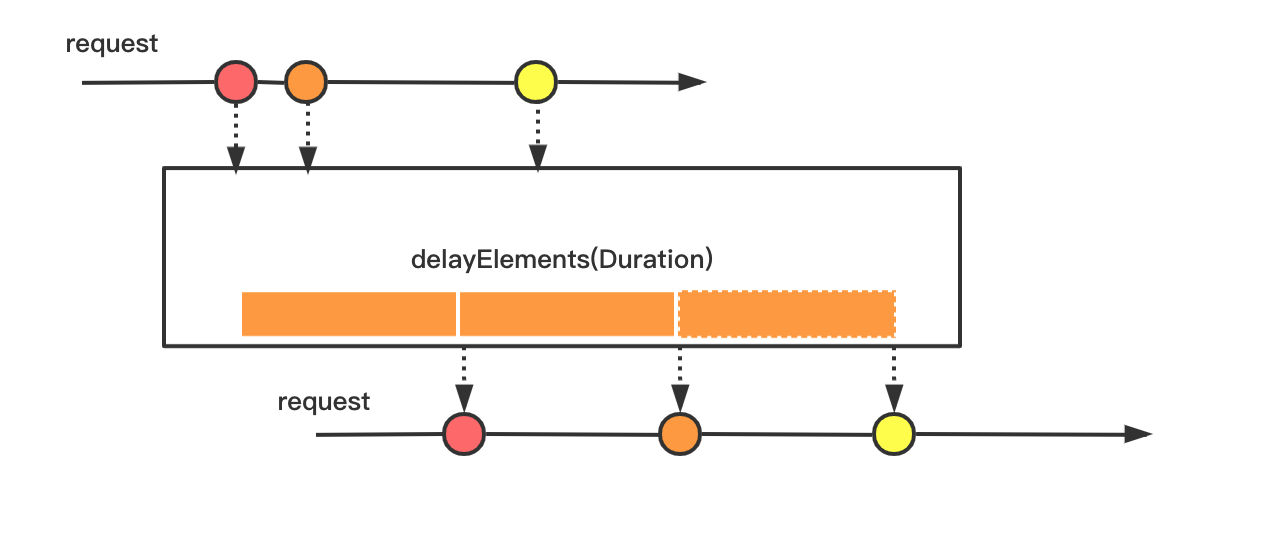
\includegraphics[width= 1\textwidth]{pic/delay.png}
\caption{爬虫频率配置}\label{fig:delay}
\end{figure}

针对于网站的UA限定、IP限制,Cookies限制以及验证码等问题,响应式爬虫模型通过构建User Agent数据流、代理IP数据流和Cookies数据流来对Request数据流进行操作。
如图\ref{fig:zip} 所示:通过与各个配置流的组合,每个Reqeust配置相应的User Agent,都有各自的代理IP以及Cookies设置。
另外在User Agent流、代理IP流以及Cookies流生成时,同样可以配置相应的策略,例如设置User Agent、IP以及Cookies的更换频次等。

\begin{figure}[htbp]
\centering
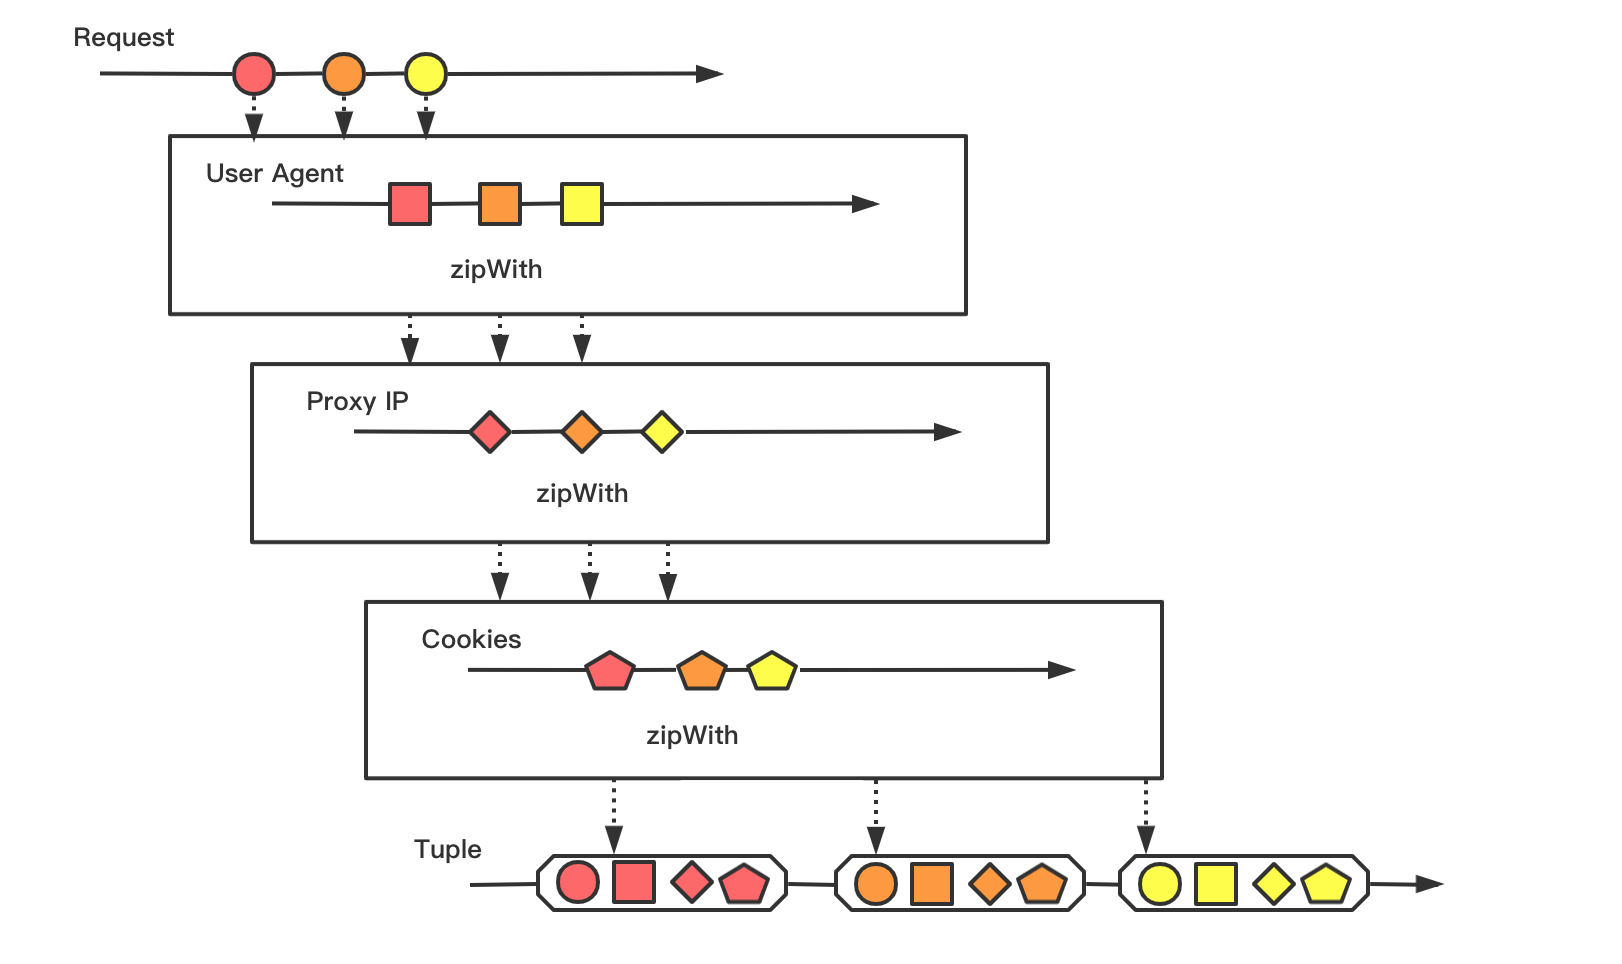
\includegraphics[width= 1\textwidth]{pic/reactive-zip.png}
\caption{Request数据流配置}\label{fig:zip}
\end{figure}


对于反爬策略中次数的限定可以通过take算子来解决,同时take算子提供了相应的背压机制,通过limitrate来对上游的组件进行流量控制。
如图 \ref{fig:take}所示,能够根据爬取数量来设置爬虫的停止的条件,当爬取到一定数量的数据后,下游组件会将cancel信号传播到上游组件,最后
停止爬虫的爬取,而limitrate则向上游反馈下游组件的消费能力,防止生产者生产速度远远大于消费者消费速度,引起任务的大量堆积。

\begin{figure}[htbp]
\centering
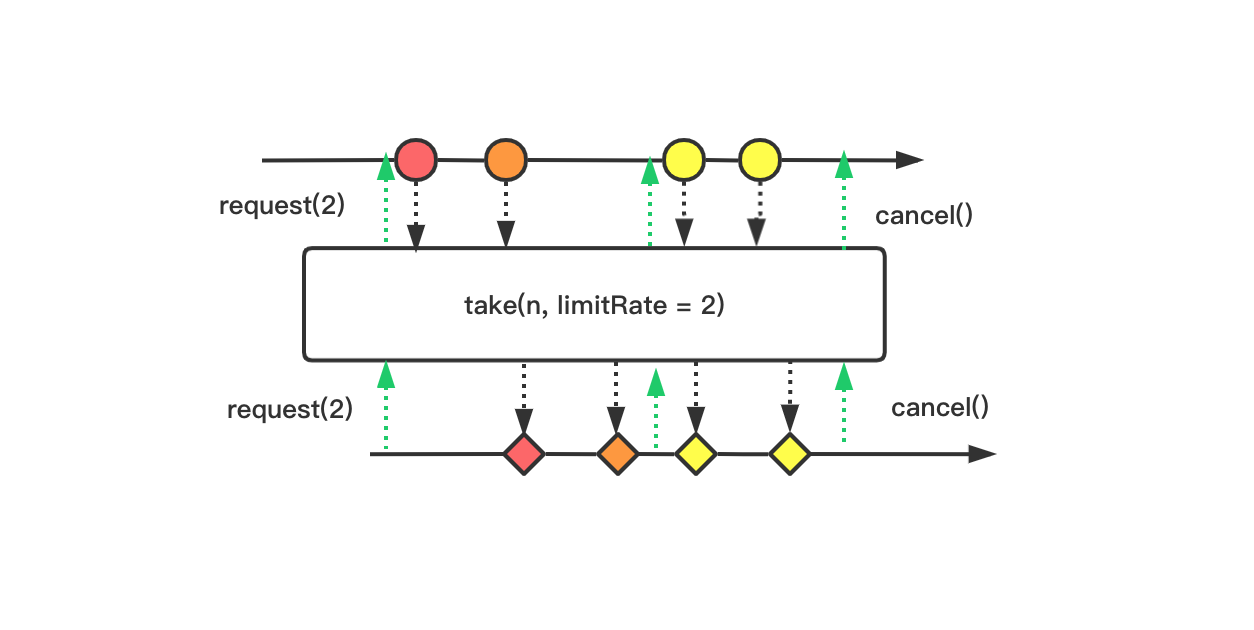
\includegraphics[width= 1\textwidth]{pic/reactive-take.png}
\caption{爬取次数限制和背压配置}\label{fig:take}
\end{figure}


\section{本章小结}
本章从网站结构出发,概述了三种爬虫编程模型,并分析各个模型的优劣,提出了一种响应式爬虫编程模型,
从对数据流处理的角度,介绍了爬虫爬取模型的运用场景。

下一章介绍响应式爬虫模型的具体实现。


%%%%%%%%%%%%%%%%%%%%%%%%%%%%%%%%%%%%%%%%
%%%%%%%%%%%%%%%%%%%%%%%%%%%%%%%%%%%%%%%%

\chapter{框架实现}\label{Chapter_impletation}
本章介绍响应式爬虫的具体实现,首先介绍了各个组件的基本实现接口以及各个爬虫组件的实现。然后介绍了
系统各个模块的实现以及响应式爬虫开发过程。

\section{Project Reactor介绍}
本文以目前主流的响应式编程库为基础,提出了Spidereact响应式爬虫技术框架。
Project Reactor是第四代响应式编程库\cite{project_reactor},建立在Reactive Streams规范基础上,实现了Reactive Programming编程范式。它能让你
快速地构建一个遵循响应式编程范式的响应式系统,提供完全无阻塞的异步数据流操作。

Project Reactor提供了两个基本的数据类型:Mono和Flux。Mono表示0个或1个数据项(数据项有可能是error信号),
而Flux则表示0个或多个数据项,或是一个error。Mono和Flux就是数据源,它们都实现了Pubulisher接口,可以通过订阅这些
数据源并声明操作流程,对这些将要到达的数据进行处理\cite{chen2018improving}。
Spring也对Reactor进行了集成,同时Project Reactor还有很多的扩展,提供了R2DBC,一种响应式关系型数据库连接,将关系性数据库JDBC中的阻塞调用转变成了异步非阻塞模式,
通过整合Spring,Reactor,R2DBC等等Reactive组件,我们就能够构建一个响应式系统。

本文将通过Project Reactor与爬虫框架进行整合,提出一种响应式的爬虫编程模型,来提高在有大量的网络IO场景下爬虫系统的资源利用率。
本文将原有的爬虫框架中的各个组件均通过异步非阻塞的形式组合,构建了一种新的响应式爬虫流程。

\section{爬虫框架模块}
  Spidereact是基于Project Reactor的Java响应式爬虫框架,通过异步数据流,解决传统爬虫框架的一个请求对应一个线程处理的模式存在的问题。
通过Spidereact开发一个爬虫,首先要分析网页数据结构,构建数据对象模型与网页数据之间的映射关系,同时通过Annotation来表明待爬取的URL;对
爬虫的数据初始化组件、页面下载组件以及网页数据解析组件等模块进行组件化声明, 通过对组件的组合构造爬虫处理流程图,执行爬虫获得响应式数据流;
后续可以对得到的数据流进行过滤、筛选和数据持久化操作。如图\ref{pic:all} 所示,Spidereact的各个模块功能介绍如下:
  \begin{itemize}
    \item 数据模型定义模块: 通过自定义注解来定义数据对象与待爬取网页对象直接的映射关系,通过这种映射关系模型来对网页结构中的元素进行解析,同时生成相应的数据对象。
    \item 组件编排模块: 对爬虫的各个组件进行编排组装,最后构建一个爬虫组件流。
    \item 异常处理模块:定义爬虫阶段的各个异常情况,提供相应的异常处理接口,方便二次扩展。
    \item 监控模块: 监控爬虫的各个阶段情况,统计爬取成功次数、失败次数等等。
    \item Web模块:整合Spring,使得Spidereact能够集成到Spring框架中。
  \end{itemize}

\begin{figure}
\centering
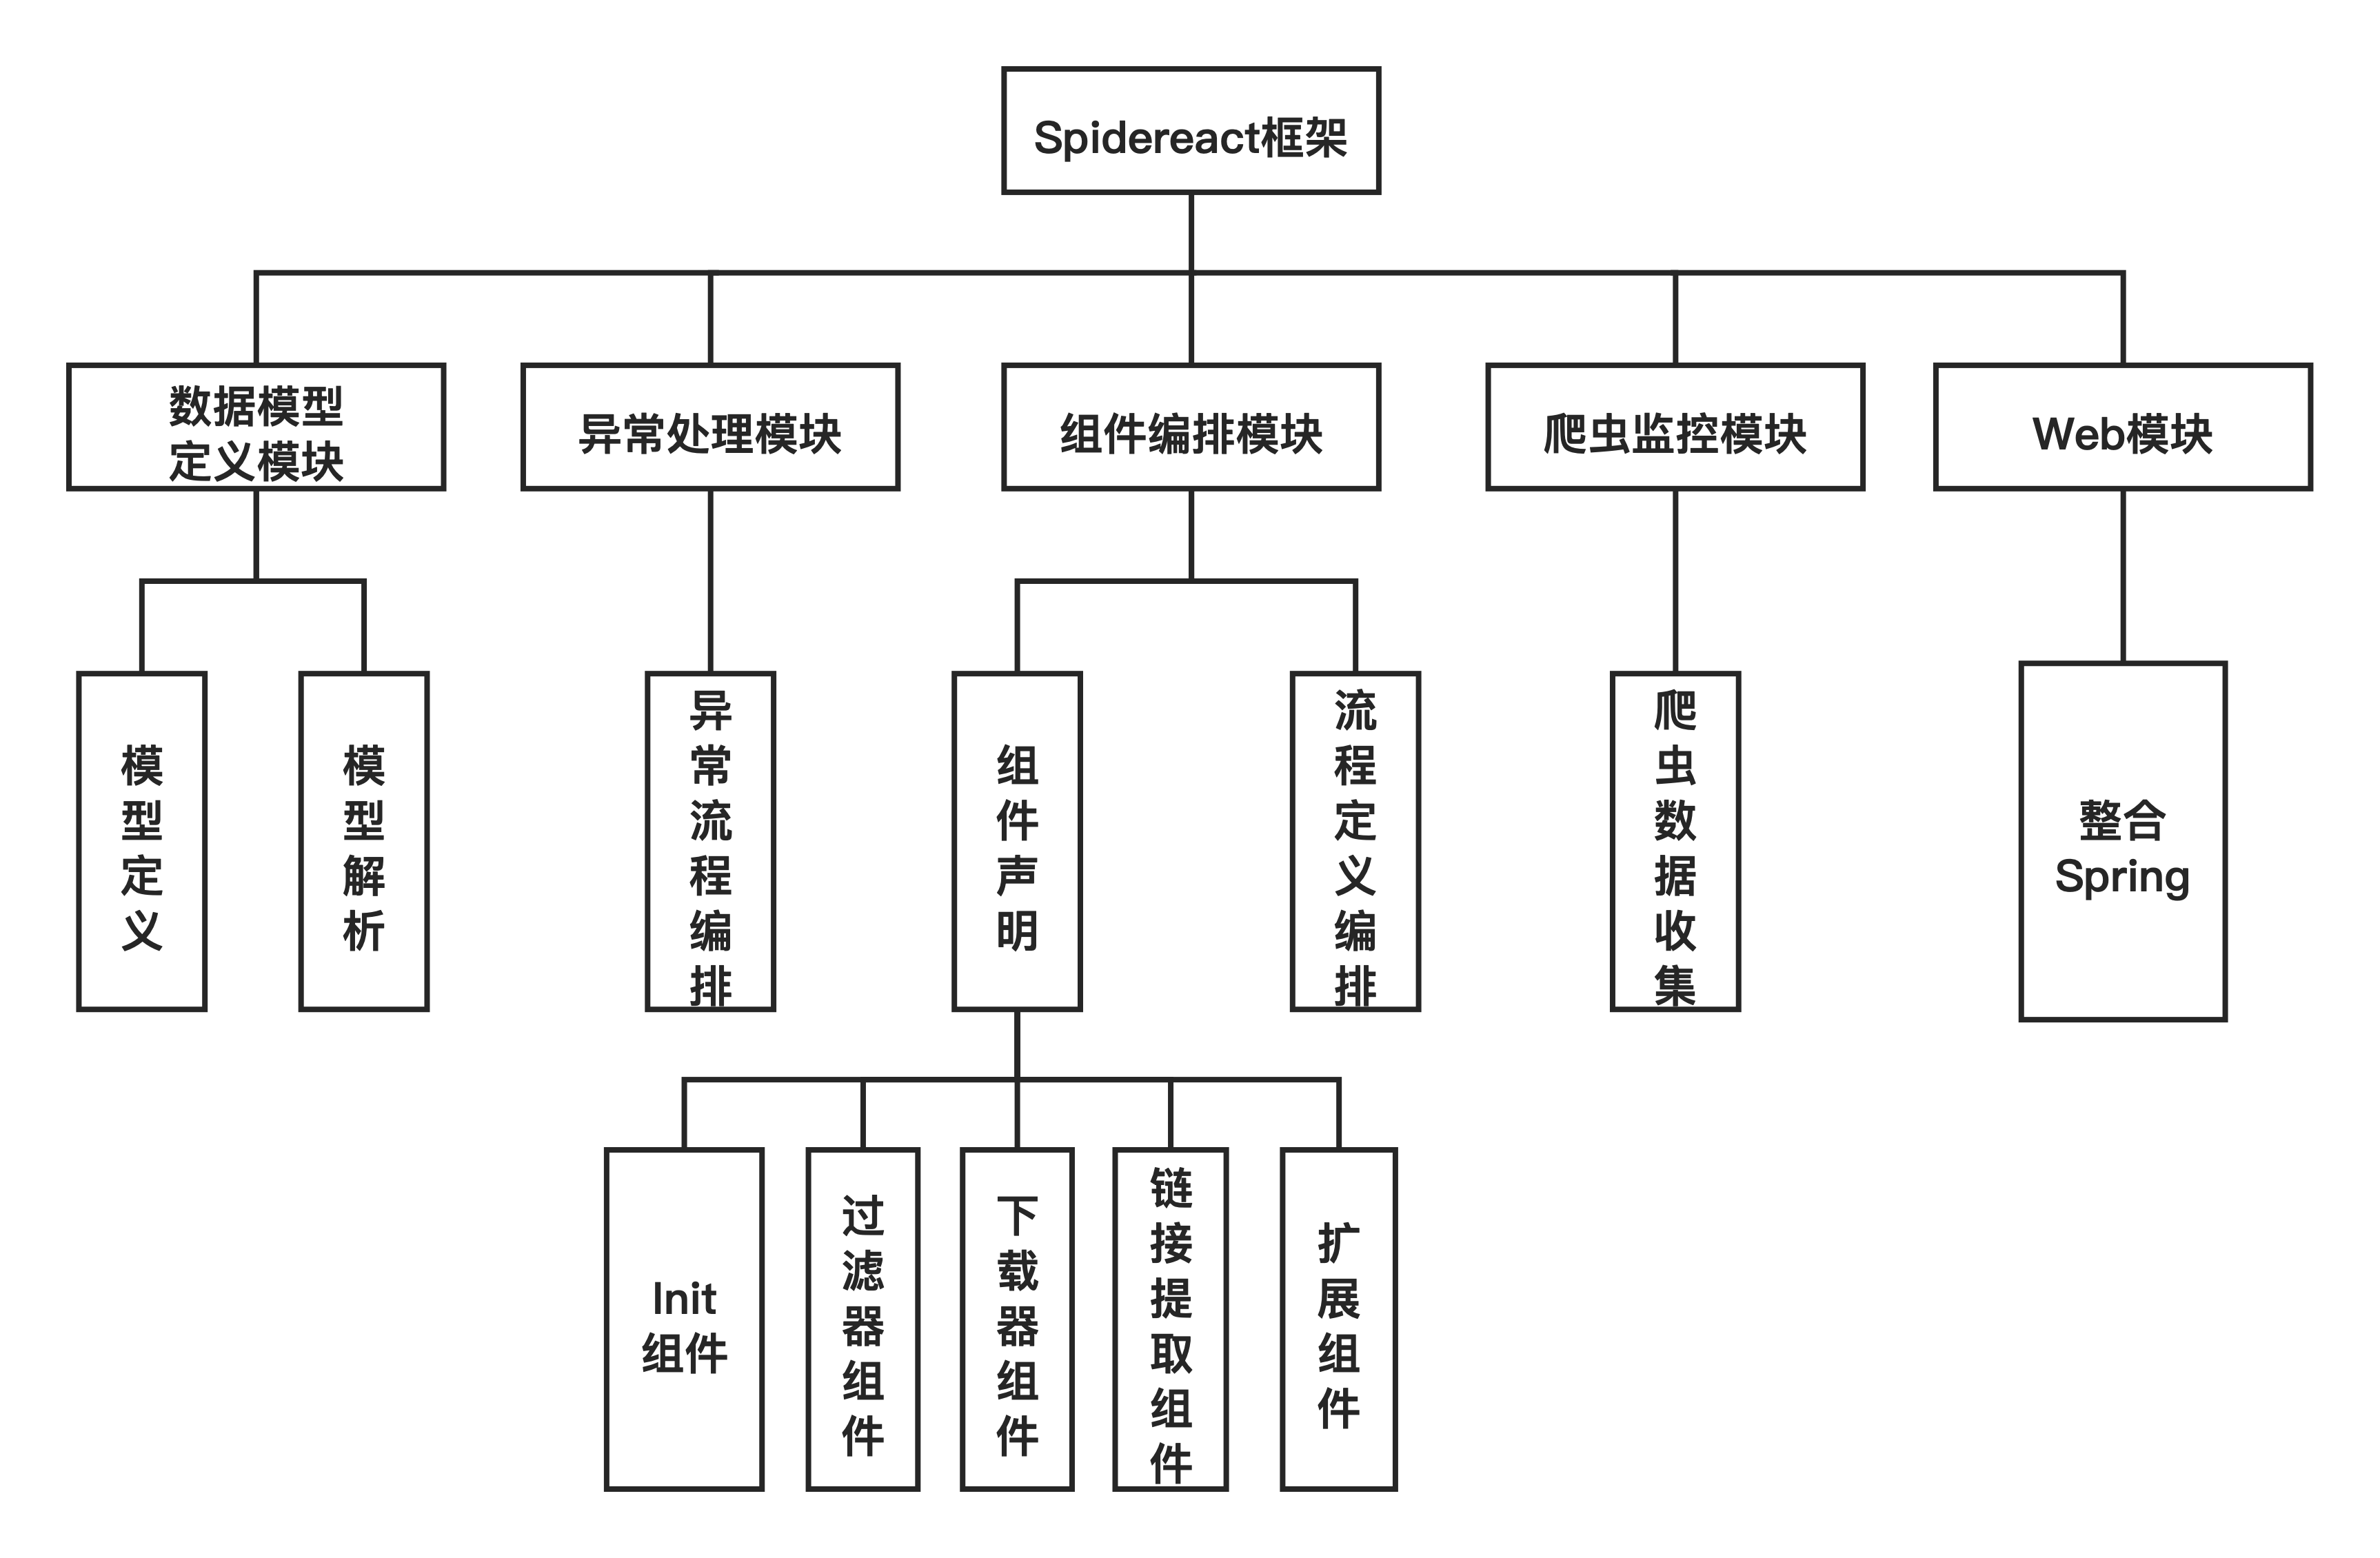
\includegraphics[width=\textwidth]{pic/all.png}
\caption{Spidereact功能模块图}\label{pic:all}
\end{figure}


\subsection{数据模型定义模块}
数据模型定义模块会根据需要爬取的网页的网页结构来定义对应的数据对象,
会通过几个注解来定义爬虫的爬取方向以及定义待解析的数据。如表\ref{table:annotation} 所示,
Spidereact通过StartUrls、InnerUrl、TargetUrl以及Selector来定义数据对象,首先根据StartUrls来构建初始Reqeust数据流, Request数据流用来描述对URL的请求信息。TargetUrl则描述在页面解析过程中需要提取的网页链接,作为后续爬取的URL,
重新导入到Request数据流中。前文也提到了,Selector注解是用来解析网页数据,网页上的数据都是以文本形式读取,而
数据对象中往往有各种各样的类型,这是需要类型间的映射。网页上除了文本以外的图像、音频以及视频数据,需要开发者自定义下载器中
的下载逻辑进行处理。目前支持以下几种类型:

  \begin{enumerate}
    \item String和几种基本数据类型:float,double,int,long,boolean。
    \item java.util.Date类型以及org.joda.time.DateTime。
    \item 属性都由Selector注解的POJO类。
    \item List类型,其中List存储的类型必须是Selector支持的类型。
  \end{enumerate}


定义的数据模型会在爬虫构建的时候进行解析,其中StartUrls中的value属性会被传入Init组件生成初始数据流;
而InnerUrl中定义的中间页面URL模版则会被导入到链接提取组件中,来对网页上的链接进行过滤,然后提取出爬虫
想要爬取的链接,再倒入到数据流中;TargetUrl中定义的目标URL模版用来识别目标页面,然后通过映射组件将网页
映射成数据对象。


\begin{table}
\centering
\begin{tabular}{|c|c|}
\hline
注解 & 描述 \\
\hline
StartUrls & 初始URL列表 \\
InnerUrl & 中间页面URL,用来表明链接跟进的方向 \\
TargetUrl & 目标URL,表明最终要解析的页面\\
Selector & CSS选择器,匹配网页中的元素\\
\hline
\end{tabular}
\caption{主要使用的注解}\label{table:annotation}
\end{table}

\subsection{组件编排模块}
组件编排模块负责对各个爬虫组件的流式构建,开发者只需要关注各个组件具体的实现逻辑,组件处理链路编排则由
组件编排模块来实现,开发者能很方便地构造一个从爬取到解析到数据处理分析的逻辑链路。

组件编排模块的设计参考了工厂设计模式,本文结合图\ref{fig:uml} 来进一步介绍。OperatorFactory负责管理和创建OperatorFlow,它会根据
传入的Flow名字来加载爬虫流程实例,OperatorFlow用来表示爬取流程,管理爬取过程中的各个组件,各流程中组件均可相互复用。
组件编排模块主要分为了两个部分,一部分是基本组件声明,还有一部分则是流程编排。

\begin{figure}
\centering
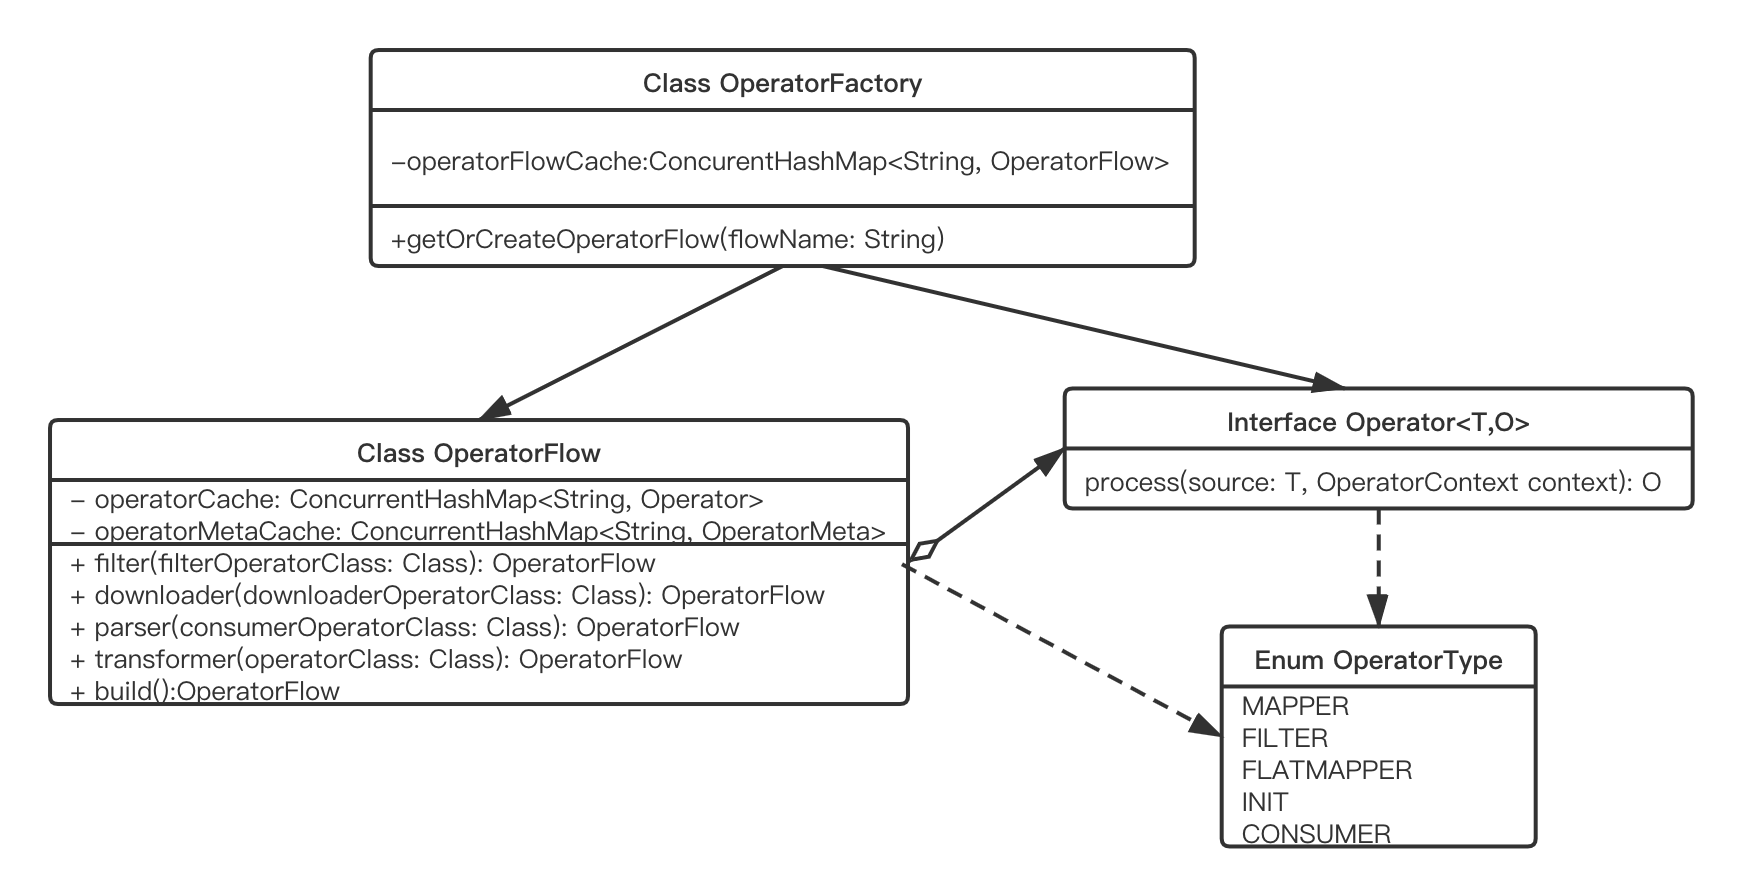
\includegraphics[width=0.98\textwidth]{pic/operatorflow.png}
\caption{组件编排模块UML类图}\label{fig:uml}
\end{figure}

\subsubsection{爬虫基本组件}
在Spidereact的设计中,组件是位于流程之中,具有一定的先后依赖顺序,其中基本组件如初始化组件、下载器组件以及解析器组件的顺序
是固定的。各个组件无法独立执行,必须构建完整的爬取流程才能执行,组件可被复用于不同流程之中。

Spidereact爬虫框架是基于Project Reactor构建的,每个爬虫组件都会被Spidereact给隐式加载成异步非阻塞模式,开发者只需要注重
各个组件的内部逻辑,无需感知流程编排的内部细节。开发者通过声明组件对应的类,而不需要实例化组件,Spidereact会根据声明的组件类在编排
阶段对组件进行实例化,然后编排流程图。

Spidereact会维护一个内部的数据流,各个组件分别对流数据上的数据进行处理,数据在不同组件上传递、处理、转换。
在Spidereact中,数据一定会经历这样一个转变过程,从Request到Page再到Object。如表\ref{table:object} 所示,Request是对一个爬取请求的封装,
包括了请求的URL,请求的请求头,Cookies等等相关信息,Page对象则是对于下载页面的封装。

\begin{table}
\centering
\begin{tabular}{|c|c|}
\hline
类型 & 描述 \\
\hline
Request &  请求的封装\\
Page & 对下载的页面的封装\\
\hline
\end{tabular}
\caption{两种基本数据类型}\label{table:object}
\end{table}

爬虫首先通过Init组件来初始化构造的Request数据流;初始的Request流会经过过滤组件,通过过滤
规则来去除某些不需要再爬取的网页;然后经过
下载器组件的处理,将Request给转换成了Page页面,然后传入下一级组件;链接提取组件在Page数据流上进行操作,提取出Page页面上
所需要的链接,链接再重新倒入到Request数据流中,该组件操作不会对Page数据流中的数据
产生任何影响,然后将Page数据流传到对象映射组件中;对象映射组件会对传过来的Page数据
流进行映射,将Page中的HTML与已经定义好的对象模型进行映射,构建出对象流;同时,Spidereact支持自定义
扩展组件,实现相关的处理逻辑,对对象流进行处理,如数据的持久化存储,数据的展示等等。


\definecolor{dkgreen}{rgb}{0,0.6,0}
\definecolor{gray}{rgb}{0.5,0.5,0.5}
\definecolor{mauve}{rgb}{0.58,0,0.82}

\lstset{ %
  language=Octave,                % the language of the code
  basicstyle=\footnotesize,           % the size of the fonts that are used for the code
  numbers=left,                   % where to put the line-numbers
  numberstyle=\tiny\color{gray},  % the style that is used for the line-numbers
  stepnumber=2,                   % the step between two line-numbers. If it's 1, each line 
                                  % will be numbered
  numbersep=5pt,                  % how far the line-numbers are from the code
  backgroundcolor=\color{white},      % choose the background color. You must add \usepackage{color}
  showspaces=false,               % show spaces adding particular underscores
  showstringspaces=false,         % underline spaces within strings
  showtabs=false,                 % show tabs within strings adding particular underscores
  frame=single,                   % adds a frame around the code
  rulecolor=\color{black},        % if not set, the frame-color may be changed on line-breaks within not-black text (e.g. commens (green here))
  tabsize=2,                      % sets default tabsize to 2 spaces
  captionpos=b,                   % sets the caption-position to bottom
  breaklines=true,                % sets automatic line breaking
  breakatwhitespace=false,        % sets if automatic breaks should only happen at whitespace
  title=\lstname,                   % show the filename of files included with \lstinputlisting;
                                  % also try caption instead of title
  keywordstyle=\color{blue},          % keyword style
  commentstyle=\color{dkgreen},       % comment style
  stringstyle=\color{mauve},         % string literal style
  escapeinside={\%*}{*)},            % if you want to add LaTeX within your code
  morekeywords={*,...}               % if you want to add more keywords to the set
}

Spidereact对爬虫组件进行了抽象,如代码\ref{code:operator} 所示,Spidereact的所有组件均实现这个接口,这个接口中就只有一个process方法,组件需要
实现该方法来对上游组件传入的数据进行处理。泛型T表示上游传送的数据类型,泛型O表示当前组件输出的数据类型,对于开发者需要扩展爬虫组件时,只需要实现
该接口,描述组件的处理逻辑。
\begin{lstlisting}[label = code:operator, caption = {Operator接口}]
    public interface Operator<T, O> {
      // 从上游组件中获取元素进行处理,得到的结果传入下游组件
      O process(T source, OperatorContext context);

    }
\end{lstlisting}

\subsubsection{Init组件}
Init组件是初始化组件,它会根据定义好的数据模型Class类进行解析,生成相应的种子Request数据流。该数据流有一个线程安全FluxSink接口,供其他线程
异步导入Request数据。同时Init组件会将FluxSink给传入到OperatorContext对象中,该对象能够被各个组件获取,这样每个组件都能异步地传入Request请求
进行处理。

Init组件生成无界Request数据流作为爬取的起点,Spidereact提供了两种不同的Init组件来生成Request数据流。第一种Init组件不会对下游组件的状态进行响应,
实际上是一种Push模式,Init组件会将数据之间Push到下游的组件去进行处理,这种情况下将会失去背压机制\footnote{https://jstobigdata.com/java/backpressure-in-project-reactor/},如果下游组件无法全部处理来自于Init组件的数据(信号)时,
已经发出的数据将会按照某种策略删除或者时缓冲,默认情况下时缓冲,直到下游组件需要消费更多的数据。第二种Init组件则是采取一种Pull模式,Init组件生产Request数据
会按照下游组件的要求来生成,这种情况下存在背压机制,下游组件根据自身处理能力的情况来要求Init组件生成数据。


\subsubsection{过滤组件}

过滤组件主要是对Request数据流本身数据的过滤,在爬虫爬取的过程中,需要对请求数据进行相应的筛选。最基本的是去重的处理,
去重的方法需要综合查重效率、内存使用量等多方面考虑。

在Spidereact中,考虑到查重的空间效率和时间效率,内置了布隆过滤器对重复URL进行过滤,
同时由于不需要有删除的操作,避免了布隆过滤器删除困难的问题,另外针对于布隆过滤器自身存在的误报率,可能会使得一些本没有访问过的URL被误报为
已经被访问过了,导致某些Request请求被直接跳过,但是对于爬虫数据爬取来说,一定程度的误报率是可以接受的。

对数据的筛选除了去重,还可以在过滤器组件中进行一些特定链接的删除,例如不在该网站域名下的链接,同时还可以设定相关规则匹配一些不相关的链接,通过过滤这些
无关链接来提高整体爬取的效率。对于不相关链接的匹配,可以采取正则表达式的形式来配置过滤规则。这些需要用户自定义规则实现过滤组件。

如代码\ref{code:filterinterface} 所示,Spidereact的自定义过滤组件需要在process方法中实现,通过对source对象的处理,
返回值false则表示过滤此元素,返回值true则保留。

~\\


\begin{lstlisting}[label = code:filterinterface, caption = {过滤组件接口}]
    public interface FilterOperator<T> extends Operator<T, Boolean> {
      //对上游数据source进行过滤
      @Override
      Boolean process(T source, OperatorContext context);

    }
\end{lstlisting}


\subsubsection{下载器组件}

下载器是将Request转换成页面的核心组件,也是整个爬虫流程中开销最大的组件,由于服务器本身处理请求的时间以及网络环境中的延迟,Request请求响应是一个阻塞的过程,系统需要有大量的网络IO。如上文爬虫编程模型中所描述的,通常的爬虫框架会对整个爬取链路
都放到同一个线程中进行处理,用同一个线程来处理下载、解析、过滤等同步操作。Spidereact将下载器组件通过一个与其他组件隔离的工作线程池
进行运行调度,使得下载器组件能够以异步非阻塞的方式运行在一个有边界的弹性线程池中。下载器组件有两种默认实现,一种是通过HttpClient库\footnote{https://hc.apache.org/httpcomponents-client-5.0.x/},
模拟网络请求的发送与响应的接收,另一种方式是通过模拟浏览器来处理网页的下载以及渲染问题。

通过HttpClient库进行下载相比于浏览器模拟的方式,速度较快,因为不需要对页面进行渲染,但缺点是有很多数据无法获取,只能获取到网页的源代码。为了处理
网页js代码动态加载,下载器组件还整合了Selenium来对网页进行渲染,得到渲染后的数据。Selenium是Web浏览器自动化工具,被设计用于自动化Web应用测试,当
然它也被用在许多其他的应用程序中,它通过Selenium Webdriver组件能够模拟用户操作浏览器的场景,同时还支持市场上大部分浏览器,如Google Chrome、IE、
Firefox、Safari等等。通过Selenium,下载器能够实现对js渲染页面内容的快速获取,简化数据解析过程。传统js页面数据获取需要通过分析网页js代码来获得数据接口,现在
通过Selenium直接获取渲染过后的页面。同时,Selenium可以实现与网站相关的交互操作,某些情况下爬虫需要实现登录验证的过程,以普通的方式访问网站
比较困难,Selenium提供相关接口来实现与交互操作,简化了模拟登录的流程。与传统的方法相比,Selenium因为能够模拟浏览器操作,基本上能够获得网站上
的所有数据,但是需要下载安装相关浏览器的驱动,另外网站网页的渲染开销比较耗时,会一定程度上拖慢爬虫的爬取效率。

针对于不同的场景,根据不同下载器的特性,爬虫会采用不同的下载器进行网页下载。当然也可以通过结合两者的优点,通过条件判断
来选择不同的下载器。如流程图\ref{pic:downloader} 所示,首先从上游组件节点中获取Request请求,通过传统的HttpClient库来请求网站网页数据,对于网站
响应网页进行判断,查看爬取内容是否渲染成功,不然将通过Selenium下载器重新渲染页面,然后获得最终的页面数据,如此循环往复执行这样一个下载的流程。

另外下载器组件可以通过URL匹配的模式来甄别是否是动态网页,对于一个网站来说,其内部网站结构和网页布局一段时间内是稳定的。
动态网页的URL具有一定的规律性,Spidereact可以通过正则表达式的方式来识别动态网页,将它通过Selenium下载器去解析,得到渲染页面,而被识别为静态页面的网页
则交给HttpClient下载器进行下载。

\begin{figure}
\centering
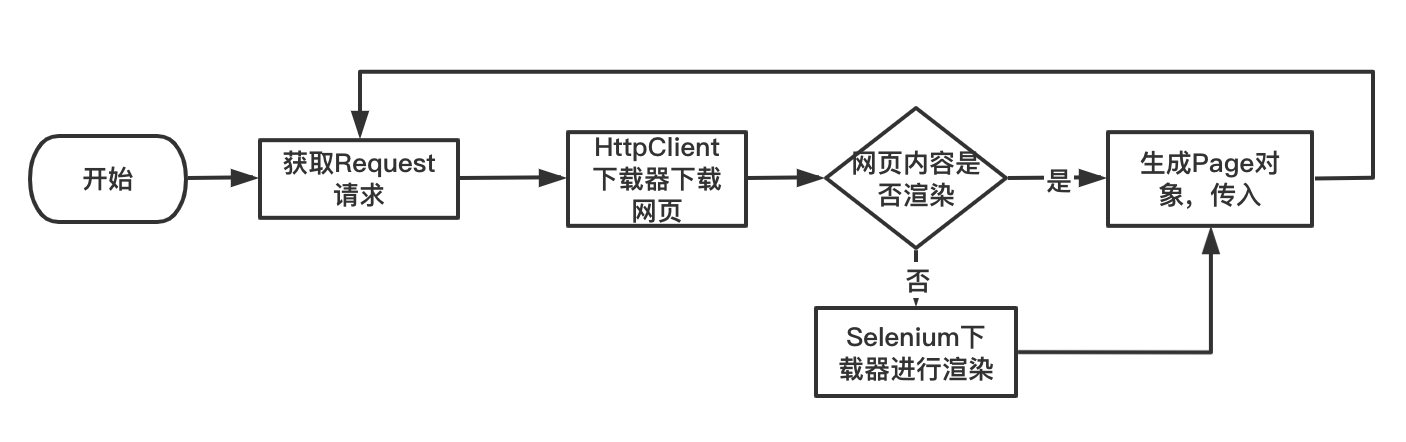
\includegraphics[width=1\textwidth]{pic/downloader.png}
\caption{下载器下载流程}\label{pic:downloader}
\end{figure}

同样地,下载器组件也提供相应的扩展接口,能够自定义下载行为。例如:可以实现通过网络请求的形式将页面下载渲染的任务交给远程浏览器进行渲染,将浏览器和爬虫程序
给分离开来,渲染行为操作直接交给远程浏览器进行,减轻了爬虫过程浏览器渲染的开销,同时还能动态地水平扩展远程浏览器的负载能力。


\subsubsection{链接提取组件}
链接提取是爬虫流程的一个重要过程,其目的是从网页中抽取那些要被跟进的链接。如流程图\ref{fig:link} 所示,获取TargetUrl注解,其中的属性定义了匹配链接的正则表达式,链接提取组件会将
网页上的链接全部提取处理,并进行正则匹配,然后将提取处理的链接封装成Request数据流,异步倒入到Init组件生成的数据流中。
上述流程是链接提取组件的默认实现,当正则匹配无法完全地解析出目标链接时,例如这样一个场景:后续链接的生成并不是靠网页上的链接进行相应的拼接得到的,而是根据
网页上某些文本以及网站链接的规律来生成,框架允许扩展链接提取组件,通过重写链接提取方法,实现用户自定义链接提取逻辑。


\begin{figure}
\centering
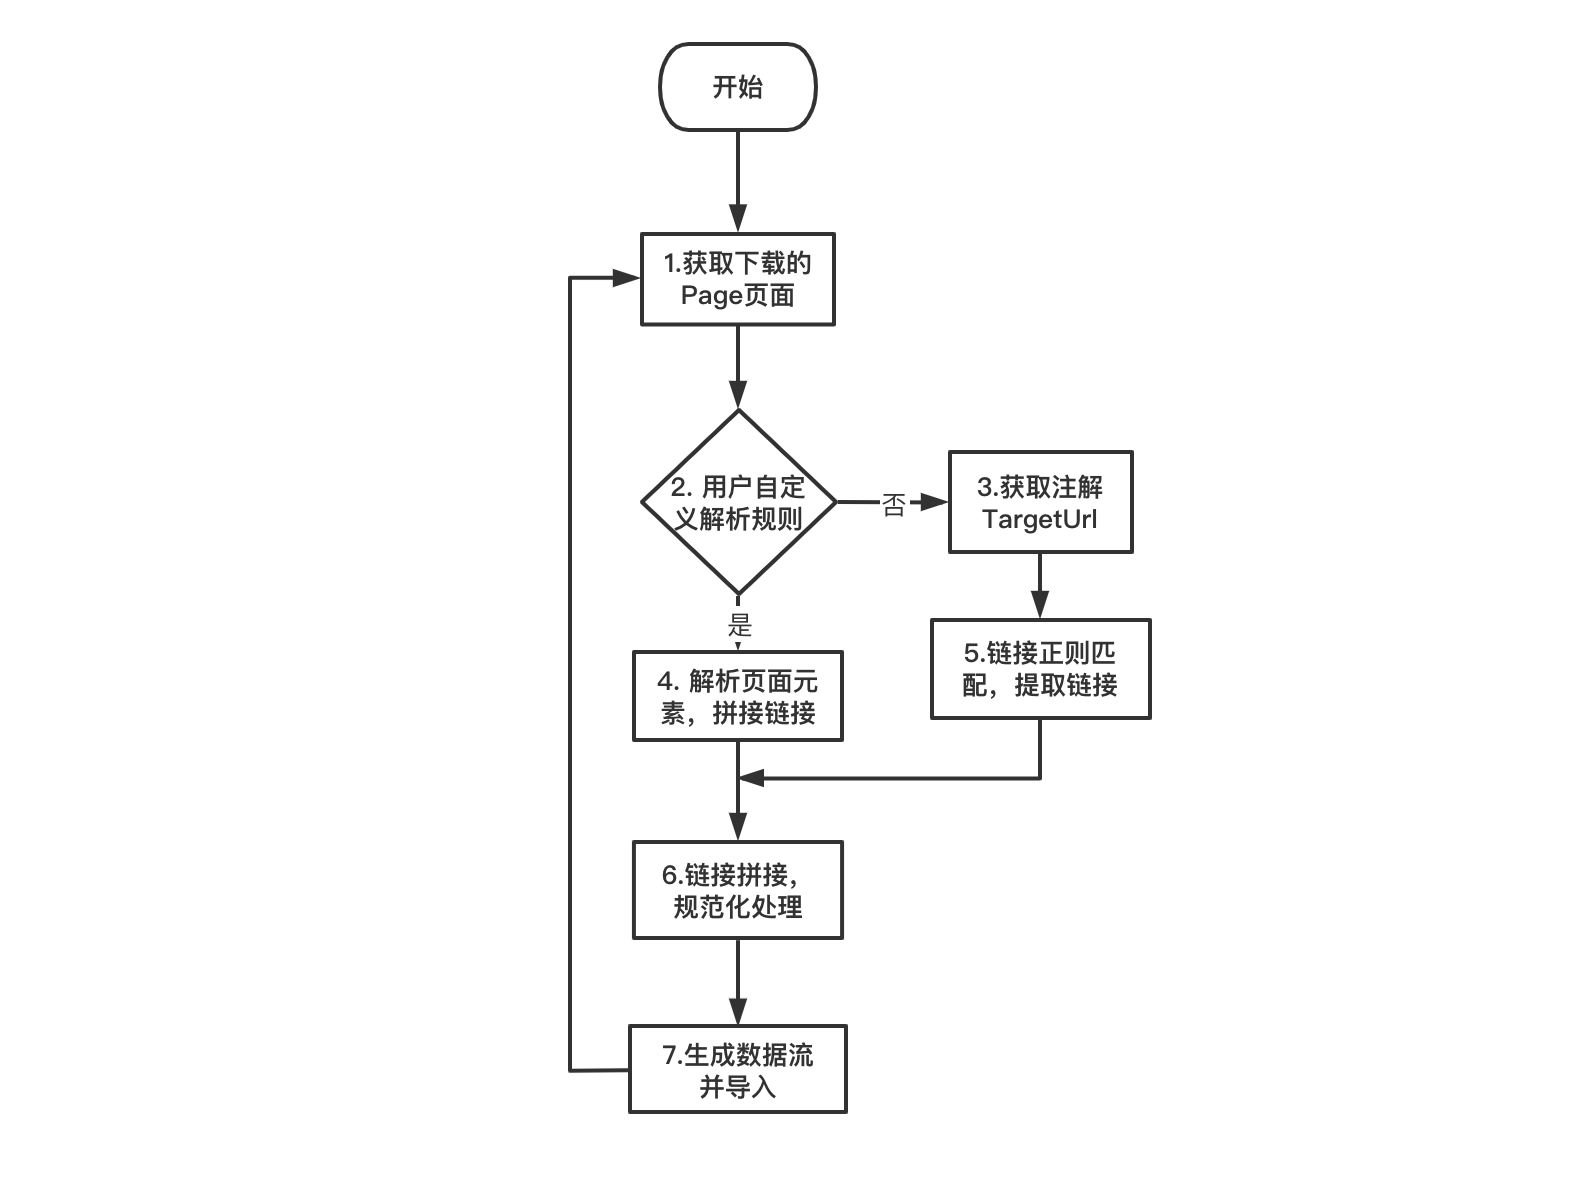
\includegraphics[width=1\textwidth]{pic/linkExtract.png}
\caption{链接提取流程}\label{fig:link}
\end{figure}

\subsubsection{对象映射组件}
对象映射组件是将获取到的网络页面给映射到具体的对象中,将网页上对应的数据装填到对象实例中。通过对象映射组件,将
网页上的数据转换成了结构化或者半结构化的数据,方便后续组件的处理。

对象映射的过程实质上是页面内容解析的过程,通过上文提到的Selector注解来提供映射关系。如图\ref{fig:reflect} 所示,
具体的流程可以描述为:

\begin{enumerate}
  \item[1.] 从上游组件中获取推送的Page对象,Page中包括了整个网页的HTML,对象映射组件主要是对HTML进行相应的解析,获取其中的数据。
  \item[2.] 实例化数据对象,首先调用数据对象的默认构造函数,对对象进行实例化。
  \item[3.] 如果没有自定义解析规则,那么根据Selector注解属性,提取其中定义的CSS选择器来定位页面元素,提取出元素内容。
  \item[4.] 如果有自定义解析规则,则根据自定义规则对HTML页面进行解析匹配。
  \item[5.] 将提取的内容进行类型转换,匹配数据对象中定义的属性类型,然后装填对象实例。
  \item[6.] 将处理好的对象传输到下游组件进行处理。然后转1开始处理下一个Page对象。
\end{enumerate}


\begin{figure}
\centering
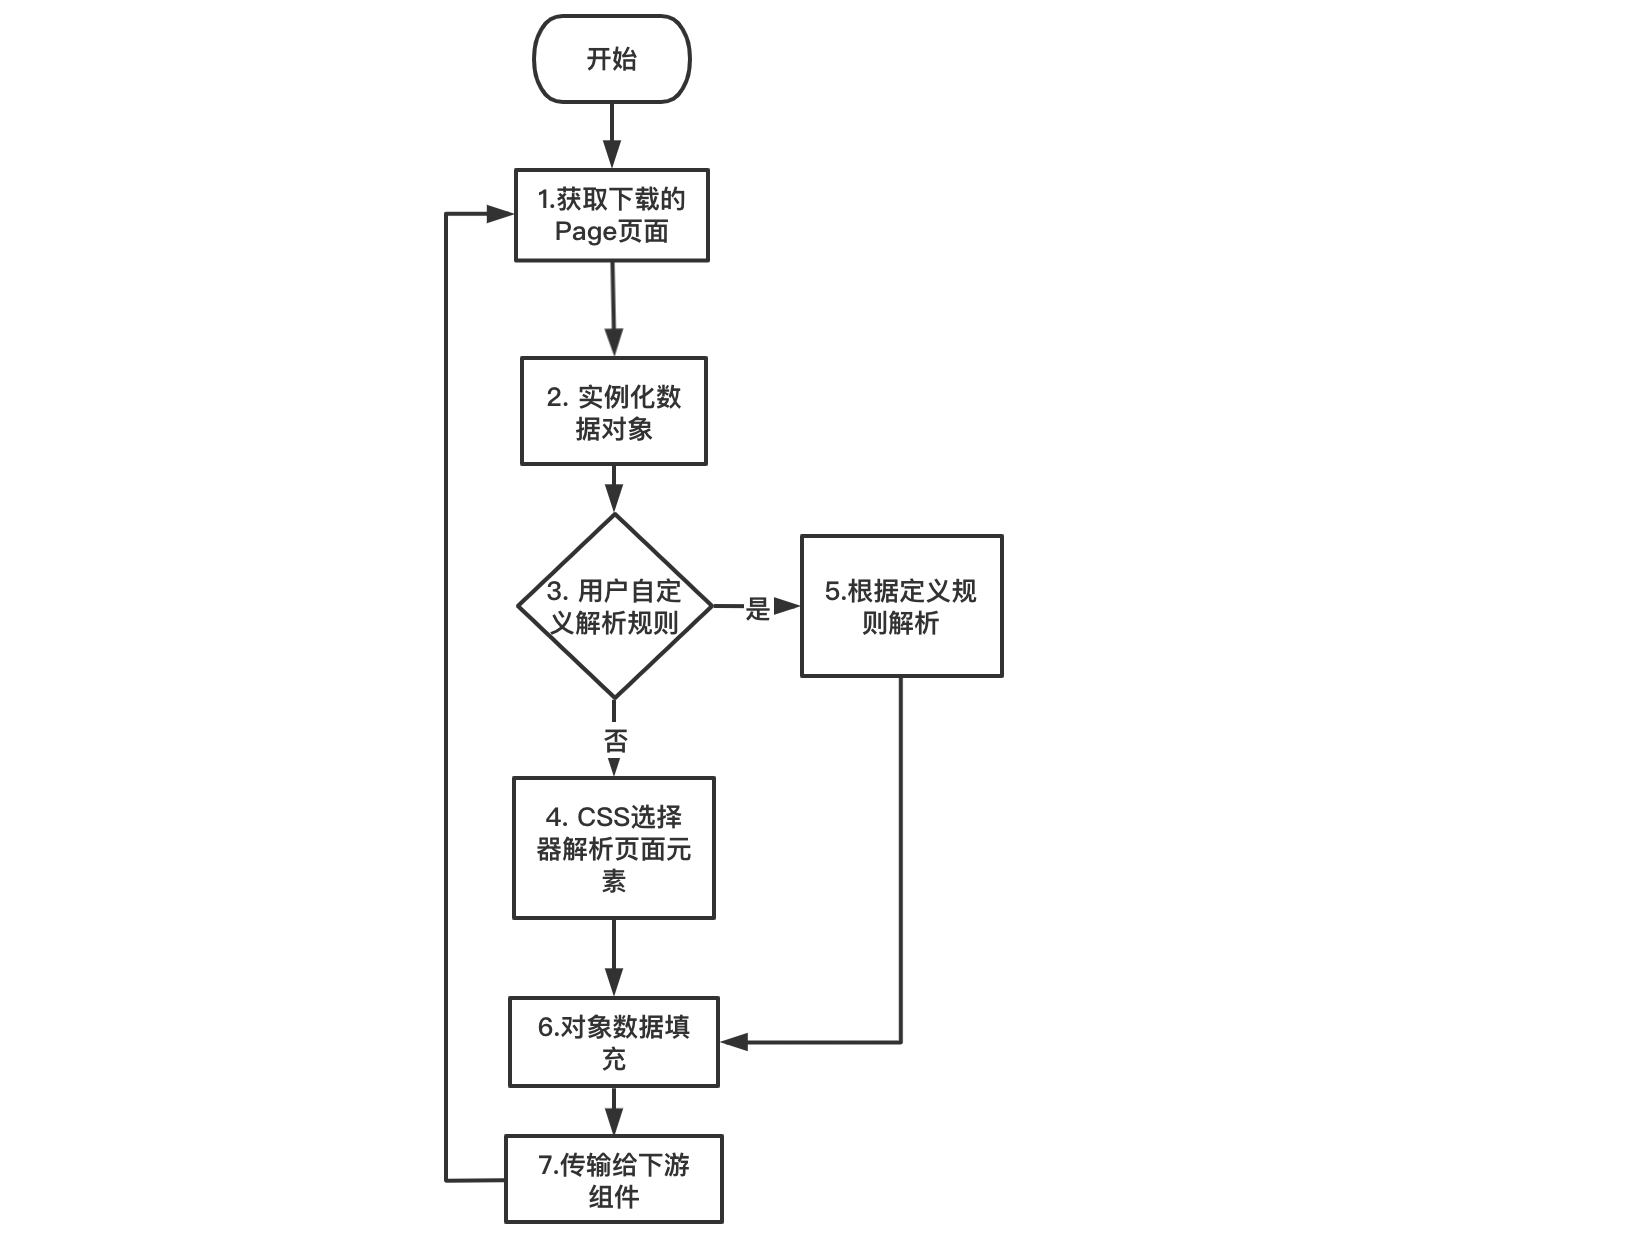
\includegraphics[width=1.2\textwidth]{pic/reflect.png}
\caption{对象映射流程}\label{fig:reflect}
\end{figure}

\subsubsection{扩展组件}
扩展组件是基于Operator接口进行扩展,实现组件逻辑。扩展组件可以存在于整个爬虫流程Init组件之后的每一个阶段,可以存在于下载器组件
和链接提取组件之间,也可以位于过滤组件之后。可以根据编排需要,将扩展组件放置在任意一个位置。

Spidereact通过扩展组件可以实现内容去重,前文提到的过滤组件只是在链接的基础上的去重,如果更进一步处理,可以在映射组件之后加入通过扩展组件实现的内容去重
组件。同样地,Spidereact可以实现持久化存储组件,将结构化的数据存储到数据库中。


\subsection{流程的编排}

流程的编排主要分成三个部分,第一部分是初始化数据流部分(Source),第二部分是对数据的转换操作(Transformation),最后是将转换的
结果输出到一个目的地(Sink)。初始化数据流部分是通过Init组件来实现,数据的转换操作则是由前文提到爬虫的一系列基本组件实现,最后的
结果输出会通过Subscriber订阅者来处理,前两部分构成了一个数据流的发布者,最后通过发布者订阅者模式来对数据的最终处理。

通过编排会形成如图\ref{fig:manage} 所示的逻辑视图。该图展示了一个普通的爬虫程序中,数据在不同的
组件间流动的情况。每个圆圈表示组件,圆圈间的箭头表示数据流,数据流经过不同的组件的处理,最后生成结果到Sink。其中Spidereact通过Init()、
Filter()、Downloader()、Parser()、Transformer()等方法将组件编排到爬取流程OperatorFlow中。各个组件中的处理操作有可能是阻塞的或是
非阻塞的,为了能够构建统一的异步非阻塞处理流,Spidereact编排阶段会对阻塞的组件给分配隔离的异步工作线程池进行处理,将阻塞代码转化成了非阻塞模式
运行,使得爬虫流程中每一部分都是非阻塞处理。

\begin{figure}
\centering
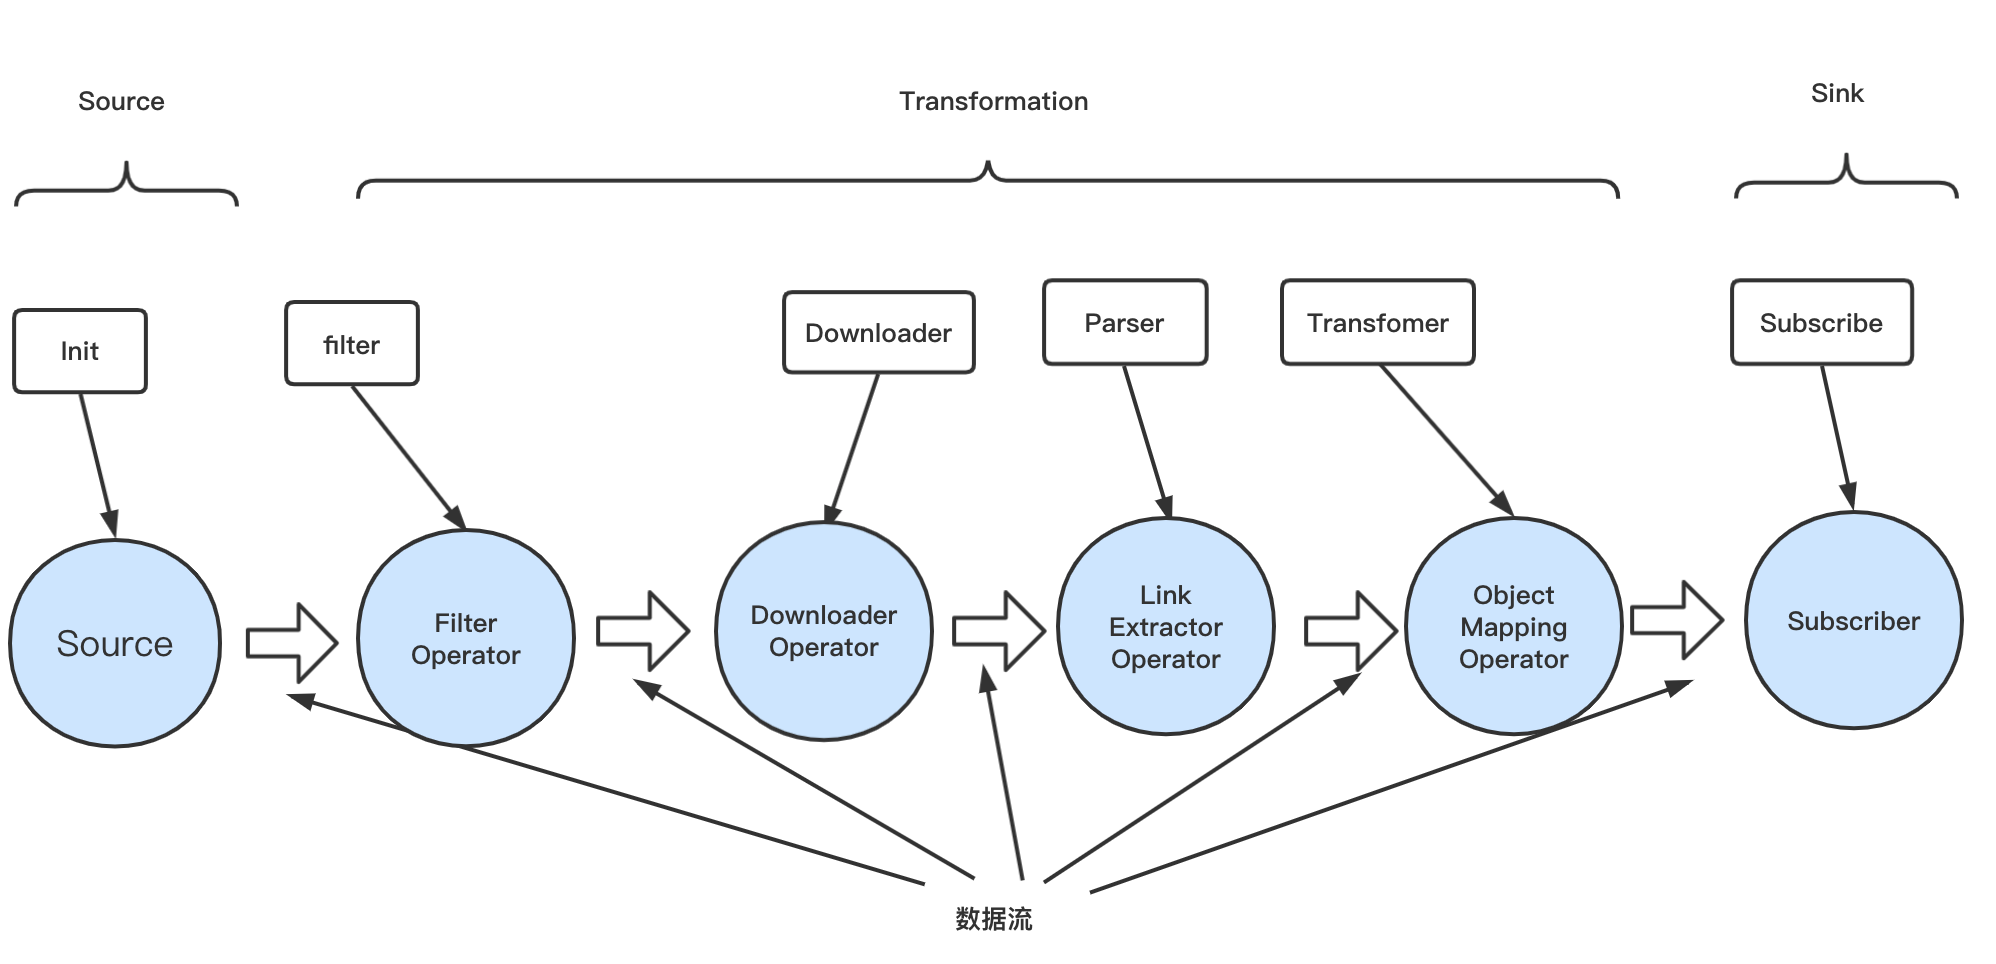
\includegraphics[width=0.98\textwidth]{pic/manage.png}
\caption{流程编排逻辑视图}\label{fig:manage}
\end{figure}

% 除了基本的爬虫流程,我们可以根据需要编排不同的处理流程。例如对于IP代理的实现,我们通过在原有流程中加入IP代理组件,将代理IP整合到Request数据流中,
% 同样地,我们可以构建User Agent流来配置Request流,通过自定义一个UserAgent流生成组件,配置在爬取流程图中下载器之前的阶段,对Request数据流来进行
% 配置。对于登录验证流程,我们可以通过构建Cookie数据流,来对Request流进行配置,同样是在下载器组件之前配置,这样使得请求能够成功响应。后面会详细介绍
% Request数据流的配置。

% \section{爬虫编程模型}



\subsection{异常处理模块}
异常处理模块用以管理Spidereact爬取期间上整个爬虫链路上的异常情况。异常处理模块会捕获所有在各个
组件执行期间引发的异常,并对异常加以处理,使得异常信号不再向下传播。传统多线程编程模型无法捕获
另一个线程中抛出的异常,只能在每个线程内部通过try-catch语句分别处理,或是使用异常处理器UncaughtExceptionHandler来进行
异常处理。但这两种方法都不够优雅,Spidereact通过Project Reactor库对受检异常进行封装并重新传播,
使得异常处理程序能够在下游及时捕捉,并加以处理。

为了管理组件异常,Spidereact自定义了一组异常类型来描述不同组件的异常情况,同时扩展了异常处理接口,能够让用户自定义
异常处理逻辑。如表\ref{table:exception} 所示,Spidereact通过这些Exception类型封装了各个组件处理数据流时遇到的异常,不必在
组件的处理逻辑中对异常进行捕获处理,而是将异常重新抛出,让下游的异常处理程序对异常进行处理。

\begin{table}
\centering
\begin{tabular}{|c|c|}
\hline
异常类型 & 描述 \\
\hline
PageDownloadException & 页面下载时出现的page页面无法下载异常 \\
LinkExtractException & 页面链接无法提取异常 \\
InitException & 初始化Request数据流异常 \\
HtmlToPojoException & 数据映射时出现的数据不匹配异常 \\
\hline
\end{tabular}
\caption{自定义异常类型}\label{table:exception}
\end{table}
如异常处理流程图\ref{fig:error} 所示,异常处理通过hook模式来监听各个组件的运行状况,当某个组件有异常事件抛出时,hook会截获该异常并加以处理。
异常处理过程类似于事件监听机制,整个爬虫是基于异步消息驱动,会将异常作为消息信号向下游传播,若下游未定义异常处理,那么整个爬取流程将会终止。

\begin{figure}
\centering
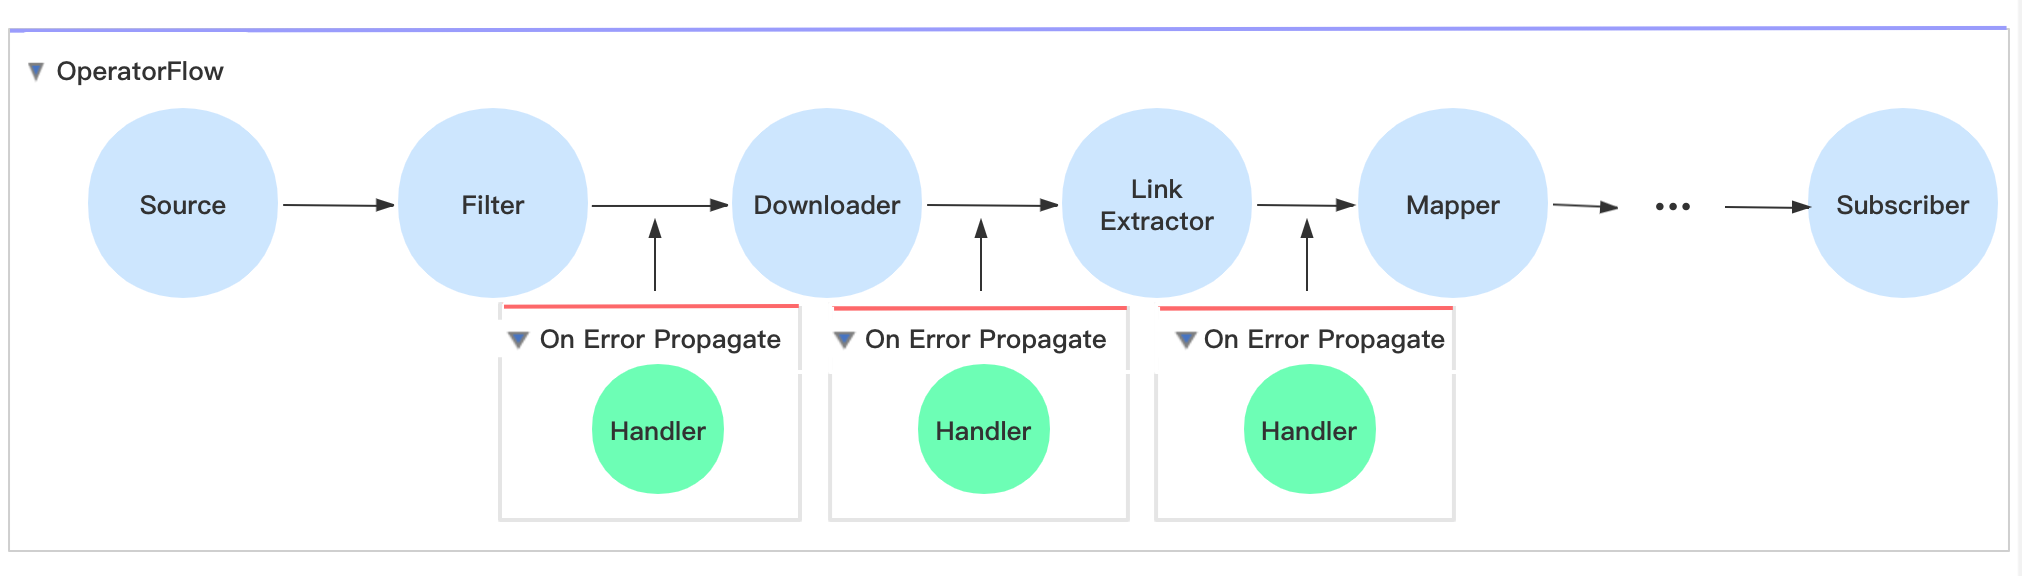
\includegraphics[width=1\textwidth]{pic/error-handling.png}
\caption{异常处理流程图}\label{fig:error}
\end{figure}
当爬取流程正常运行时,数据流从source出发,途径filter、downloader、linkExtactor等等,最后被subsriber消费。但当某个组件处理数据时出现异常情况,
该组件会将异常抛出,异常也被是当作一个信号,和正常的数据信号一样会向下游传播。该异常会被自定义的handler给截获,触发异常处理程序进行处理,整个异常处理
流程并不会影响到爬取的正常处理流程。

\subsection{监控模块}
监控模块用来通知和收集爬虫数据,通常是通过键值对的形式来统计数据,其中的值往往是计数器。
Spidereact实现了StatsCollector来对数据进行收集,并且提供了相关API方便访问。

StatsCollector收集器会收集以下信息:
\begin{enumerate}
  \item 总共爬取的网页数量:所有的请求总数。
  \item 当前正在爬取的网页数量:目前下载器中正在处理的网页数量。
  \item 成功爬取的网页数量:成功解析到数据的页面数量。
  \item 爬取失败次数:在爬取的任一节点失败的次数总量。
  \item 爬取速率:爬取成功页面数量除以时间。
  \item 请求等待数量:目前正在等待下载器处理的请求数量。
  \item 各组件处理时间:数据流经每个组件需要的处理时间。
  \item 各组件处理数量:各个组件各自处理的数据总量。
  \item 各组件吞吐量:各个组件单位时间内处理的数据数量。
  \item 端到端平均处理时间:从source组件出发到数据最后被消费所平均花费的总时间。
\end{enumerate}

通过统计这些信息来实时监控一个爬取流程,在爬取时可以实时获取,有助于检测爬虫状态。

开发者可以通过继承StatsCollector来自定义爬虫数据收集逻辑,通过定义相关指标,来实时观察
爬虫过程中指标的变化。

\subsection{Web模块}
Web模块主要是对Spring对整合,将Spidereact中的实例加载为Spring Bean,从而使得开发者能够
结合Spring框架中使用Spidereact获取网络数据。


为了能够被Spring加载成Bean,Spidereact定义了2个基础注解:
\begin{enumerate}
  \item Operator: Operator注解用来标识会被Spring加载对组件,同时注解属性中通过index还定义了组件在爬取流程图中的相对位置,方便OperatorFlow的构建。
  \item OperatorScan: OperatorScan注解用来描述组件所在的包,Spring容器在加载Bean的过程中,会通过OperatorScan对包目录下的所有Operator注解标识的组件进行加载。
\end{enumerate}

如图\ref{fig:webuml} 所示, InitializingBean接口是由Spring框架提供的,可自定义初始化Bean。当Spring容器启动后,会对SpiderreactAutoConfiguration进行加载,
同时将OperatorFlowAwarePostProcessor加载,之后OperatorScanRegistrar会扫描所有的Operator组件,构造OperatorFlow,并将OperatorFlow传入到FlowController中。
应用通过FlowController来获取爬虫爬取的结果数据流加以处理。

\begin{figure}
\centering
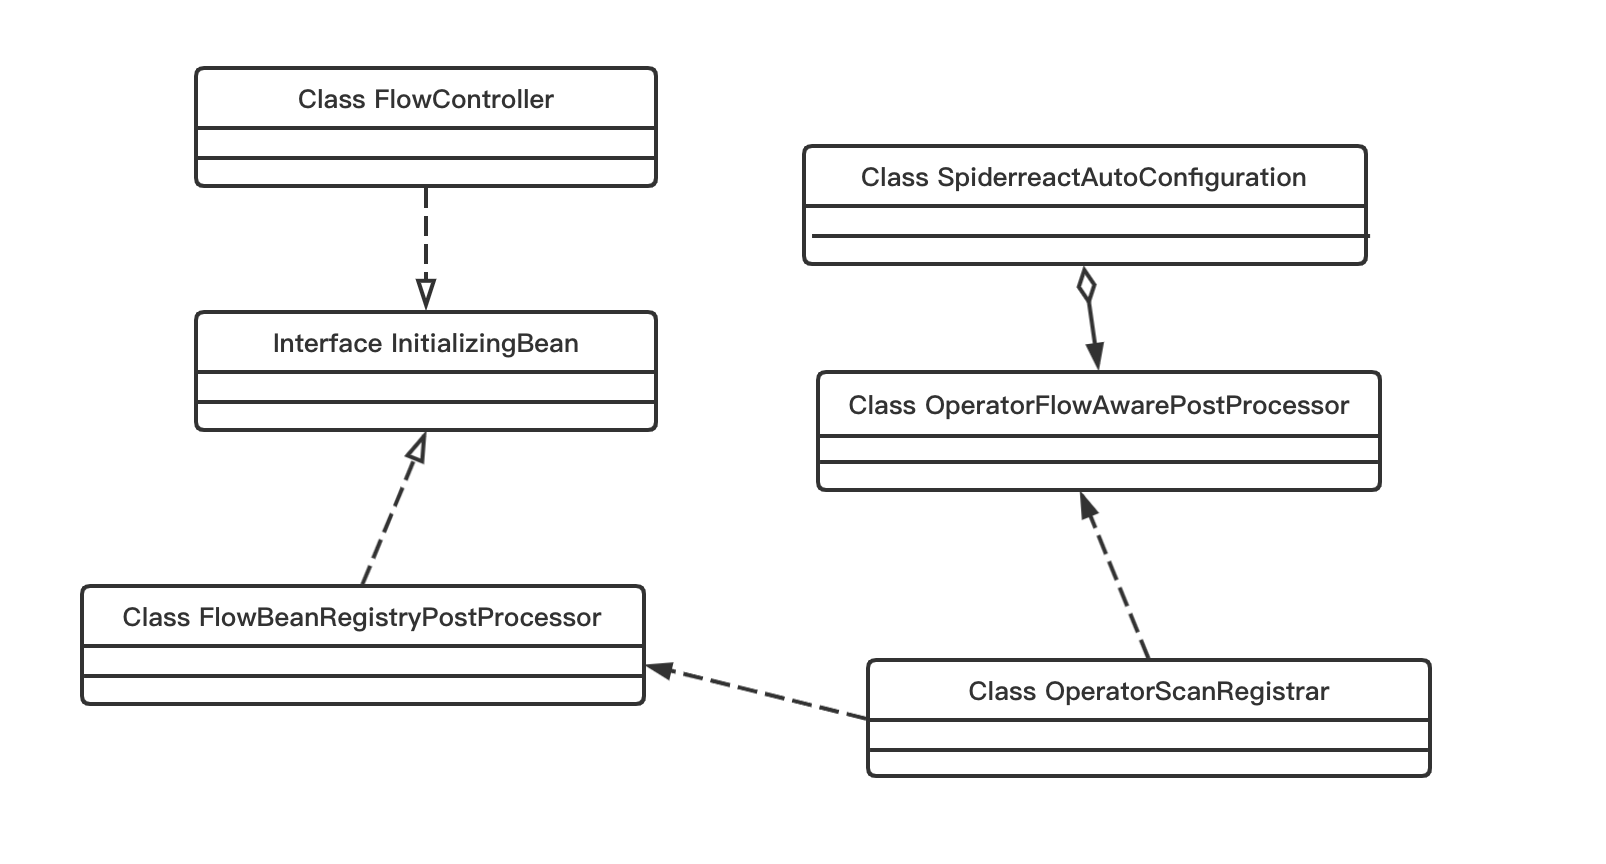
\includegraphics[width=0.98\textwidth]{pic/webuml.png}
\caption{Web模块UML类图}\label{fig:webuml}
\end{figure}

\section{Spidereact爬虫开发}
下面通过介绍Spidereact爬虫开发过程,包括爬虫数据对象定义和爬取流程编排,后面还有关于
爬虫反爬策略的设置。
\subsection{数据对象定义}
Spidereact爬虫开发需要根据爬虫的经验知识,以及对网页数据结构和网站链接结构的了解,来对爬取的数据模型进行建模。爬虫数据模型既需要描述对象属性,
还需要描述数据模型与网络结构的映射关系,将网页结构数据与数据模型进行关联。

如代码\ref{code:all} 所示,通过StartUrls描述爬取起点,InnerUrl以及TargetUrl描述爬取链接的跟进策略,通过两者的描述来构建网页爬取遍历的层次树状结构。
然后通过Selector中的CSS选择器进行页面元素和对象数据的映射。
\begin{lstlisting}[label = code:all, caption = {数据模型定义}]
@StartUrls(values = "http://www.example.com")
@InnerUrl(value = "")
@TargetUrl(value = "")
public class Doc {
    @Selector(value = "")
    String title;

    @Selector(value = "")
    String text;

    @Selector(value = "")
    String comments;

    public String toString(){
        return "{ " + title + ", " + text + ", " + comments + " }";
    }

}
\end{lstlisting}

\subsection{组件定义}
首先是Init组件,如代码\ref{code:init} 所示,通过继承SourceOperator来定义了初始化组件。
由于初始化组件已经有了默认实现,开发者只需要指定泛型类型即可。
\begin{lstlisting}[label = code:init, caption = {Init组件定义}]
public class Init extends SourceOperator<Doc> {
}
\end{lstlisting}

过滤组件默认实现是DuplicateFilter,同时爬虫开发者还可以通过重写组件来自定义组件逻辑,如代码\ref{code:filter} 所示,通过Filter组件重写了Reqeust重复过滤组件。
\begin{lstlisting}[label = code:filter, caption = {Filter组件定义}]
public class Filter extends DuplicateFilter<Request> {
  
    @Override
    public Boolean process(Request source, OperatorContext context) {
        // some code
        xxxxx;
    }
}
\end{lstlisting}

爬虫的下载器组件也有默认实现类DefaultDownloader,链接提取组件的默认实现则是DefaultPageProcessor类。

接着是对象映射组件组件,如代码\ref{code:map} 所示,通过继承HtmlToPojoAdapter来定义了映射组件。
\begin{lstlisting}[label = code:map, caption = {映射组件定义}]
public class HtmlToPojo extends HtmlToPojoAdapter<Doc> {
}
\end{lstlisting}


\subsection{爬虫编排}

爬虫通过OperatroFlow来编排管理各个组件,通过fluent编程风格来创建了一个流式爬虫。如代码\ref{code:manage} 所示,爬虫
通过编排Init、Filter、Downloader等组件类,便构建了Spidereact爬虫。同时,开发者根据subscribe方法对爬虫生成的结构化的流式数据进行处理。
\begin{lstlisting}[language=Java, label = code:manage, caption = {爬虫编排}]
flow.init(Init.class)
    .filter(Filter.class)
    .downloader(DefaultDownloader.class)
    .parser(DefaultPageProcessor.class)
    .transformer(HtmlToPojo.class)
    .build()
    .subscribe();
\end{lstlisting}

\subsection{爬虫反反爬策略配置}
下面本文通过一个例子来介绍Spidereact的反反爬策略配置。
\begin{lstlisting}[label = code:anti, caption = {爬虫反反爬策略配置}]
\\ 代理IP、User Agent、Cookies切换间隔分别为2000ms、3000ms、10000ms
Flux<Proxy> proxyFlux = ProxyProvider.setSwitchInterval(2000)
    .generateFlux();
Flux<String> userAgentFlux = UserAgentProvider.setSwitchInterval(3000).generateFlux();
Flux<Cookies> cookiesFlux = CookiesProvider.setSwitchInterval(10000).generateFlux();
flow.init(Init.class)
    .delayElements(Duration.ofMillis(100))
    .zipWith(proxyFlux)
    .zipWith(userAgentFlux)
    .zipWith(cookiesFlux)
    .filter(Filter.class)
    .downloader(DefaultDownloader.class)
    .onErrorContinue(error -> Mono.empty())
    .parser(DefaultPageProcessor.class)
    .transformer(HtmlToPojo.class)
    .build()
    .subscribe();
\end{lstlisting}

正如上一章\ref{section-anti} 所诉,Spidereact可以通过不同的配置流对Reqeust流进行配置。如代码\ref{code:anti} 所示,proxyFlux、userAgentFlux以及cookiesFlux分别
配置了不同的切换时间间隔。Reqeust数据流经过一段固定时间的爬取后,其相应的代理IP、User Agent以及请求的Cookies会进行切换,以此来绕过网站设置的反爬措施。
同时Spidereact通过delayElements来设置爬虫请求的延迟,以及通过onErrorContinue算子来处理各个爬虫组件数据处理过程中的异常。

\section{本章小结}
本章对于结合Reactive Programming的流式爬虫方法的设计与实现进行了描述。首先对框架的整体编程模型进行了介绍,并和传统
爬虫框架的多线程编程模型进行了对比。然后介绍了爬虫的几个基本组件以及扩展组件的设计,阐述了各个组件的功能。接着对框架的
各个模块进行了介绍。

下一章则是实验设计与评估,验证框架的有效性。



%%%%%%%%%%%%%%%%%%%%%%%%%%%%%%%%%%%%%%%%
%%%%%%%%%%%%%%%%%%%%%%%%%%%%%%%%%%%%%%%%

\chapter{实验设计与评估}\label{Chapter_test}
前面章节介绍了Spidereact的设计与实现,本章则对Spidereact的性能进行评估,通过和当前开源爬虫框架的对比
来验证Spidereact爬虫在资源利用率以及爬取效率方面的提升。



\section{实验内容}
正如前文所诉,Spidereact是为了解决多线程模型爬虫中存在的阻塞IO问题实现的响应式爬虫框架,其目的是提高系统资源的使用率,并提高爬取的效率。
因此实验主要对比Spidereact爬虫在相同的条件下与其他爬虫框架实现的爬虫在CPU利用率以及吞吐量上的差异。同时,还对其他有可能影响
实验结果的因素进行了分析,排除其他因素的干扰。
具体的实验主要对比两个方面:

\begin{itemize}
\item 当资源不受限时,爬虫的爬取效率以及CPU使用率之间的对比。
\item 在相同的资源限制下,爬虫的爬取效率对比。
\end{itemize}

\section{实验设置}

\begin{table}
\centering
\begin{tabular}{|l|c|r|}
\hline
硬件类型&型号&数量(大小) \\
\hline
CPU&Intel(R) Xeon(R) CPU E31265L @ 2.40GHz&4核 \\
内存& TEAMGROUP-SD3-1600 DDR3&16G \\
网卡& Intel Corporation 82579LM&1Gps \\
磁盘& C400-MTFDDAT064M & 60G \\
\hline
\end{tabular}
\caption{硬件配置}\label{hardware_config}
\end{table}

\begin{table}
\centering
\begin{tabular}{|l|c|}
\hline
名称 & 软件版本 \\
\hline
操作系统 & Linux ubuntu 4.4.0-186-generic \\
容器引擎 & Docker 18.09.7 \\
Java & OpenJDK 1.8 \\
\hline
\end{tabular}
\caption{软件环境}\label{software_config}
\end{table}

\subsection{实验环境}
% 我们是基于Java实现了Spidereact,
实验主要的硬件和软件环境如表\ref{hardware_config} 和表\ref{software_config} 所示,
实验运行在3台服务器上,每台服务器上都有一块四核CPU,并且都采用了超线程技术,每台服务器有8个逻辑处理器。

\subsection{实验对象}
对于爬虫性能的测试,实验参考了Scrapy框架Benchmark测试的方法\cite{thalheim2004website},它通过生成本地的HTTP服务器,通过Scrapy爬虫配置最快的速度进行网页爬取,从而来测试
Scrapy框架在本地硬件的具体表现,来获得一个通用的比较标准。
实验需要模拟搭建一个虚拟网站,其中网站能够模拟现实环境中的网站,即发送请求后,经过一段时间延迟后,返回响应结果。
搭建的模拟网站返回的是Apache Tomcat的文档,这些文档页面都是静态页面,网站总共1230个页面。为了尽量地爬取多个页面,比较性能,实验并未设置
爬虫的重复URL过滤,意味着爬虫仍然会爬取已经爬取过的页面。

\subsubsection{网站模拟与压测实验}
模拟网站跑在两台服务器上,通过Nginx进行负载均衡,使得网站能够尽可能地承受更大的负载,而不至于随着爬虫程序请求量的增加而崩溃。
同时我们对网站进行了压测实验,确保了网站自身因素不会影响爬虫测试的效果。

我们通过gatling\footnote{https://gatling.io/}{\zhdash}一款基于AKKA\footnote{https://akka.io/} 和Netty\footnote{https://netty.io/}开发的高性能压测工具,对网站进行了压测实验,设定每秒恒定的并发数发送请求,持续100秒时间,查看
网站吞吐量,平均响应时间等指标。

如表\ref{table:pressure-test} 所示,我们发现,随着压测实验访问并发度的提高,网站吞吐量也随着增加,
请求的平均响应时间也在增加,而请求的成功率随之下降,但变化不大,绝大部分请求都能得到响应。
另外在1000并发度的情况下压测,我们仍然可以认定请求依旧可以被成功处理,而且在垂直爬虫的实践中,往往不会对同一个网站有这么大的并发量,
本次爬虫性能测试实验的并发量也不会超过1000。压测实验表明,网站自身的状况不会影响到爬虫程序之间的性能对比。

\begin{table}
\centering
\begin{tabular}{|c|c|c|c|c|c|}
\hline
场景 & 总请求数 & 平均TPS & 成功率 & 平均响应时间(ms) & TP95(ms) \\
\hline
200并发 & 20000 & 200 & 100\% & 27 & 102 \\
\hline
500并发 & 50000 & 413 & 99.2\% & 1371 & 2750 \\
\hline
1000并发 & 100000 & 757 & 89.6\%  & 2102 & 3621 \\
\hline
\end{tabular}
\caption{模拟网站压测}\label{table:pressure-test}
\end{table}

\subsubsection{实验对比框架}
Scrapy是基于事件循环机制的单线程爬虫,通过Twisted框架实现的异步网络通信。Scrapy爬虫运行过程中会启动多个线程,但是爬虫爬取主流程都是跑在单个线程上的,其余的线程
用来处理爬取主流程无关的事情。Scrapy将爬取的主流程是交给Twisted线程池,任务结束后,会发起回调执行回调函数。Scrapy通过CONCURRENT\_REQUESTS参数来控制下载器Downloader的并发,但该参数只是为了控制Downloader最大的并发请求数,并不是爬虫本身的线程并发,CONCURRENT\_REQUESTS只能控制传给Twisted的异步任务数量。换句话说,无论是在CPU单核还是多核环境下,Scrapy爬虫的CPU利用率不会超过100\%,Scrapy爬虫无法利用多核CPU优势来提高
爬虫吞吐量。如图\ref{scrapy} 所示,实验测试了Scrapy爬虫在不同CONCURRENT\_REQUESTS配置下的吞吐量情况。可以看出,随着参数的增大,爬虫的吞吐量并没有显著的增加,一直维持在60/sec上下波动。实验过程中,我们确保Scrapy的Request队列中有足够的待爬取的Request,排除了Request队列待爬取请求数量不足的影响。实验发现不论如何配置Scrapy爬虫的相关参数,Scrapy爬取
的吞吐量基本不会发生太大的变化。实验结果表明,Scrapy爬虫的爬取效率取决于Twisted主线程的处理能力,无法利用CPU多核的优势。

由于Scrapy爬虫的单线程限制,实验无法比较Scrapy爬虫框架与Spidereact在不同并发下的CPU性能以及吞吐量情况。基于这种考虑以及Python运行环境
的因素,本次实验将重点比较Webmagic和Spidereact两个爬虫框架之间不同并发下的性能差异。

实验对比的对象是Spidereact与Webmagic框架,Webmagic框架是基于Java实现的典型的多线程模型网页爬取的爬虫框架,而Spidereact则是基于异步非阻塞的响应式爬虫编程模型
来进行网页爬取的。为了能够对比爬虫框架的优劣,本次实验通过Webmagic和Spidereact开发了针对测试网站的爬虫,并对爬虫的并发度进行不同的配置,
分别比较不同并发度下Spidereact与Webmaigc的具体性能情况。

\begin{figure}
\centering
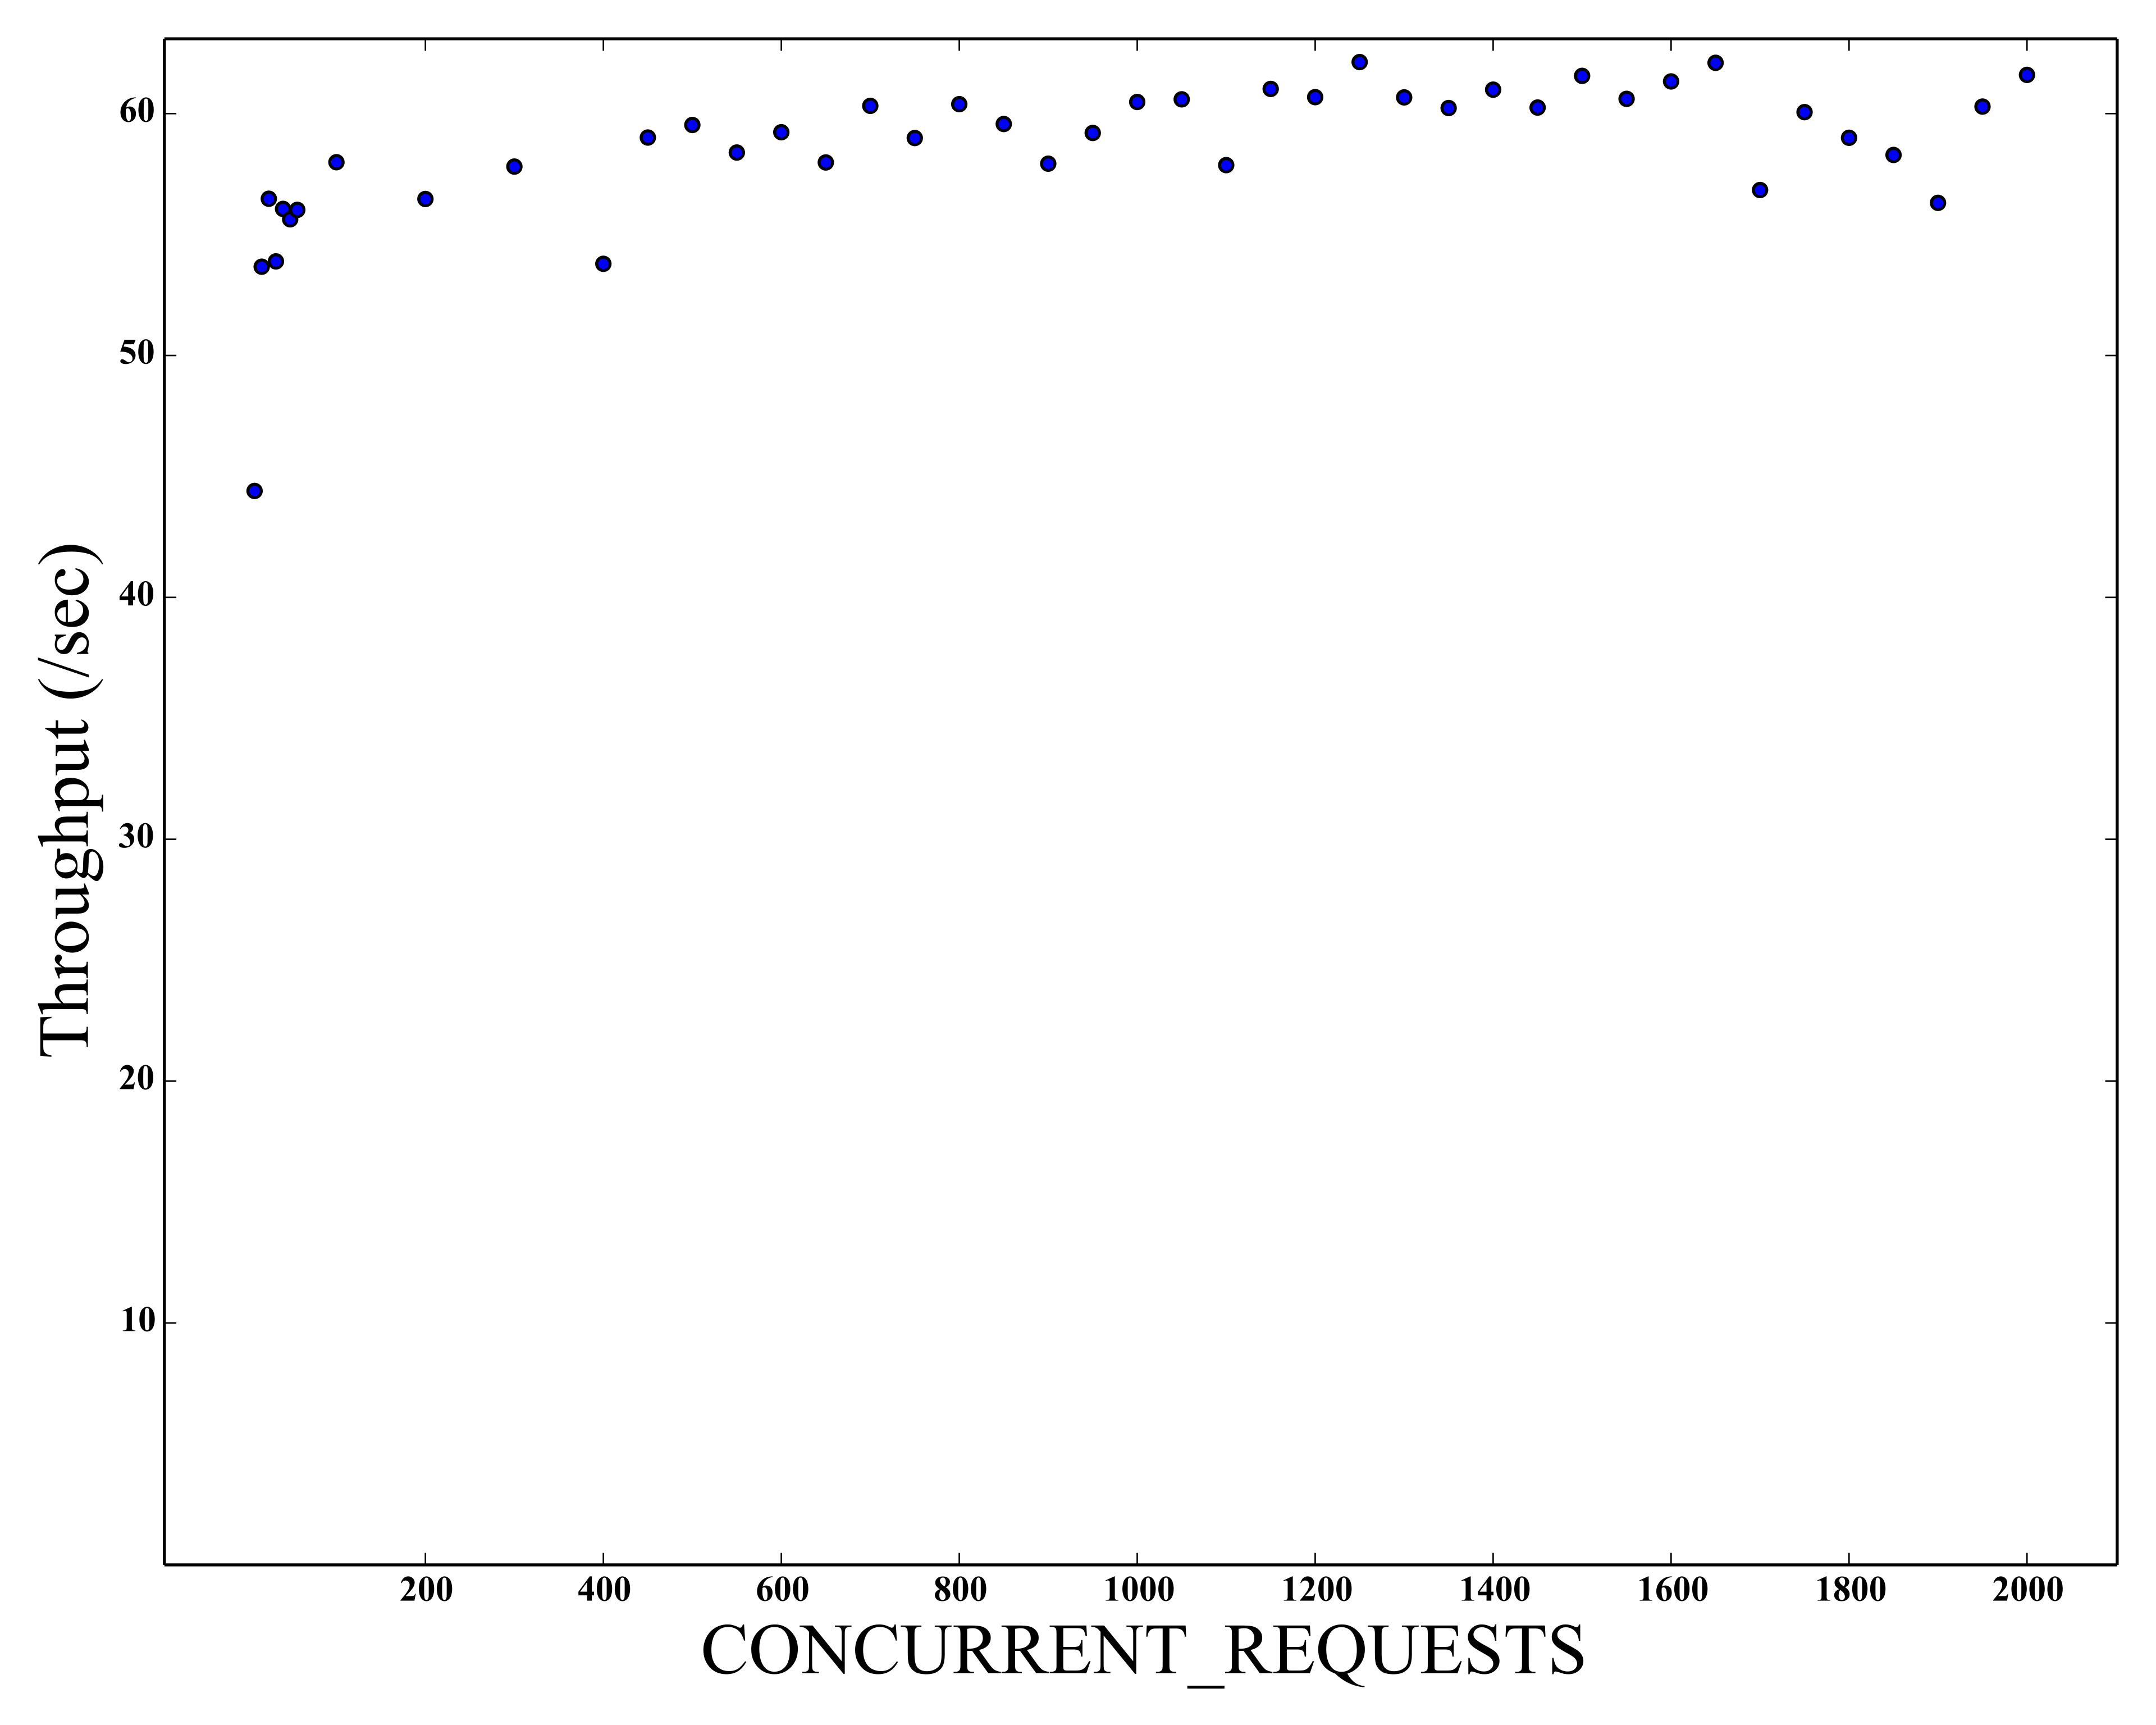
\includegraphics[width=0.8\textwidth]{pic/scrapy.png}

\caption{Scrapy不同CONCURRENT\_REQUESTS配置下吞吐量}\label{scrapy}
\end{figure}

\subsection{模拟延迟}
上面提到的实验是针对一个模拟的静态网站的爬取。与真实网站不同的是,爬虫的请求发送到网站服务器端后,网站能够做出很快的响应。因为模拟网站为静态网站,没有
额外的处理流程,只是将存储的静态网页返回给了爬虫。为了更进一步模拟真实网站爬取,实验通过Linux下的一个流量控制工具tc(traffic control)来控制网站端的发包操作,
tc控制直接对物理网卡生效,将物理网卡的发包时延设置40ms、100ms、200ms来延迟发送,并设置延迟时间有上下10ms的波动,
来模拟真实网站的响应处理延迟。


\section{实验结果与分析}

\subsection{CPU利用率验证}
Spidereact旨在提高爬虫对CPU的利用率,能够有效地利用CPU的计算资源来加快爬取的速度。通过对比Spidereact爬虫与Webmagic爬虫之间的CPU使用率,
来验证Spidereact是否能够提高CPU的利用率。


\begin{figure}[!htbp]
\centering
\subcaptionbox{\footnotesize {100并发}}{
    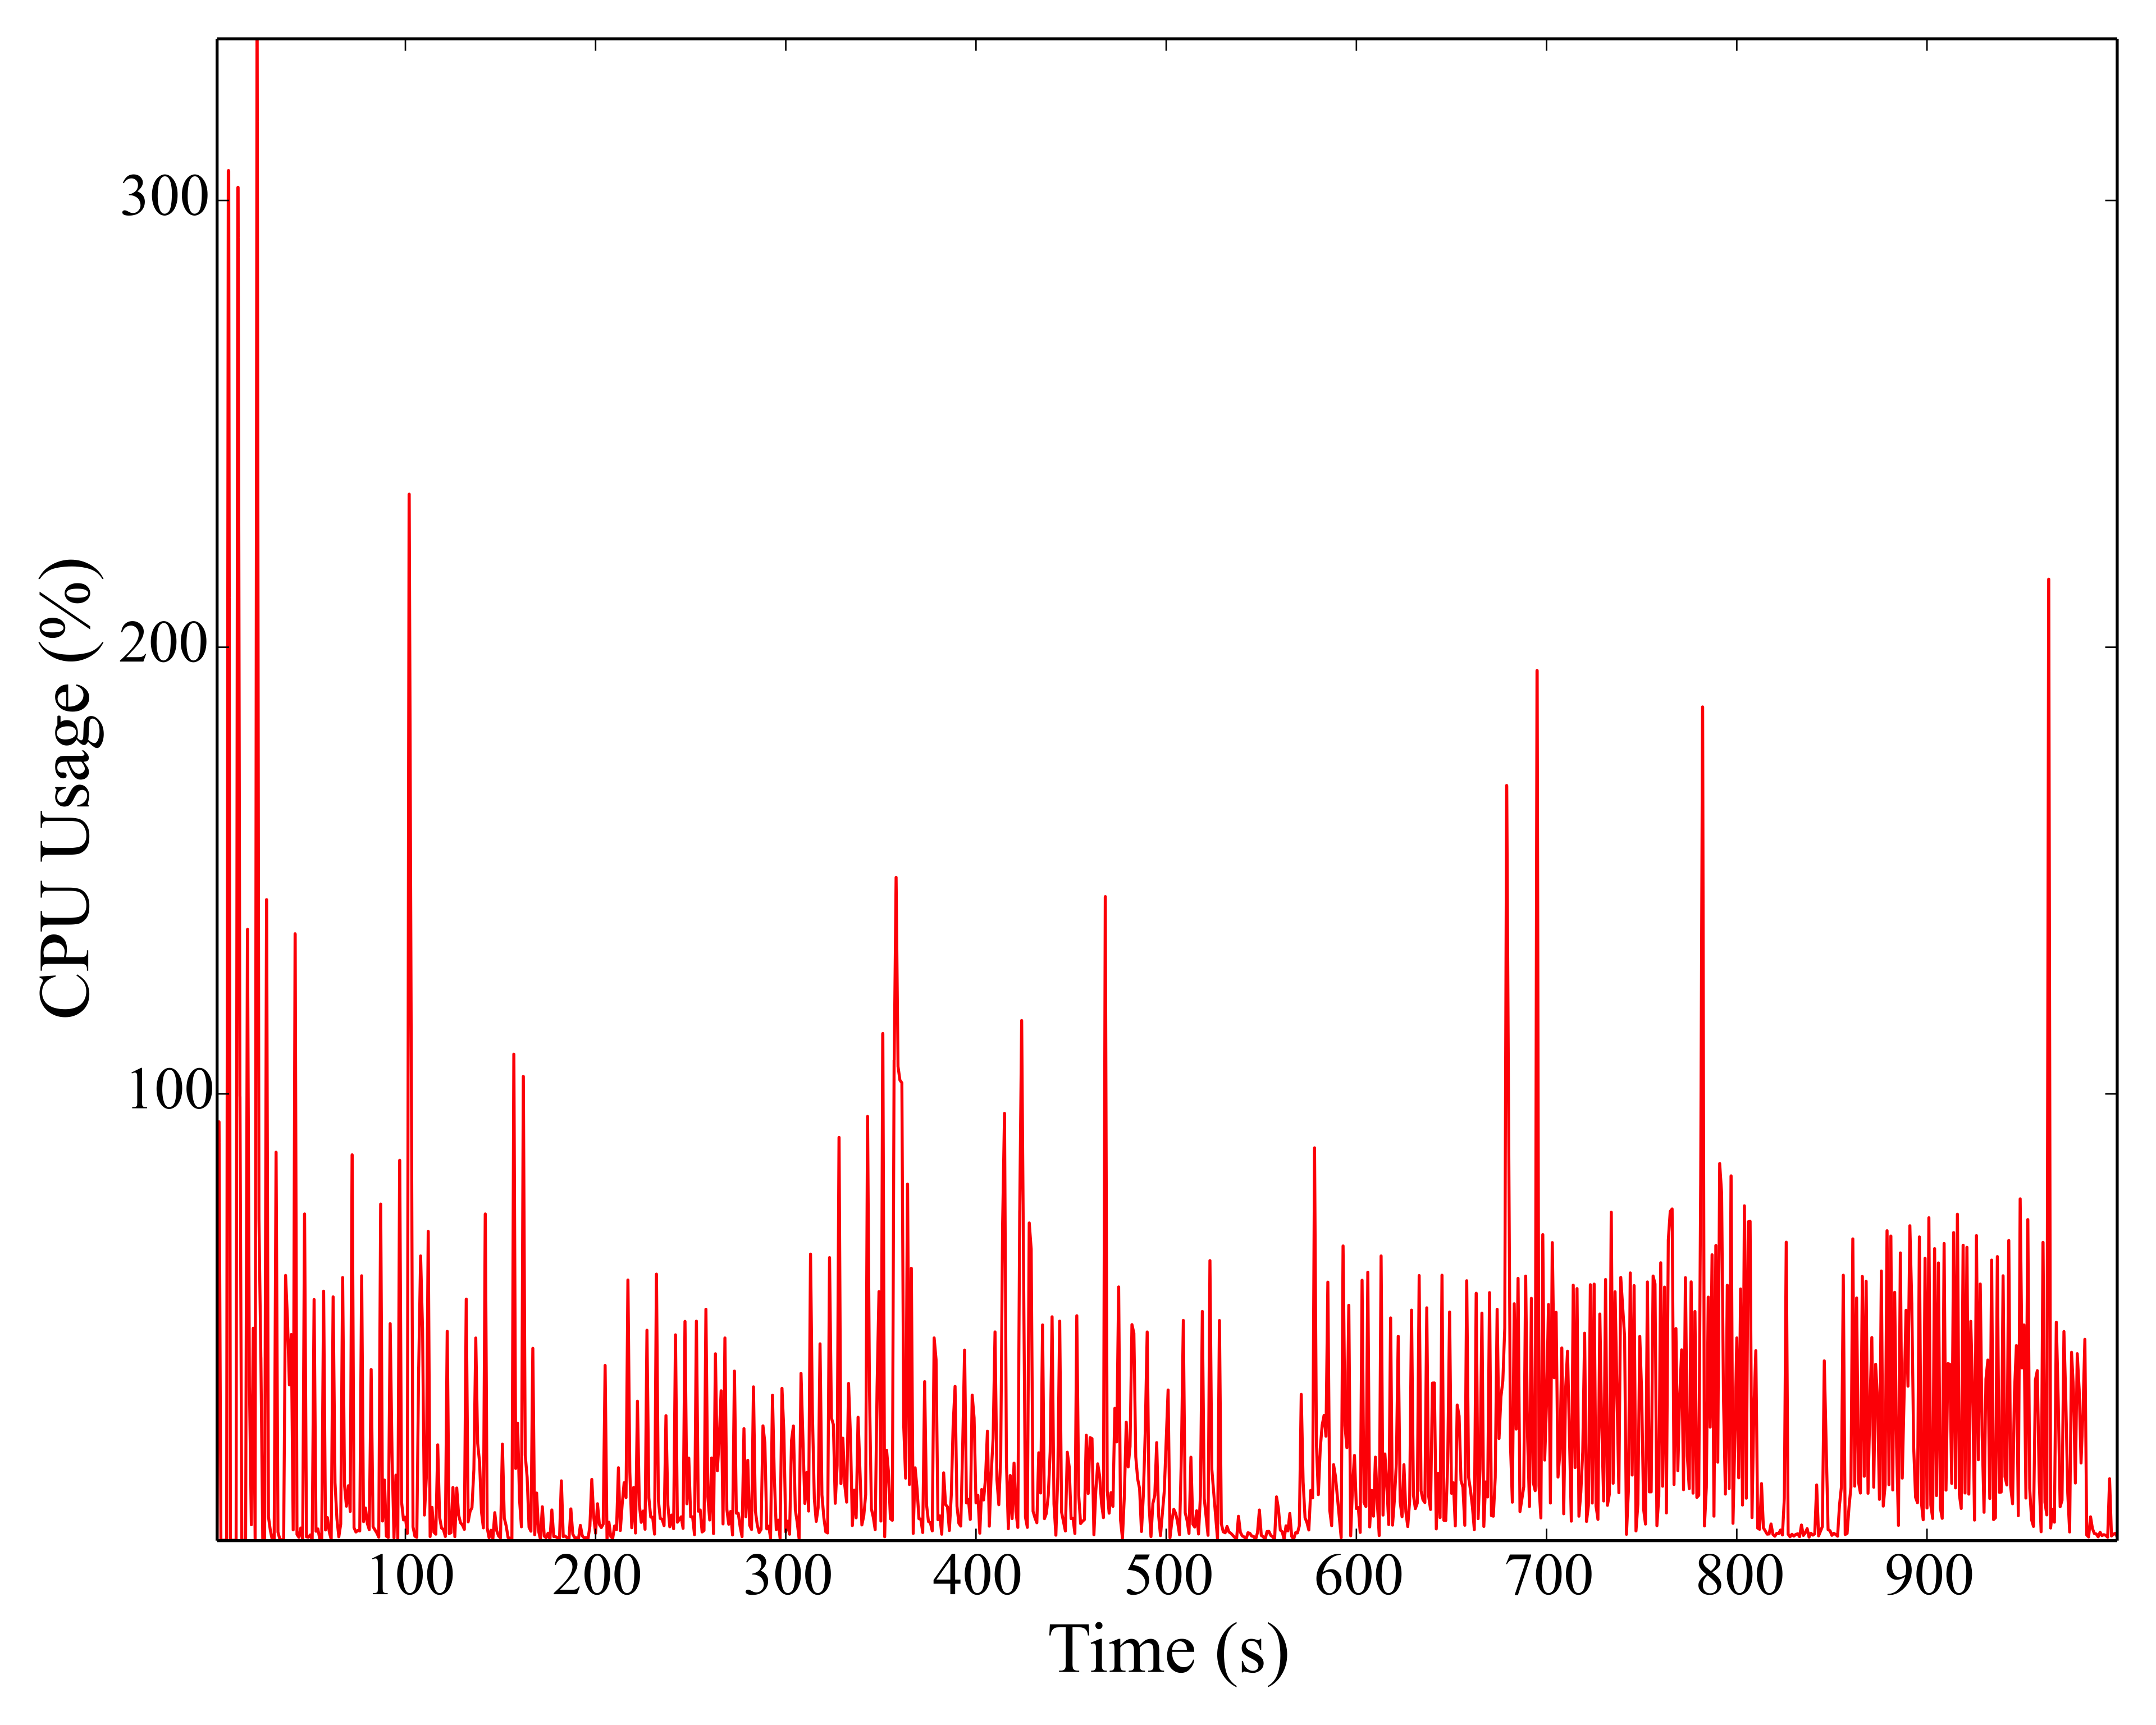
\includegraphics[width=0.45\textwidth]{pic/webmagic0ms100.png}
  }
  \hfill
  \subcaptionbox{\footnotesize {300并发}}{
    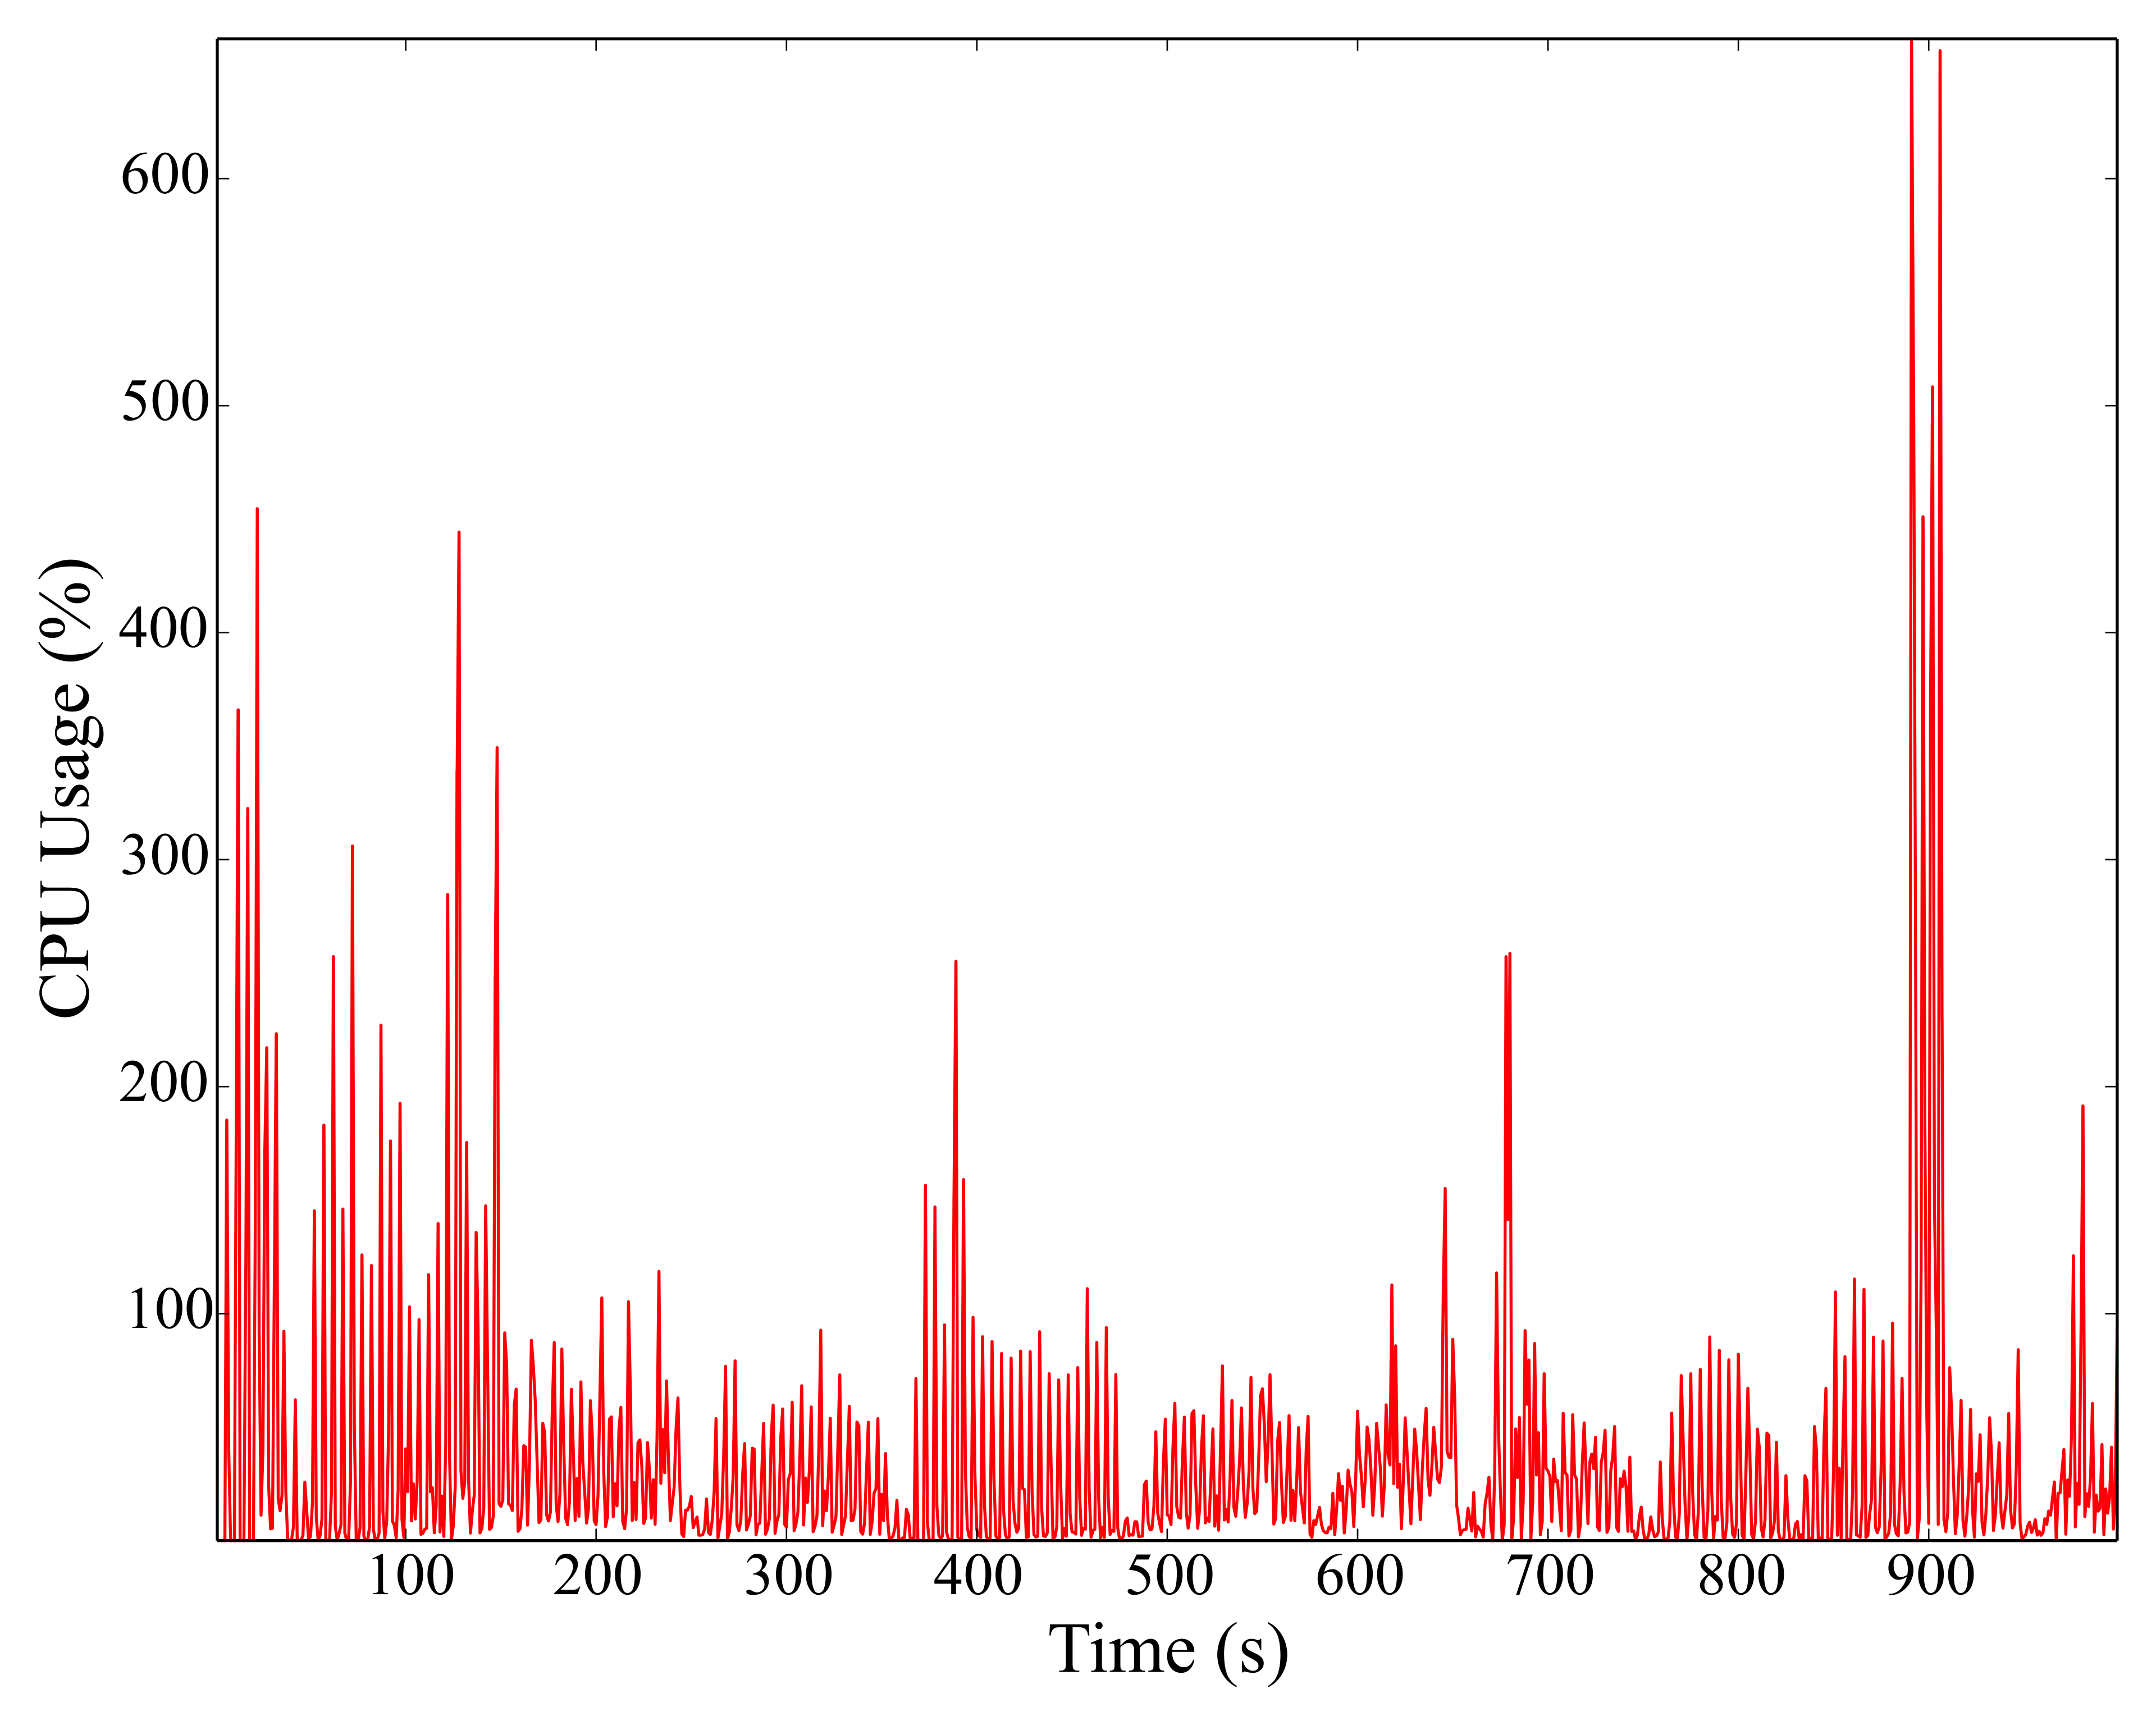
\includegraphics[width=0.45\textwidth]{pic/webmagic0ms300.png}
  }
  \\
  \subcaptionbox{\footnotesize {600并发}}{
    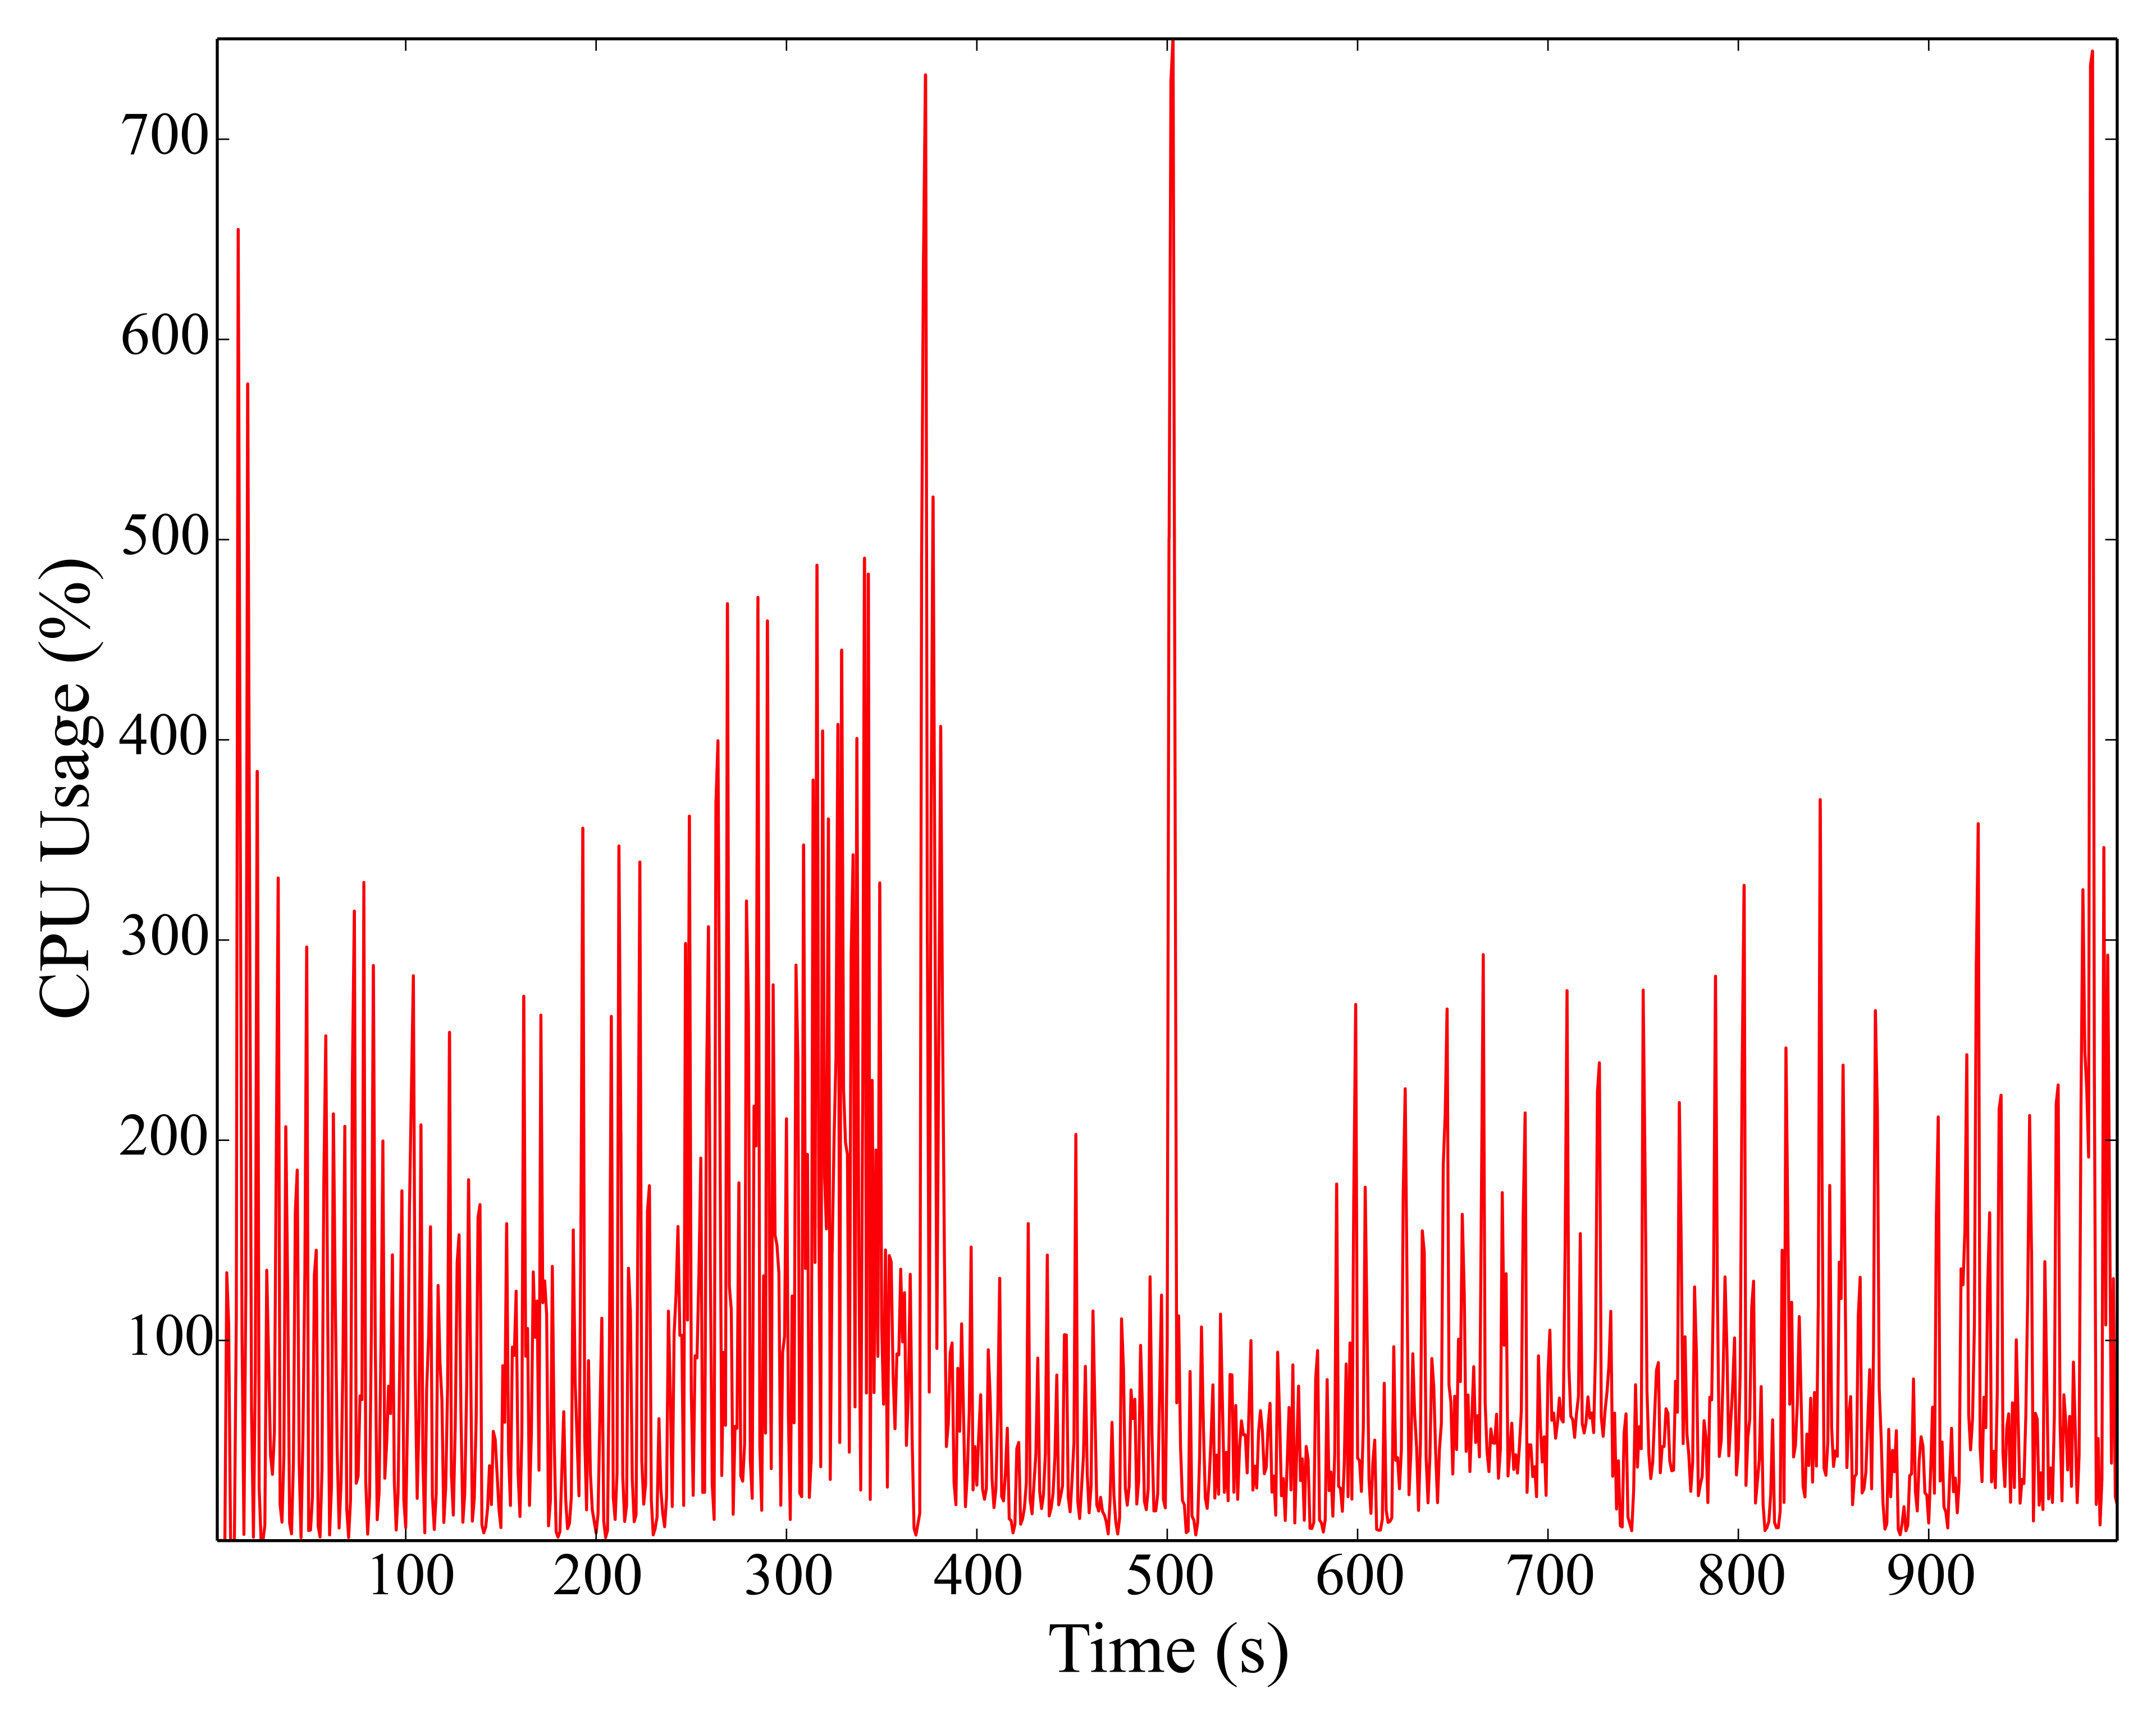
\includegraphics[width=0.45\textwidth]{pic/webmagic0ms600.png}
  }
  \hfill
  \subcaptionbox{\footnotesize {1000并发}}{
    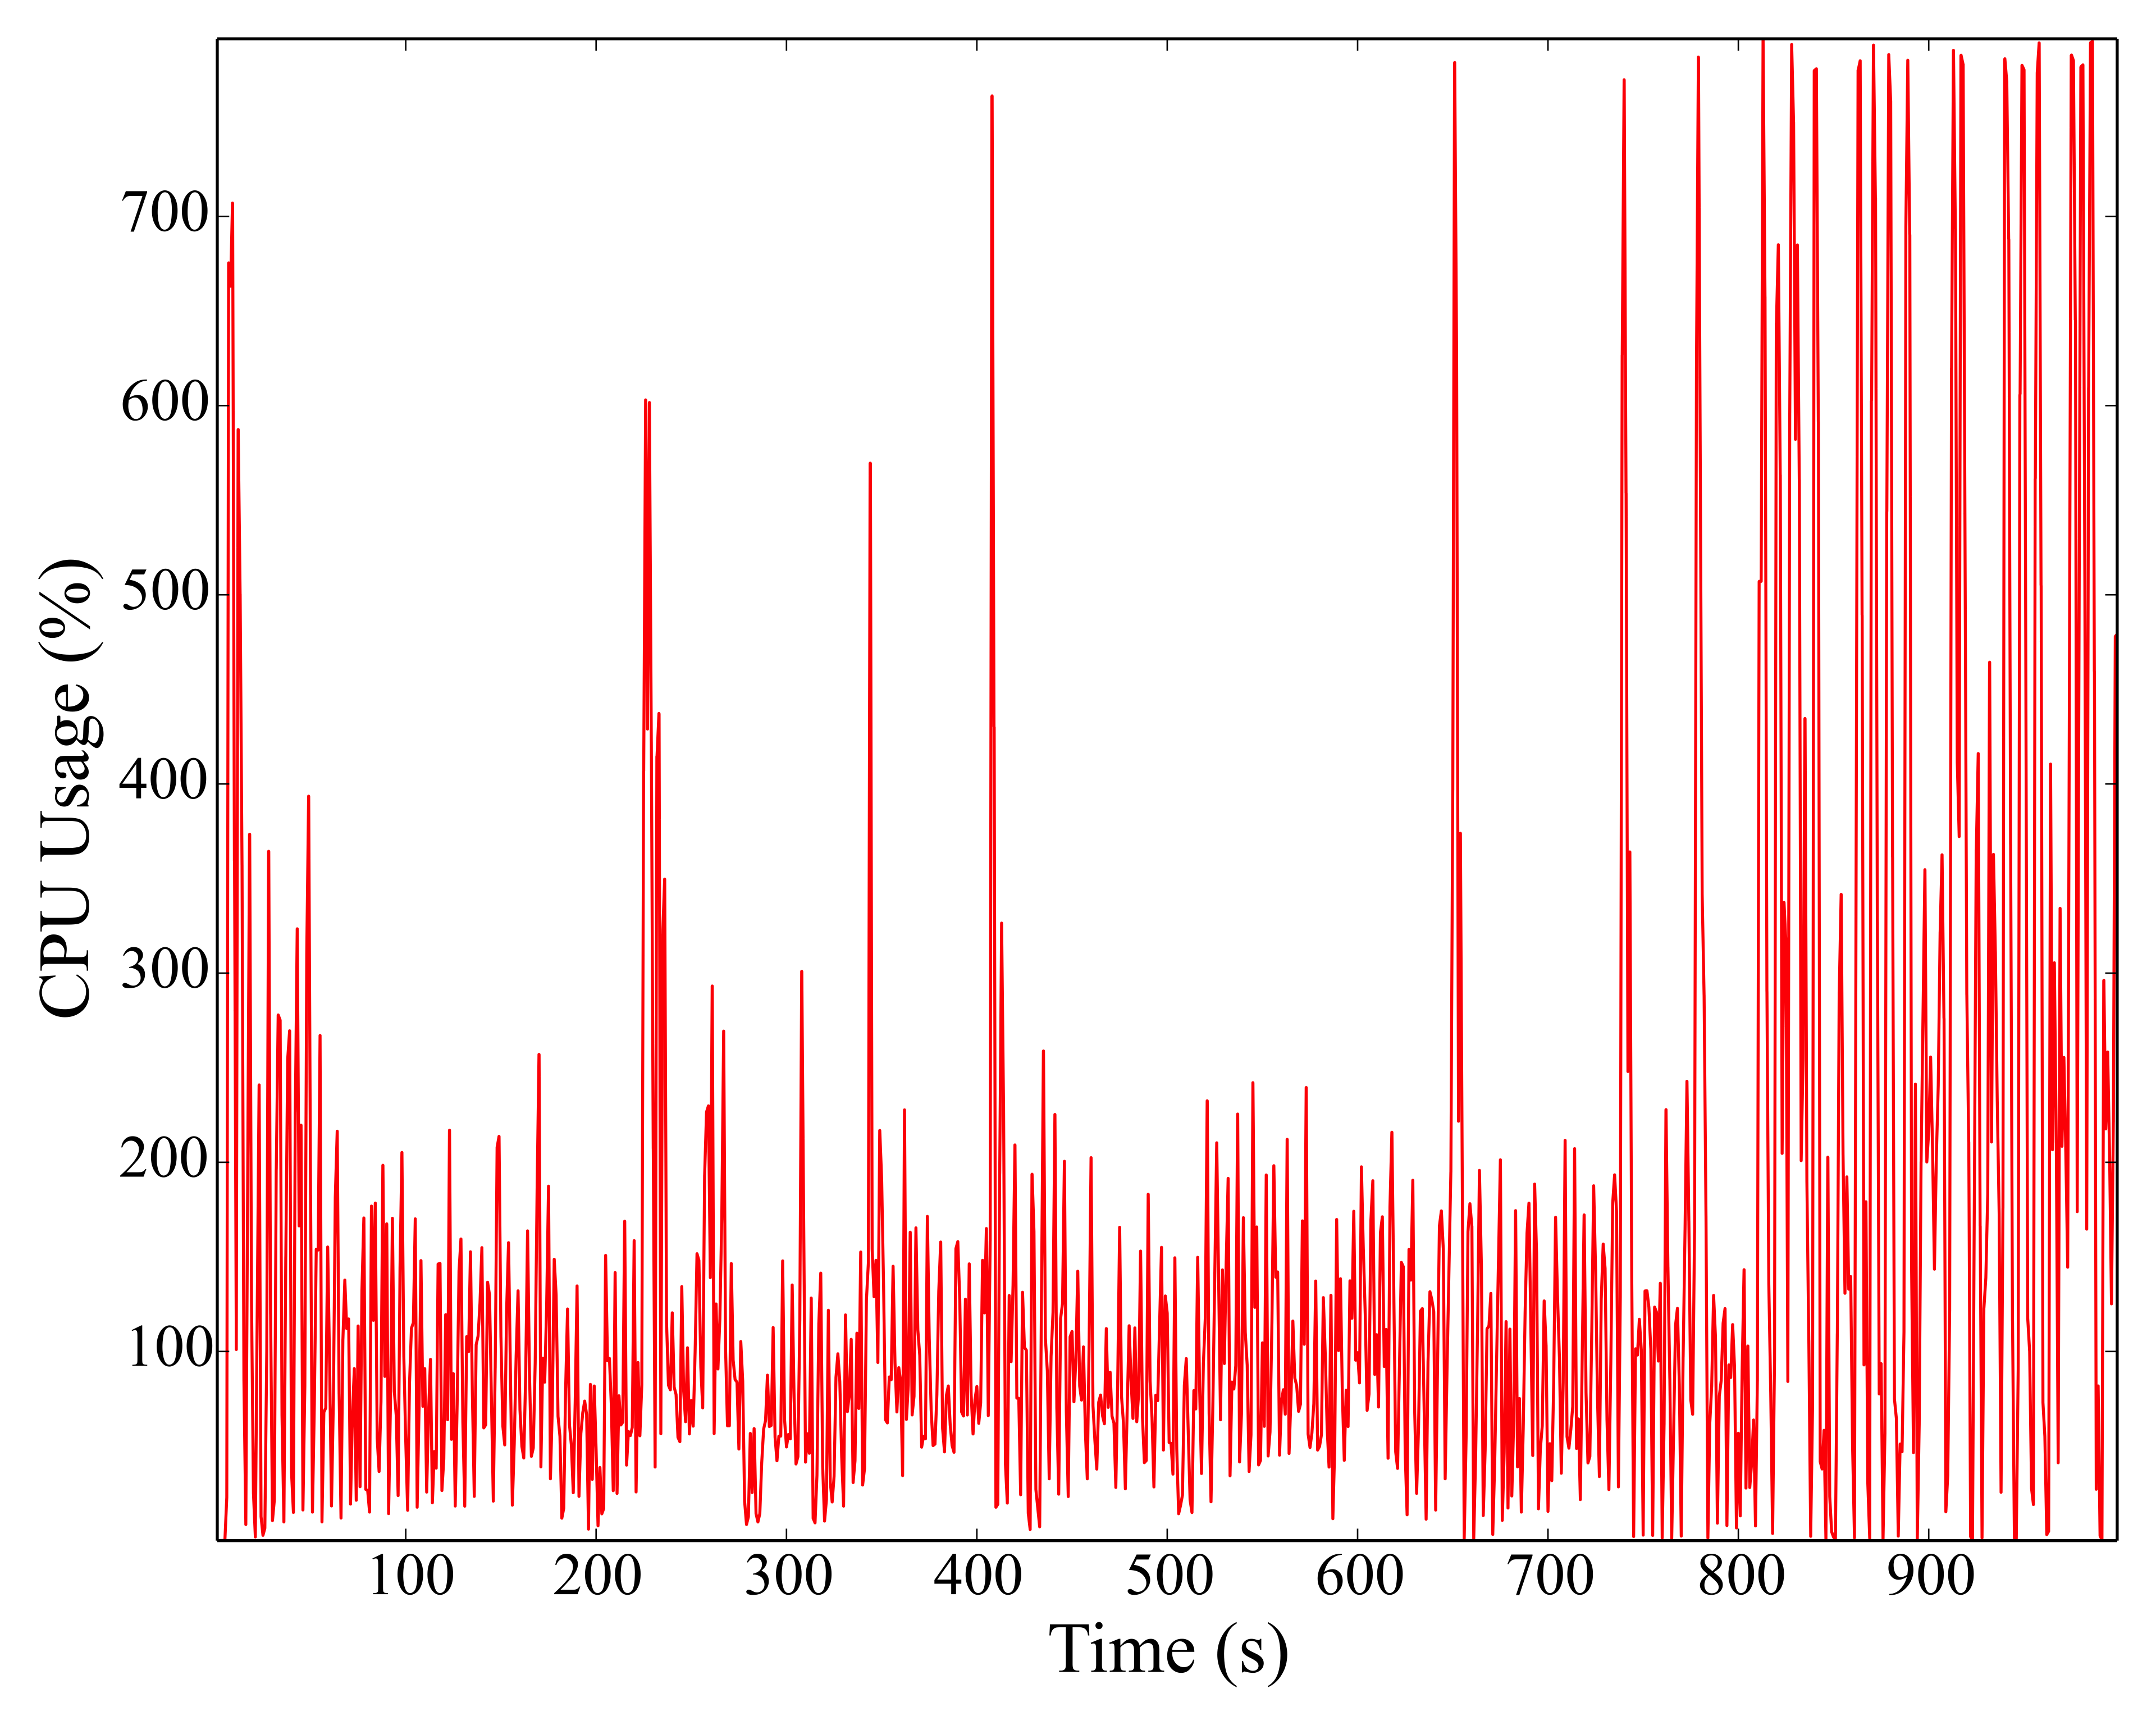
\includegraphics[width=0.45\textwidth]{pic/webmagic0ms1000.png}
  }
\caption{Webmagic 0时延不同并发下CPU使用情况}\label{fig:concurrent}
\end{figure}
爬虫CPU利用率是爬虫进程的CPU时间除以总的CPU时间,进程的CPU时间包括了执行用户态代码占用的时间和执行内核态代码占用的时间。又由于
爬虫是运行在有8个逻辑处理器的服务器上,需要将各个逻辑处理器上的CPU利用率相加。CPU利用率计算公式如下所示,其中$\Delta t$表示进程的
CPU占用时间,$T$表示总CPU时间。

\begin{equation} 
  Usage\% = \sum_{i=1}^n \frac{\Delta t}{T}
\end{equation}

实验基于Docker环境来对爬虫进行资源的限制,首先在无资源限制的条件下对Webmagic和Spidereact进行实验对比。
从图\ref{fig:concurrent} 中我们可以发现,Webmagic在0ms时延\footnote{0ms时延是指并未设置模拟延迟,并不是说不存在网络时延}情况下不同并发度的CPU利用率情况。可以发现,在不同并发度下,Webmagic的CPU利用率随时间变化波动都很大。
随着爬虫的启动,CPU利用率陡增,之后回落,接着CPU利用率上下波动,呈现一种周期性的特点,并且波动的范围也随着并发数量的增加而变大,这是由于爬虫的内在行为导致的。
Webmagic爬虫在爬取过程中,会对每个到来的URL都单独开启一个线程
进行处理,这样会导致CPU使用率急剧升高,随着爬虫线程被网络IO阻塞,CPU使用率下降,之后随着网页的下载解析,提取出来的链接进队列中,重新开始下一轮的爬取,CPU使用率又再次升高。
另外传统爬虫框架像Webmagic,并没有设置对上游组件的流量控制,在下载器阶段爬虫会对每个到达的URL创建一个线程进行处理,导致了CPU利用率的上升。然而,这种模式并不会
无限地提高处理速度,随着线程数量的不断增加,由于线程存在的网络阻塞IO操作,存在着上下文切换开销,使得系统爬取效率下降。

\begin{figure}[!htbp]
\centering
\subcaptionbox{\footnotesize {40ms延迟场景}}{
    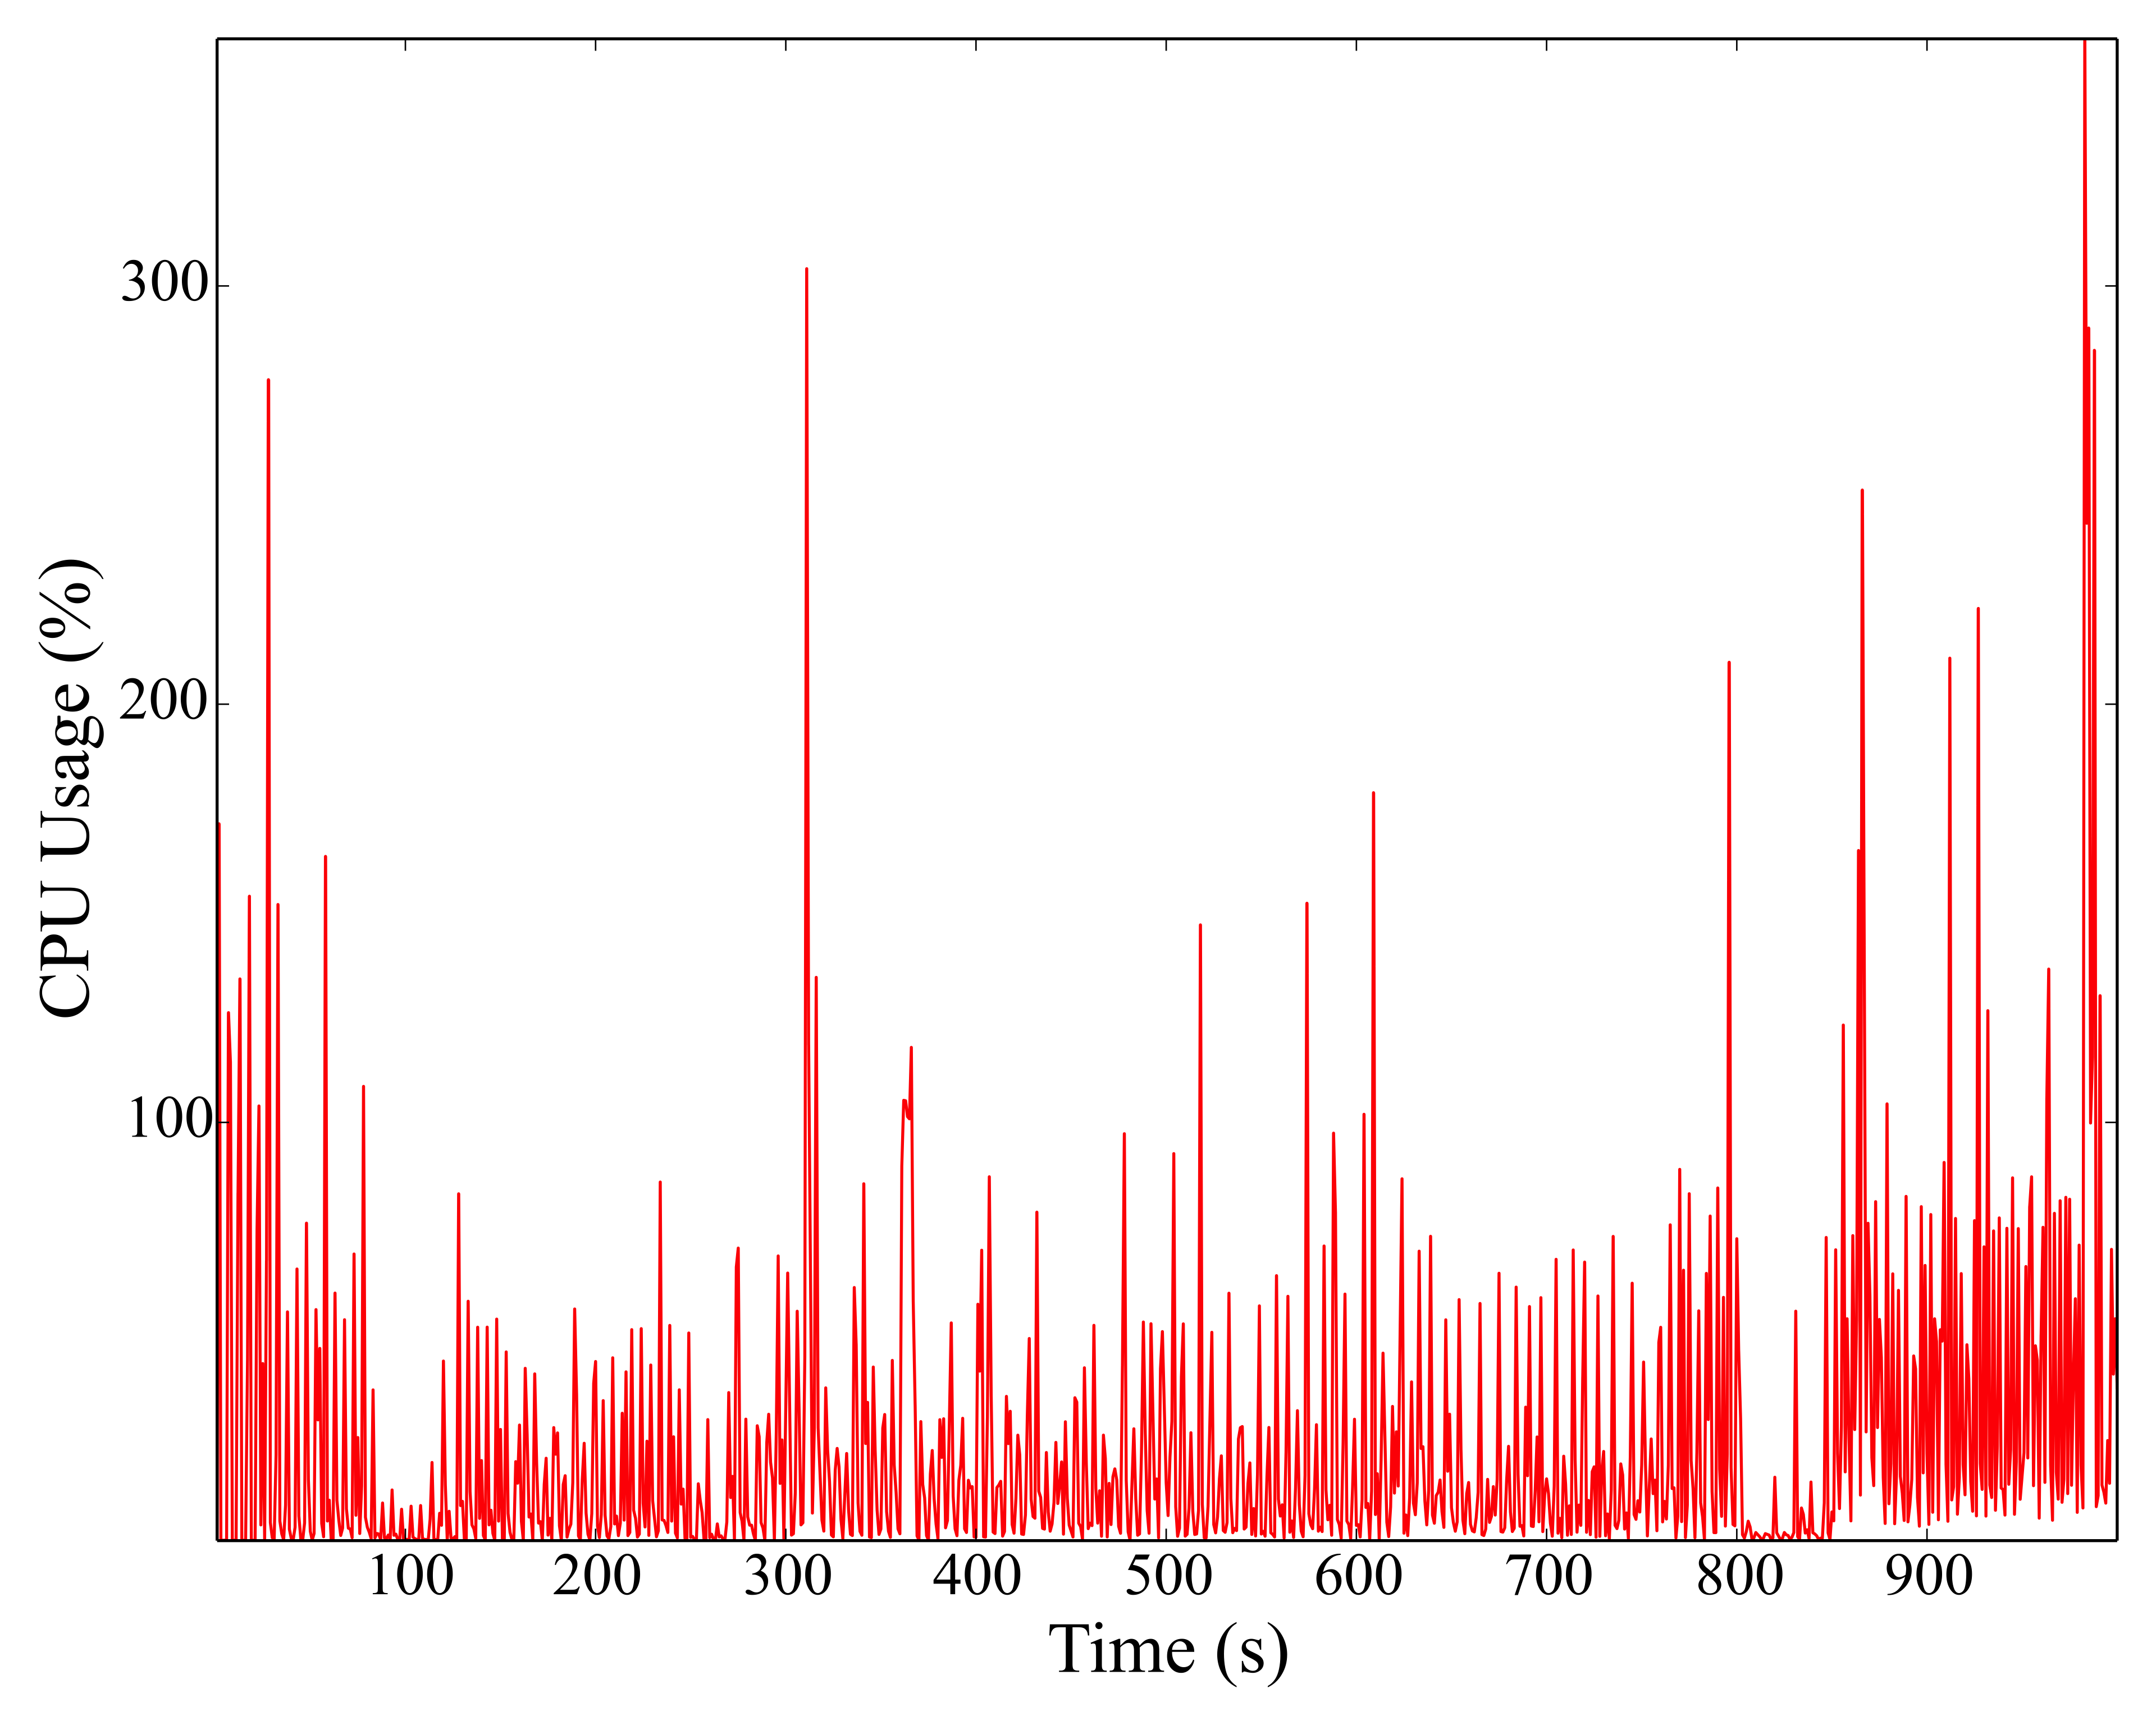
\includegraphics[width=0.45\textwidth]{pic/webmagic40ms100.png}
  }
  
  % \\
  \subcaptionbox{\footnotesize {100ms延迟场景}}{
    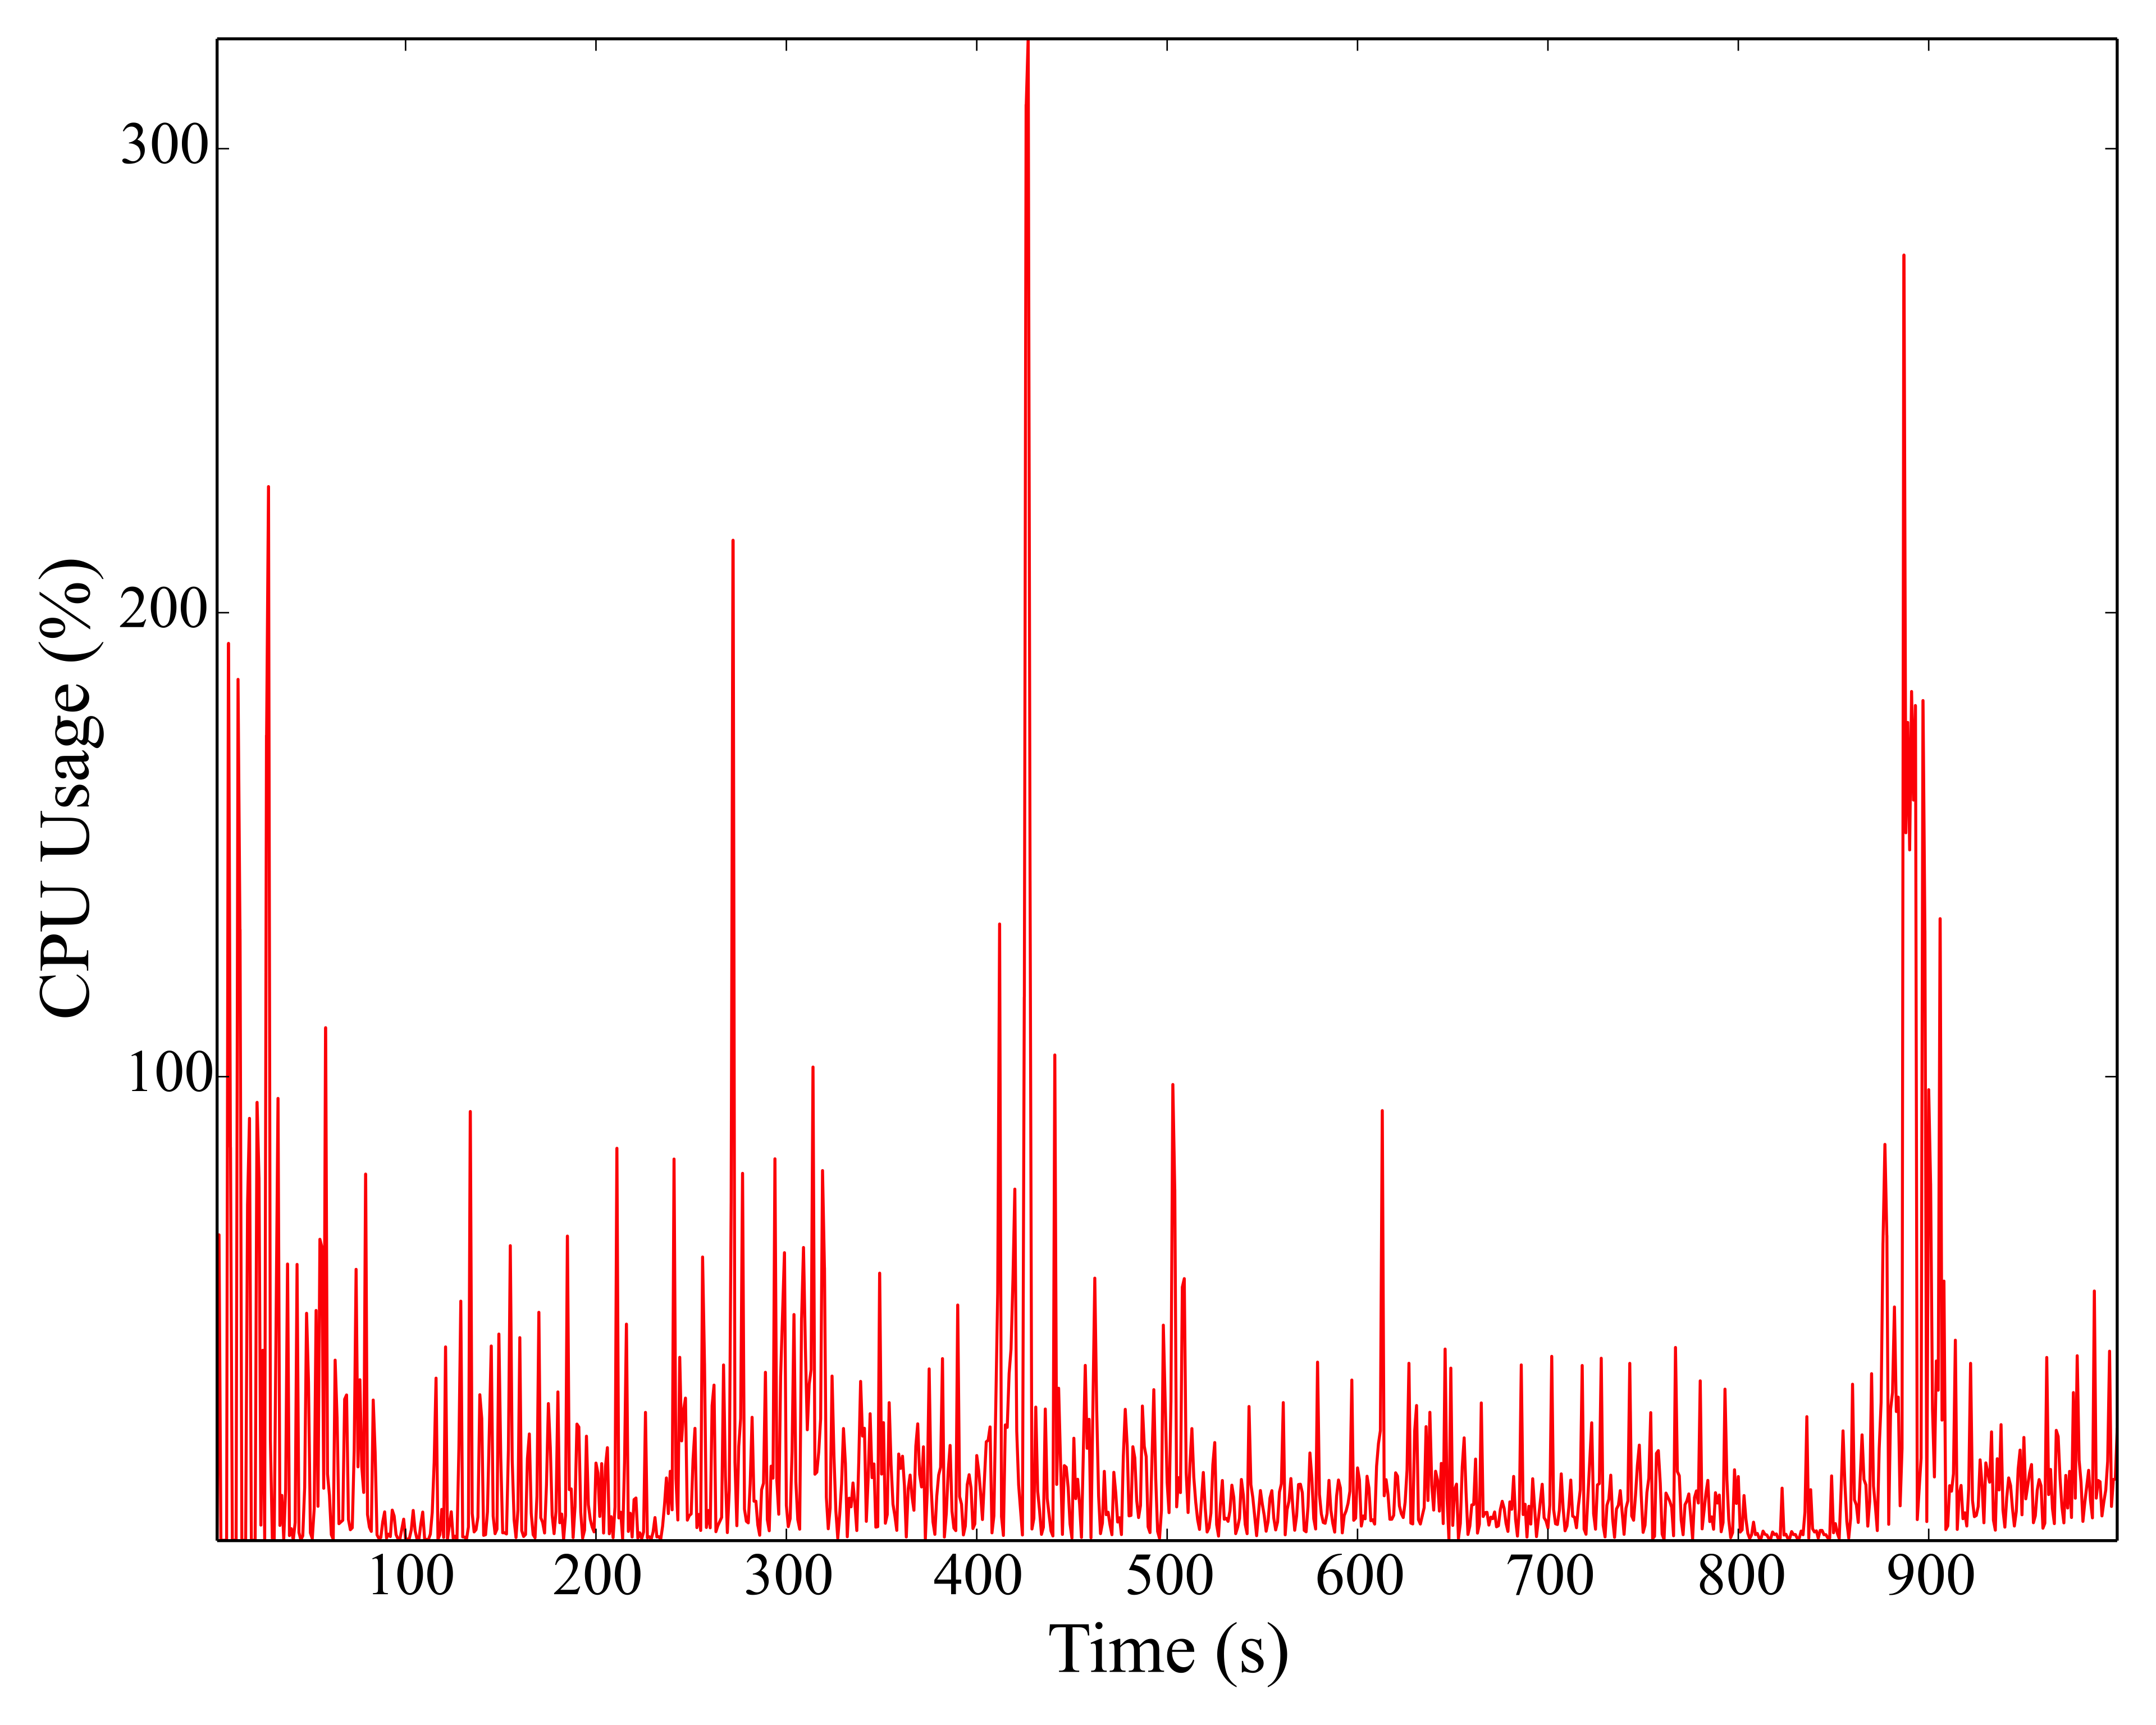
\includegraphics[width=0.45\textwidth]{pic/webmagic100ms100.png}
  }
  \hfill
  \subcaptionbox{\footnotesize {200ms延迟场景}}{
    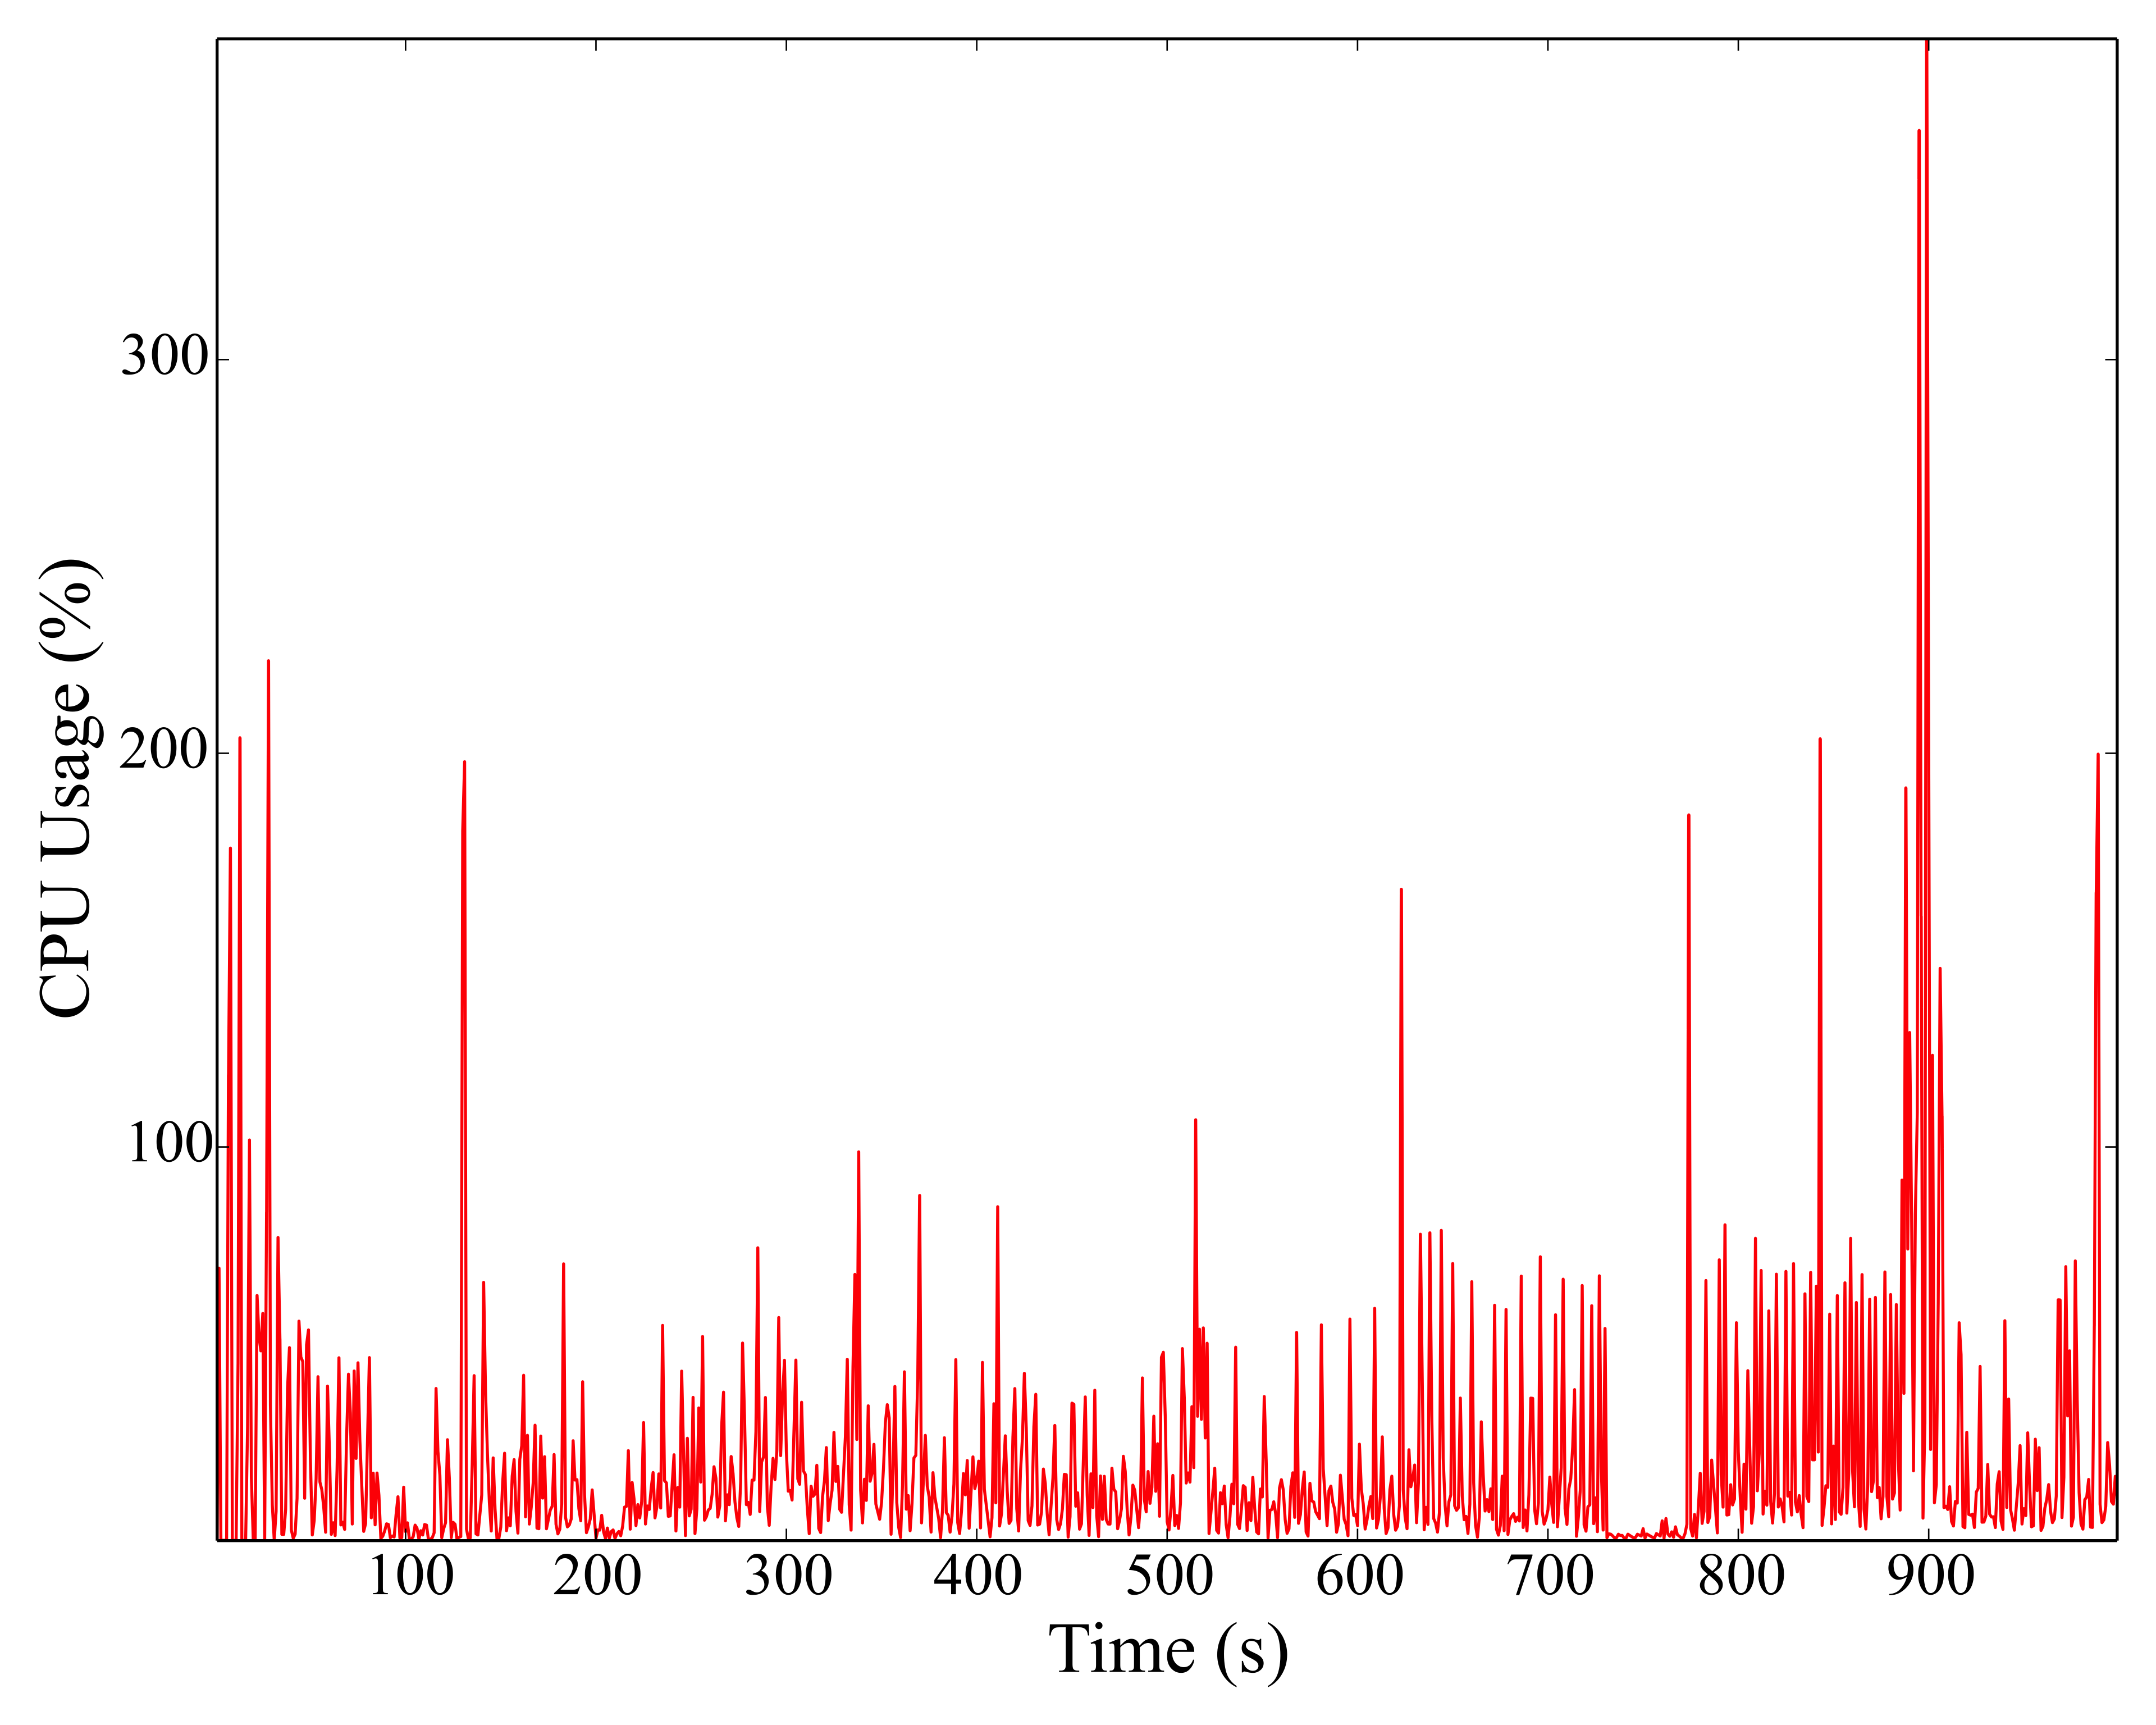
\includegraphics[width=0.45\textwidth]{pic/webmagic200ms100.png}
  }
\caption{Webmagic100并发度不同时延下的CPU利用率}\label{40ms}
\end{figure}

为了模拟真实网站响应时延,实验分别设置40ms、100ms、200ms发包时延。如图\ref{40ms} 所示,这是Webmagic爬虫在100并发度下40ms,100ms,200ms延迟设定时的CPU使用率情况。我们发现不同延迟场景下的CPU使用情况并无太大的明显差异。

Spidereact爬虫CPU利用率如图\ref{fig:spidereact} 所示, 在不同时延设置下,Spidereact爬虫的CPU资源使用率始终能够维持在100\%以上,CPU利用率存在一定的波动,但波动范围并没有Webmaigc爬虫表现得那么剧烈。这是由于Spidereact为了能够减少线程切换的开销,异步线程池的并发度默认设置成了CPU核数的10倍,
同时由于Spidereact的异步非阻塞编程模型,线程池的增加,并发度的加大并不会对爬虫的性能造成有利的影响,真正影响爬虫效率的关键在于CPU运行非阻塞的页面解析代码的效率。所以
实验按照了Spideract的默认并发度来进行对比。和Webmagic爬虫相比,可以发现Spidereact爬虫的CPU利用率明显高于Webmagic爬虫的CPU利用率。
\begin{figure}[!htbp]
\centering
\subcaptionbox{\footnotesize {0时延}}{
    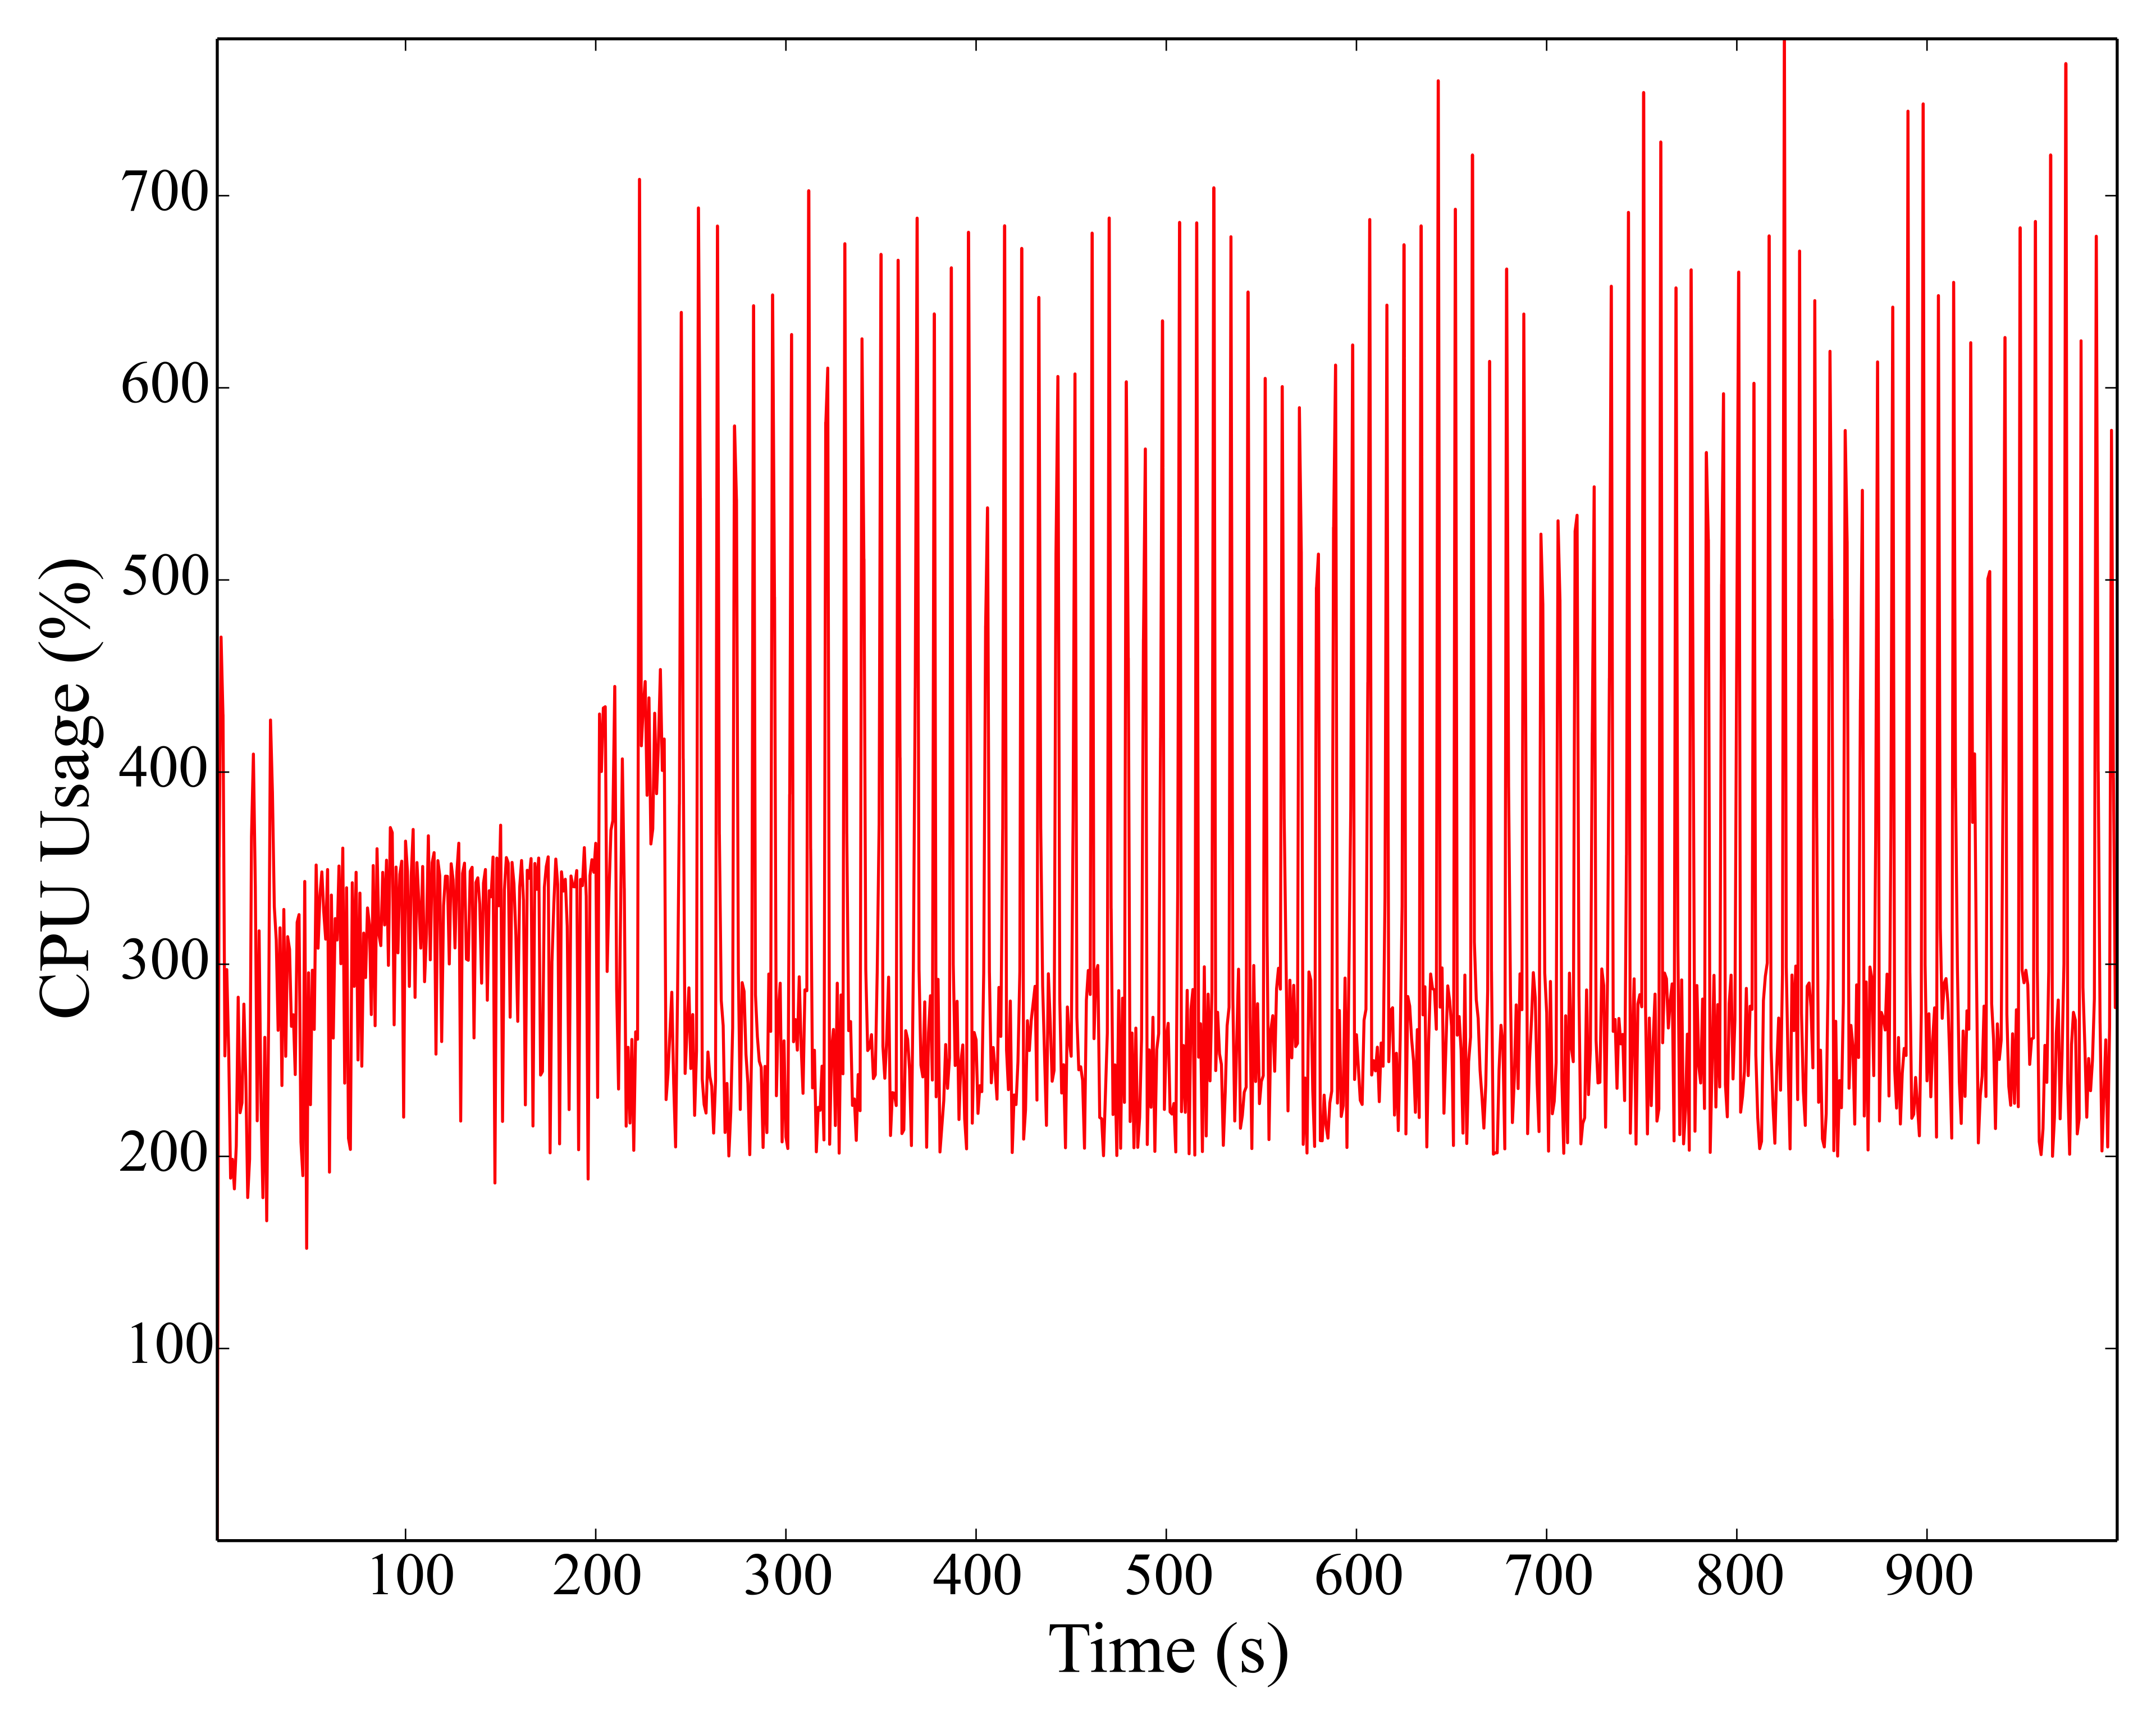
\includegraphics[width=0.45\textwidth]{pic/spidereact0ms.png}
  }
  \hfill
  \subcaptionbox{\footnotesize {40ms时延}}{
    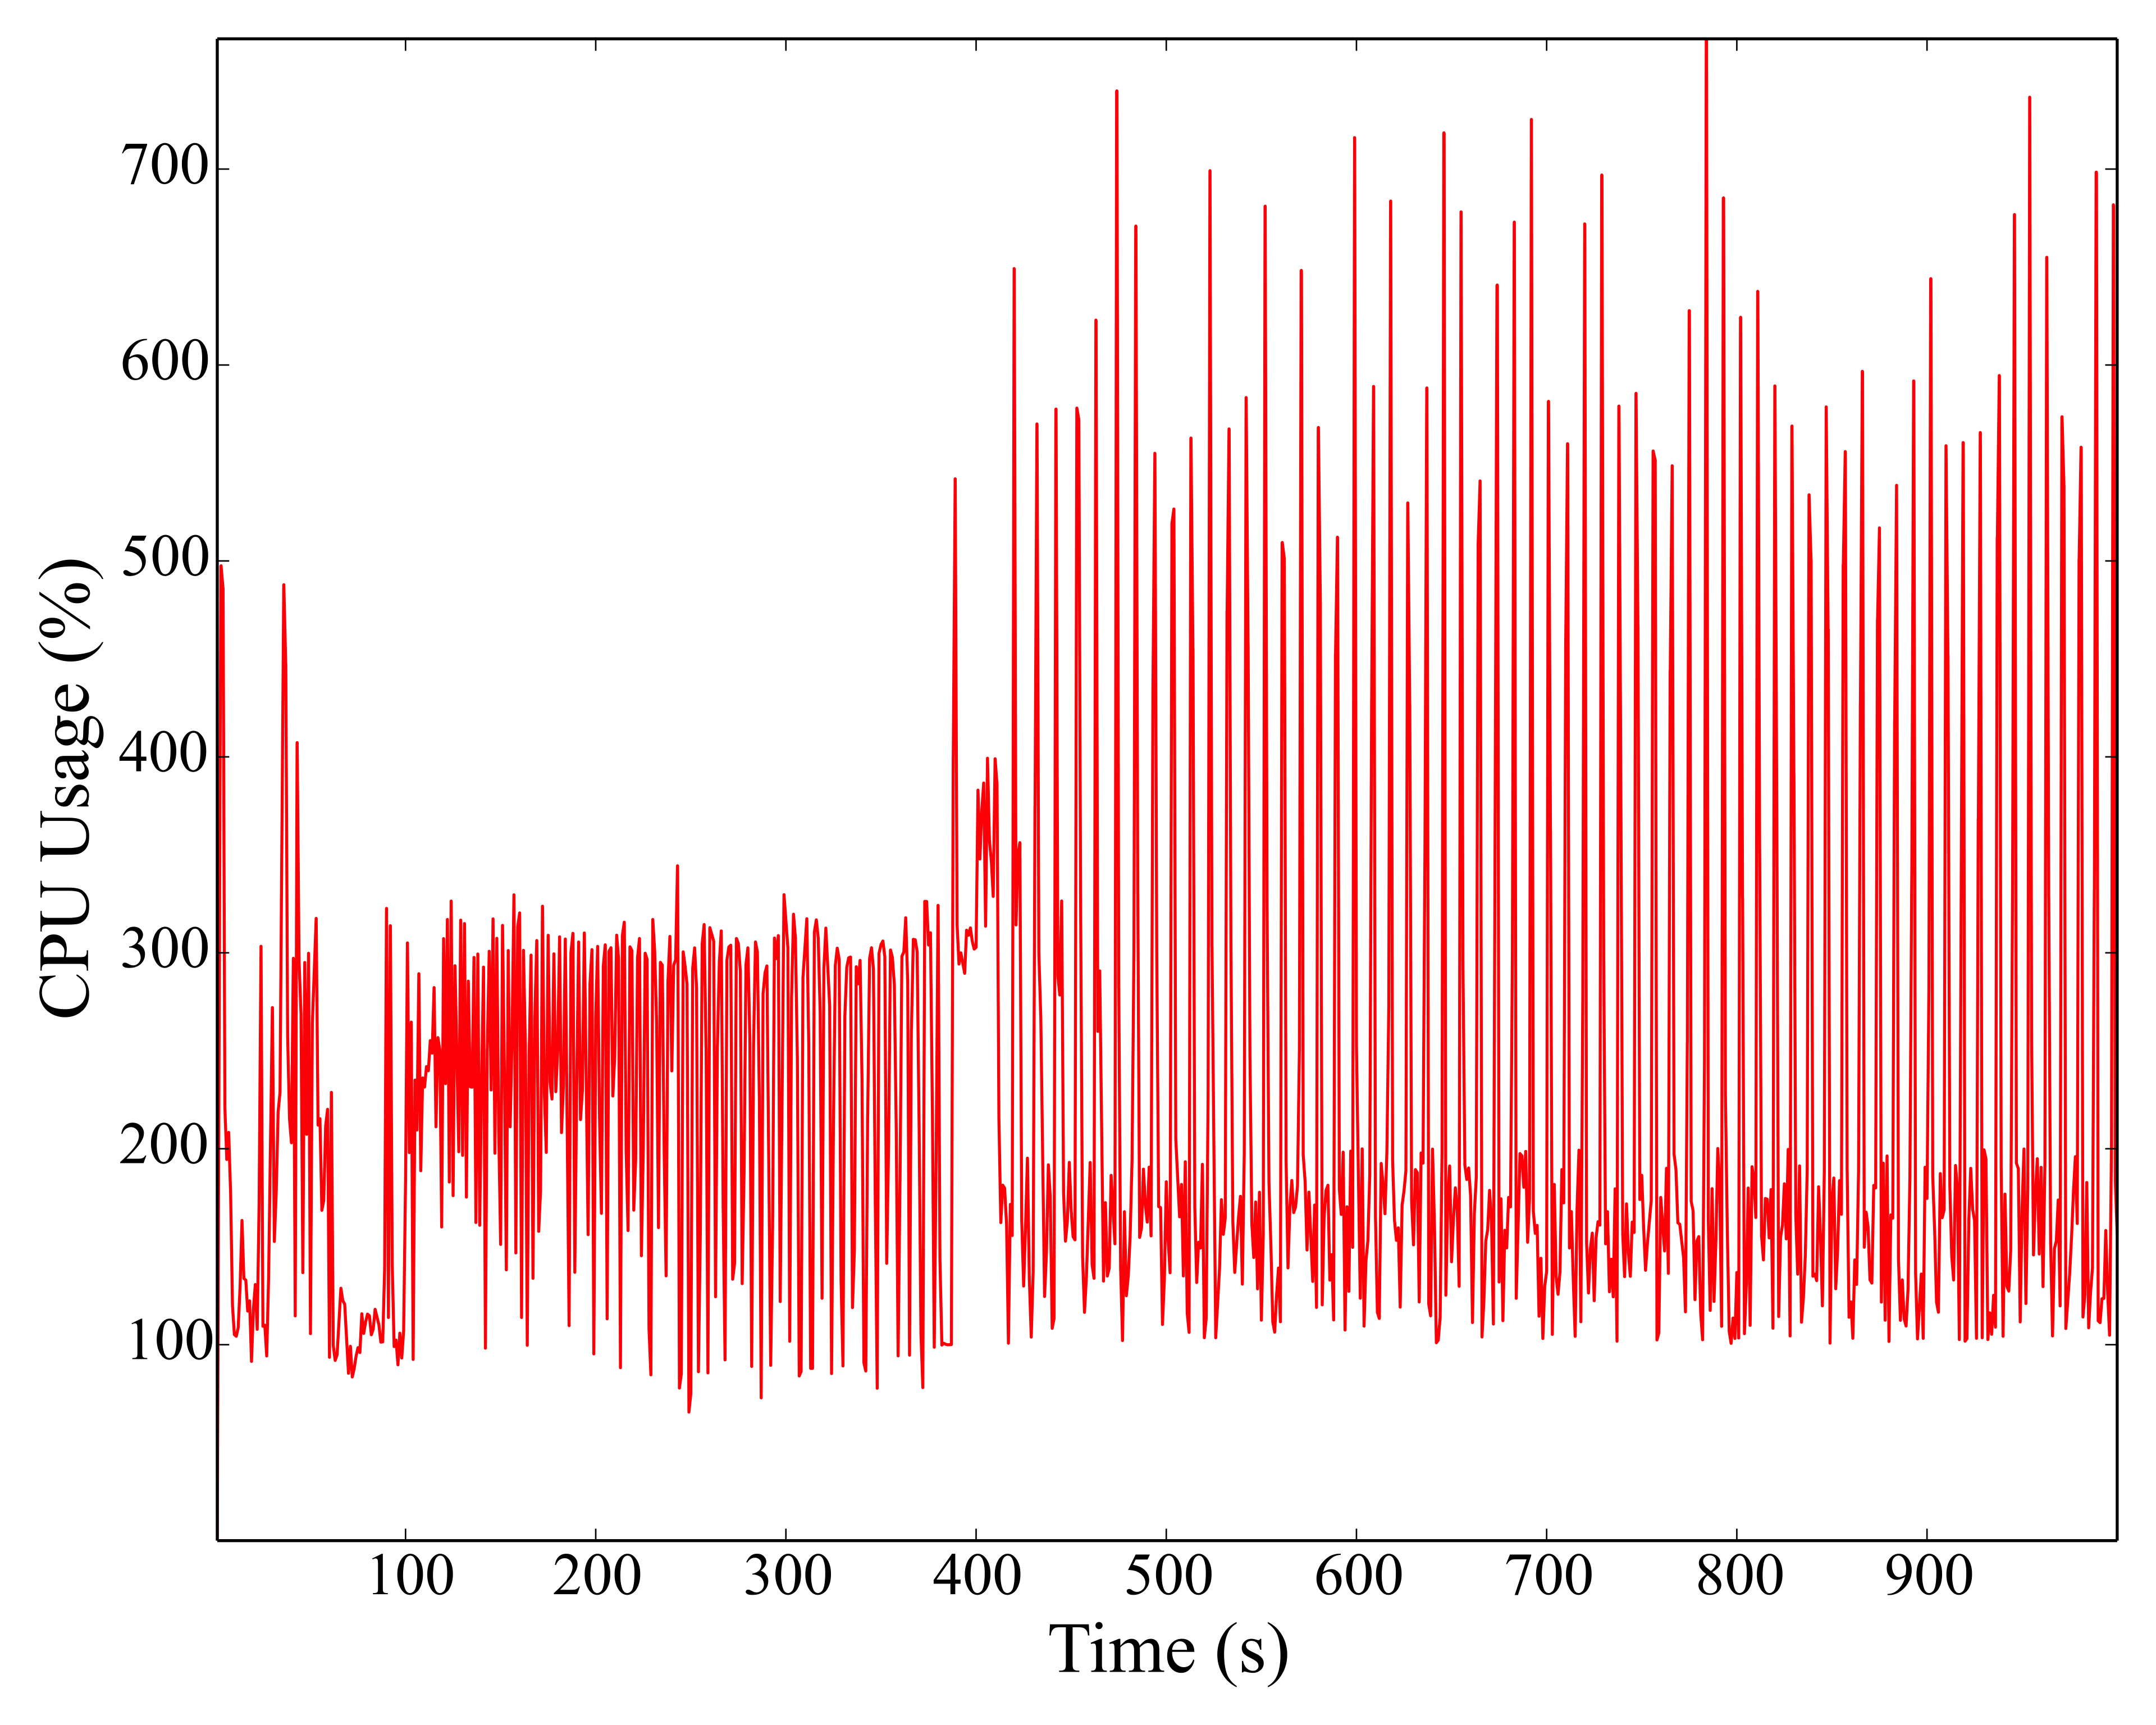
\includegraphics[width=0.45\textwidth]{pic/spidereact40ms.png}
  }
  \\
  \subcaptionbox{\footnotesize {100ms时延}}{
    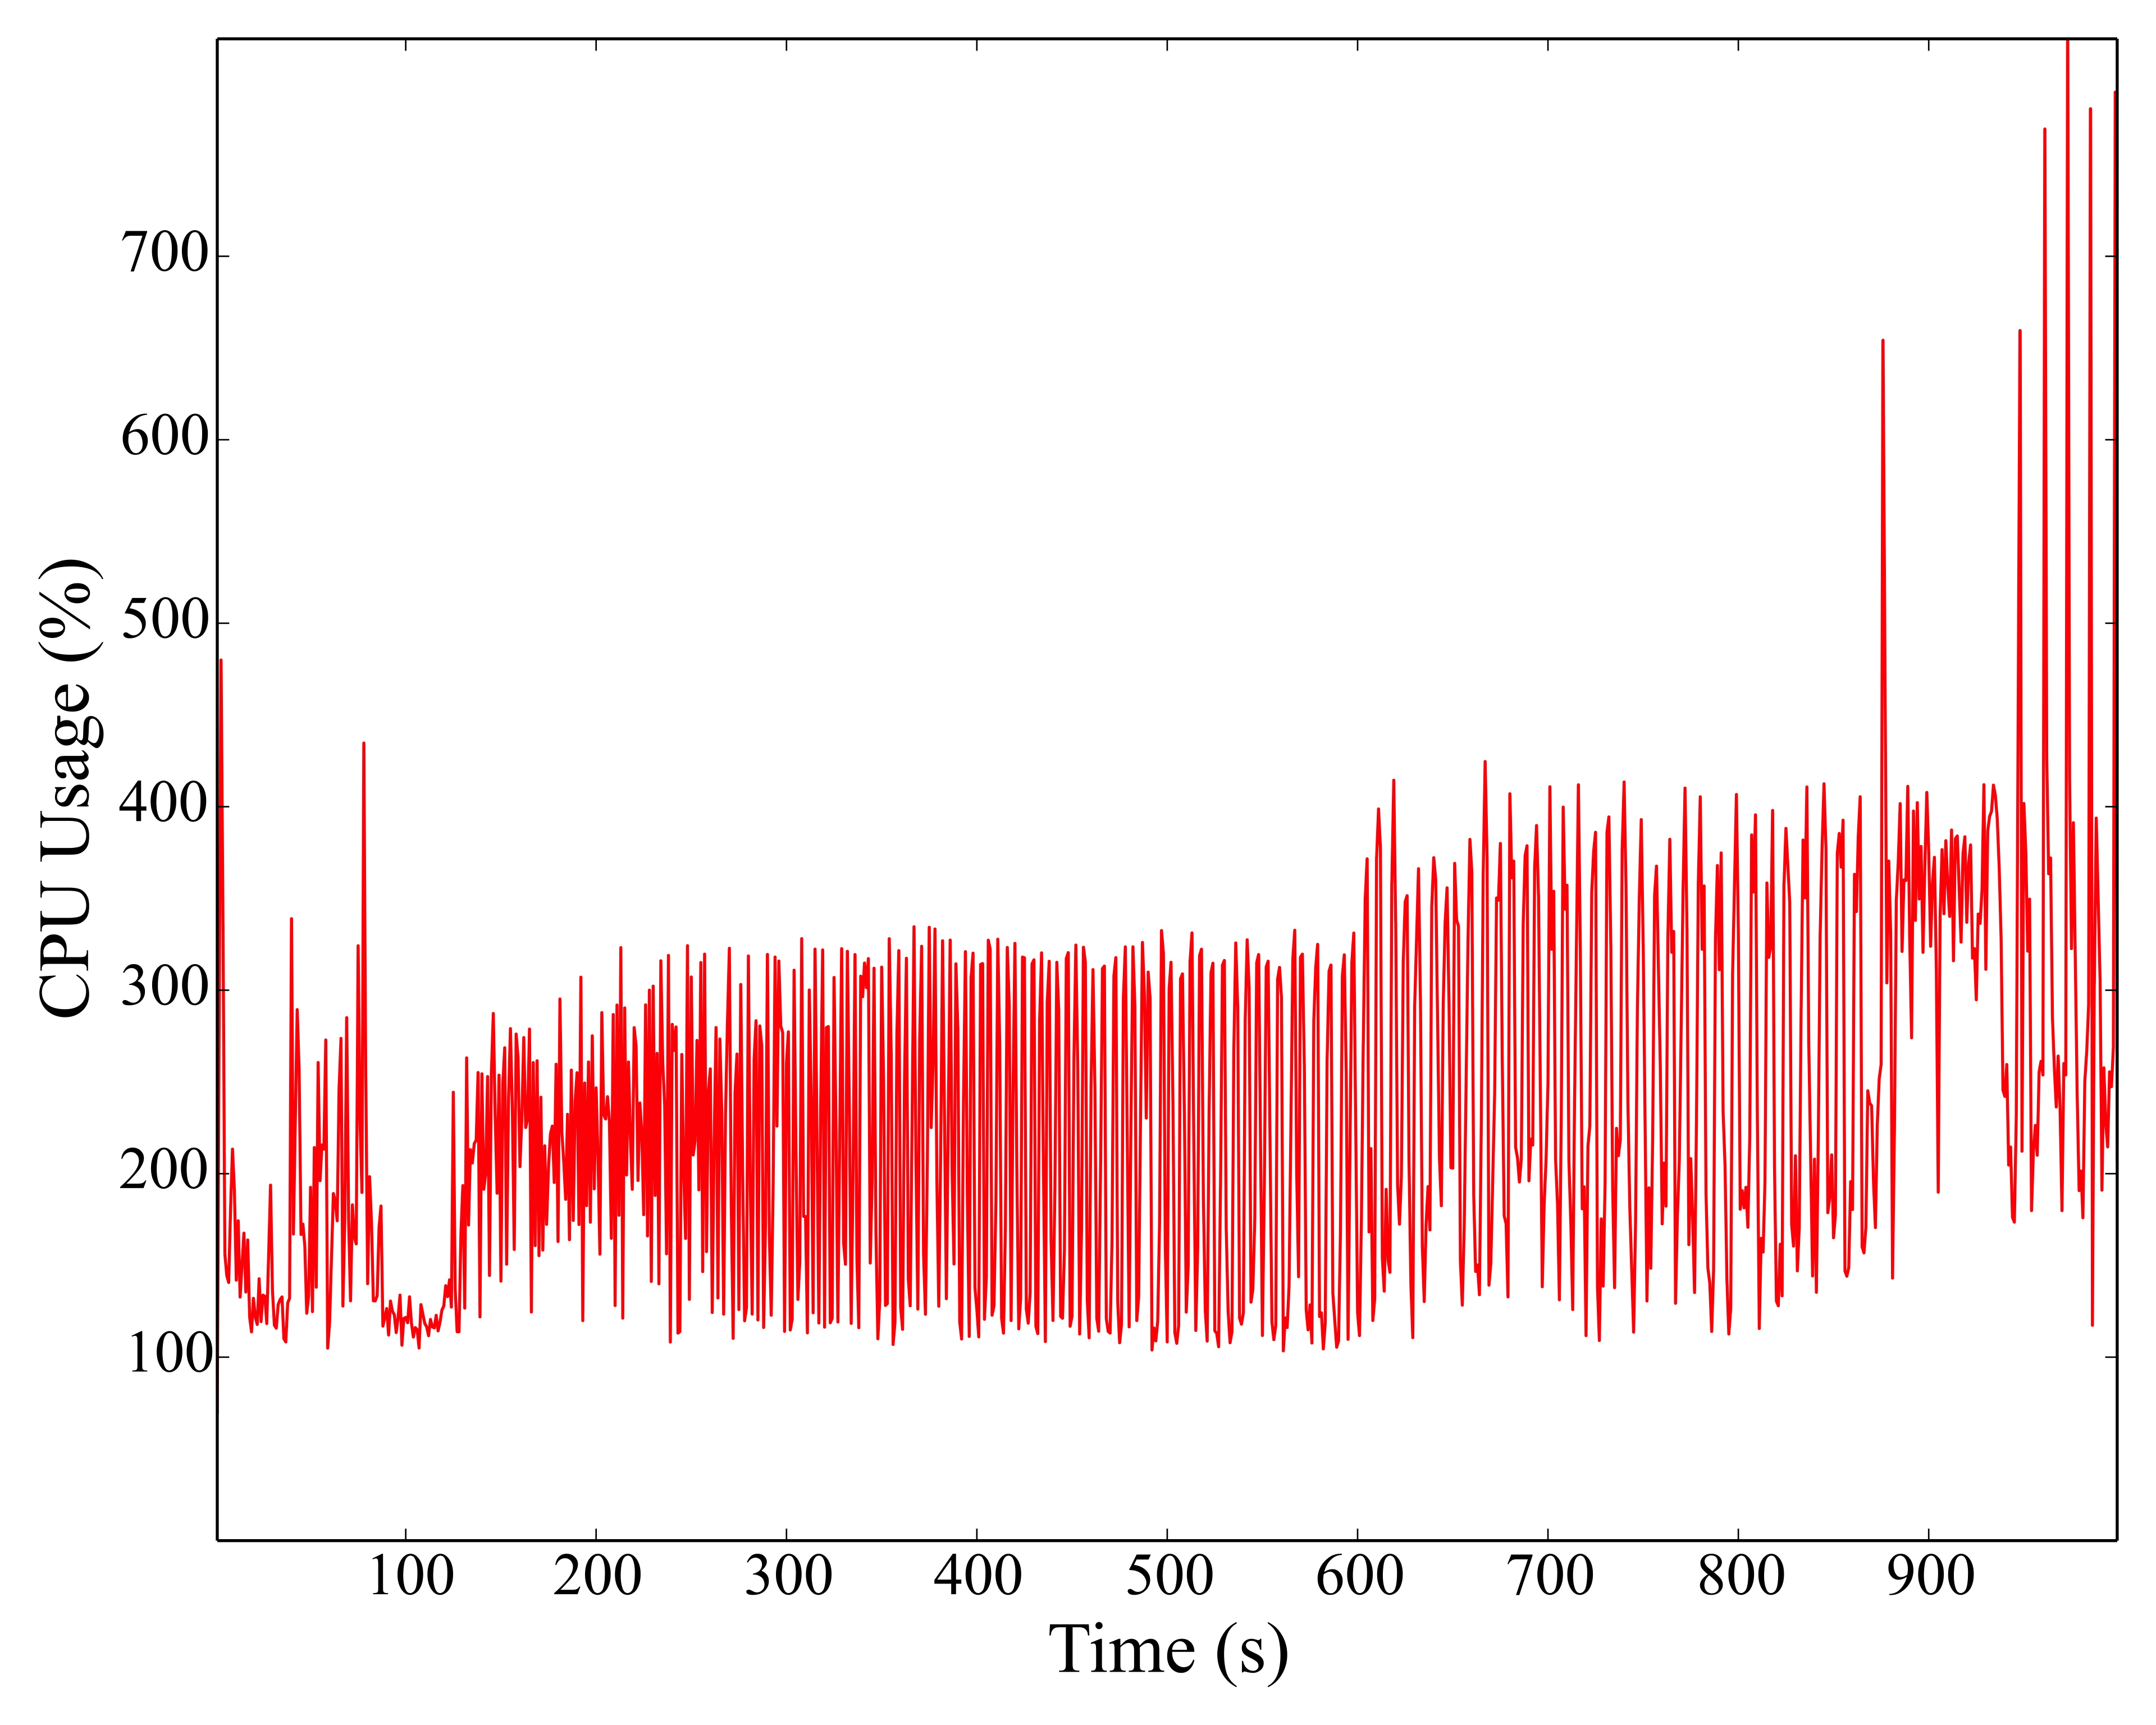
\includegraphics[width=0.45\textwidth]{pic/spidereact100ms.png}
  }
  \hfill
  \subcaptionbox{\footnotesize {200ms时延}}{
    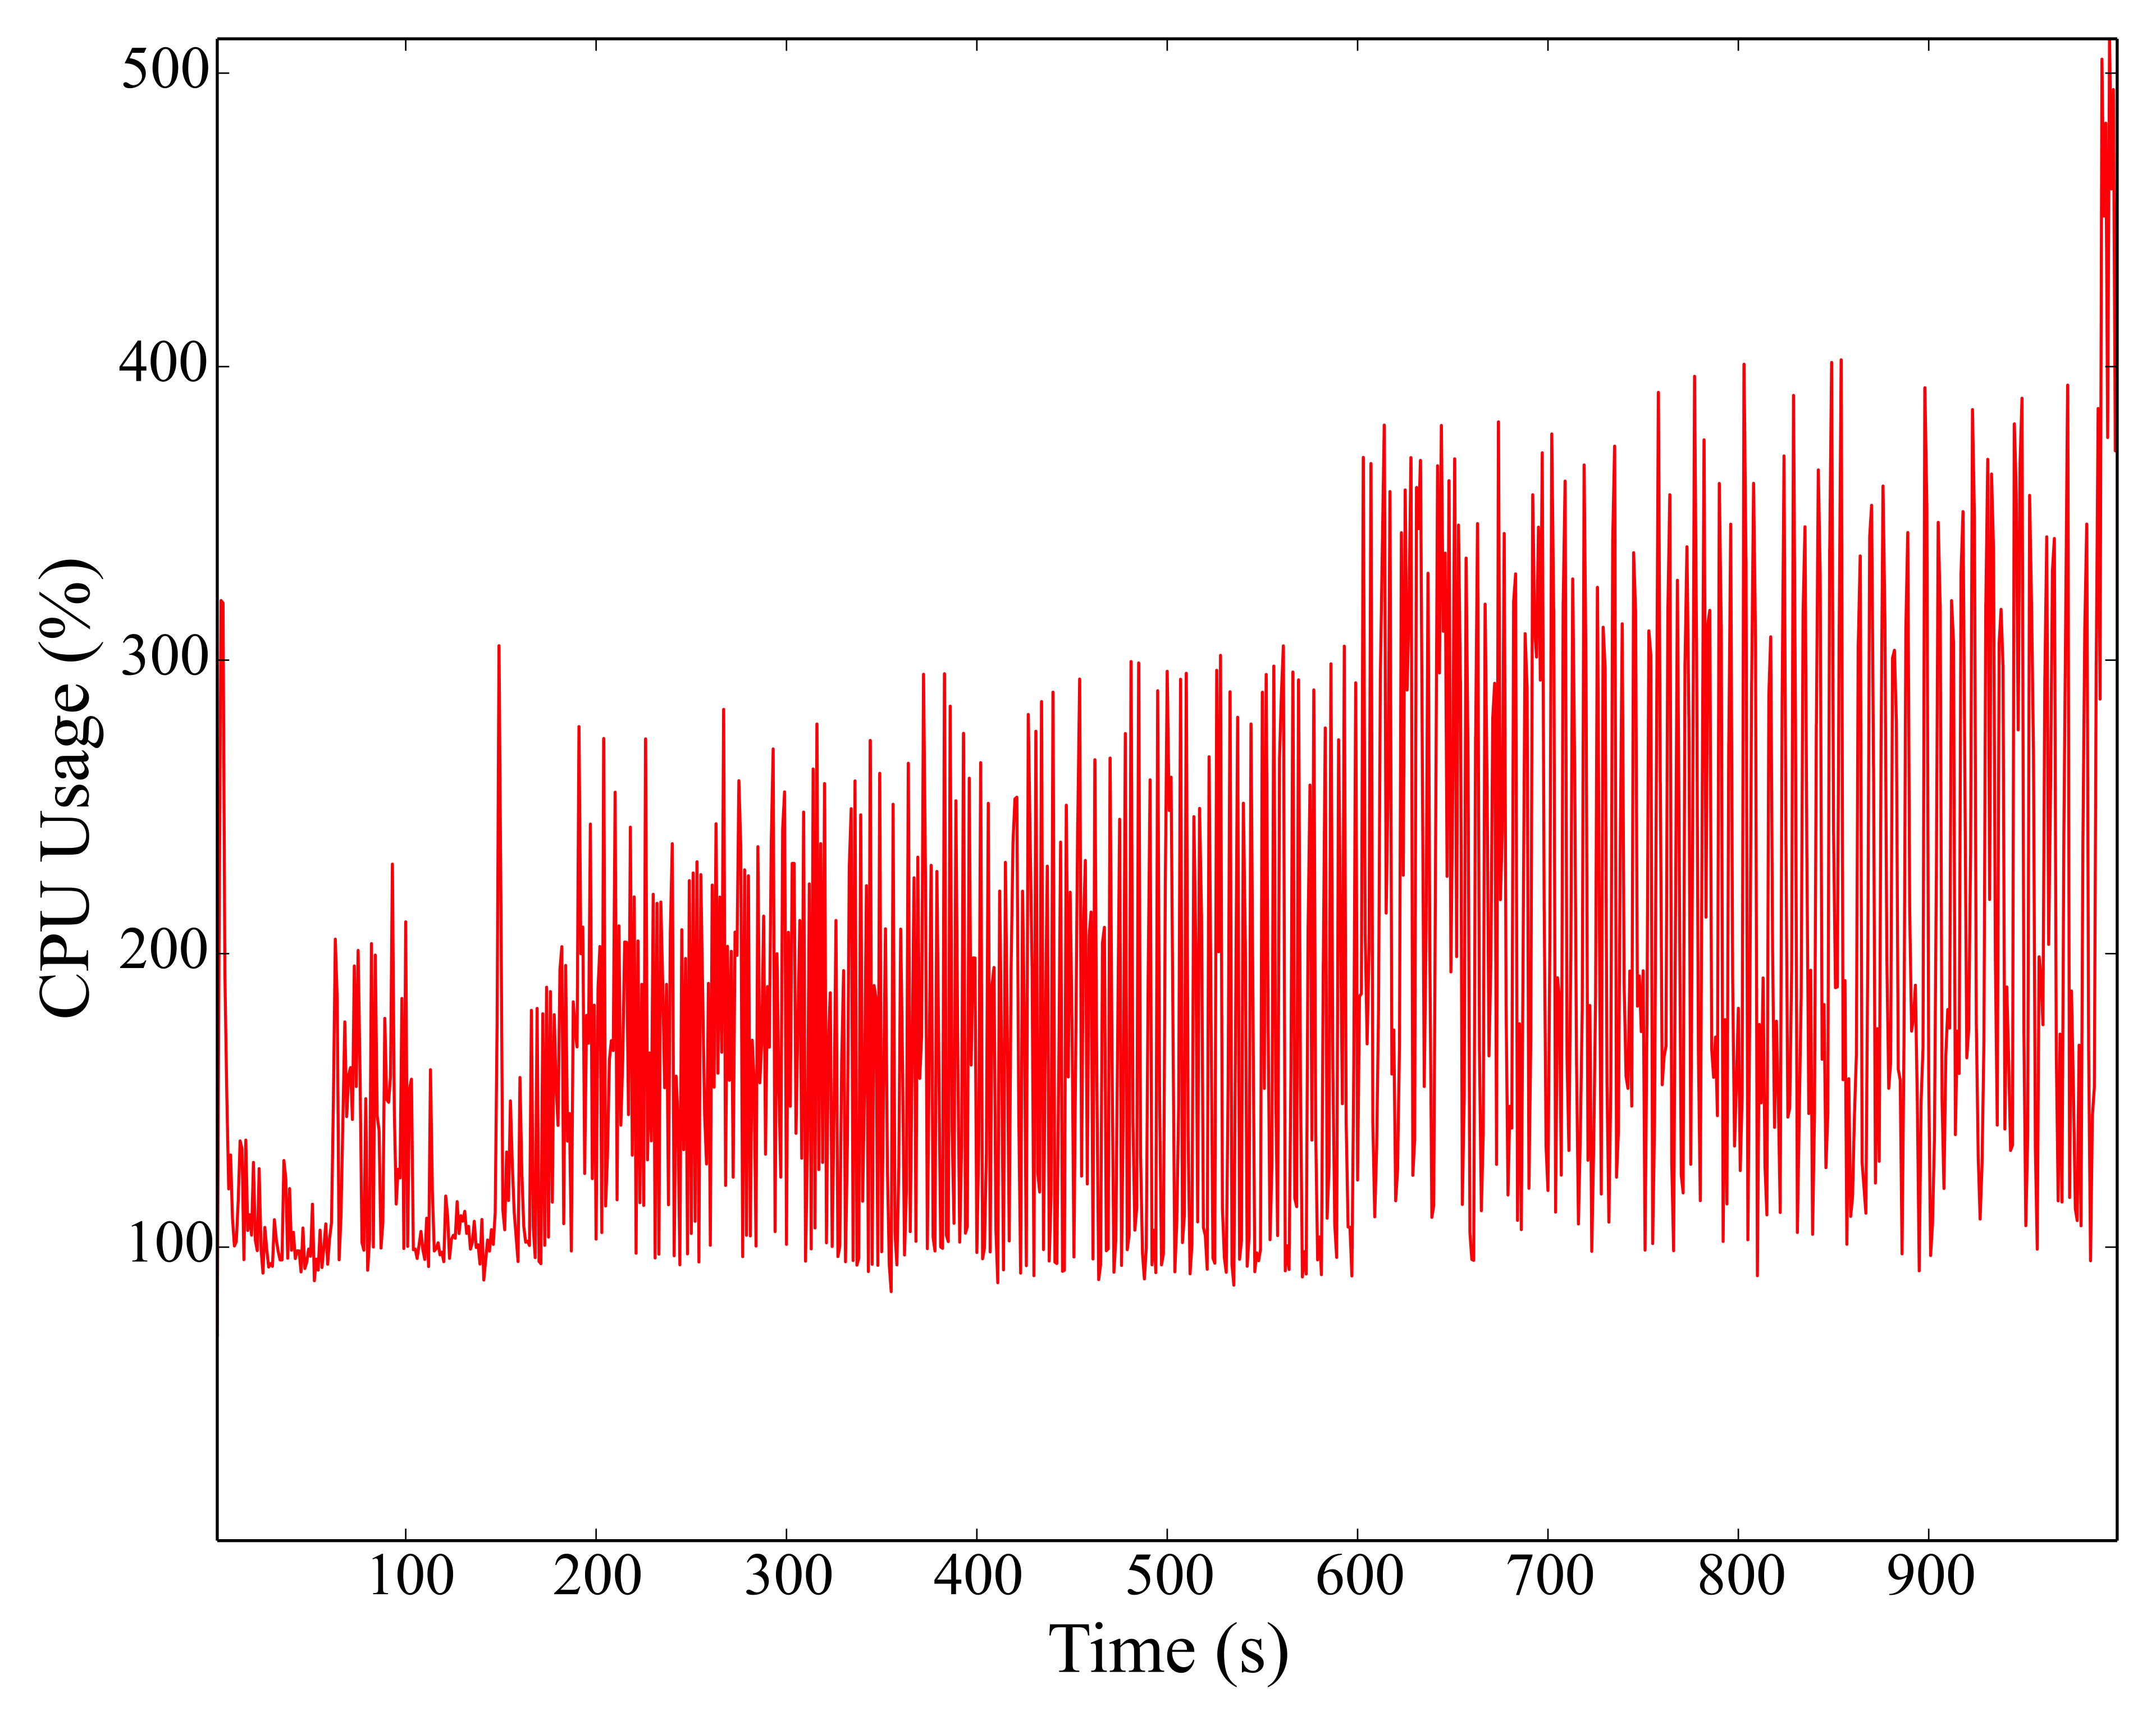
\includegraphics[width=0.45\textwidth]{pic/spidereact200ms.png}
  }
\caption{Spidereact 40并发下不同时延下CPU使用情况}\label{fig:spidereact}
\end{figure}


\subsection{吞吐量对比}
为了测试了Spidereact爬虫的吞吐量,实验将Spidereact实现的爬虫和Webmaigc实现的爬虫进行了吞吐量之间的比较。
首先,在并没有设置任何时延的情况下,实验先比较了Webmagic在不同并发下的吞吐量情况。如图\ref{webmagic-con} 所示,
可以发现,当并发度较小的时候,吞吐量与并发度之间存在着线性关系,并发度提高,吞吐量也随之线性增长。但是当并发度
超过400之后,爬虫的吞吐量就没有随之并发度的提高而增长,而是在80上下起伏。这种情况也符合我们的预期,因为对于
多线程模型Webmagic爬虫来说,由于它从下载、解析、处理整个同步流程都是在同一个线程中进行的,整个过程都是线程并发
执行的,其加速比是固定的,所以并发度较小的时候,随着线程数的增多,吞吐量呈现线性增长。但当并发度上升到一定程度之后,
导致CPU并发线程过多,线程上下文切换频繁,内存消耗增加,从而使得吞吐量可能还会下降。从图\ref{webmagic-con} 中也可以
看出并发度在500至1000之间变化时,吞吐量有时反而还下降了。抛去偶然因素的影响,吞吐量稳定在一个数值左右。
后续与Spidereact的对比实验中,实验分别采样了Webmagic在100、300、600、1000并发下的吞吐量数值。
% 然而,前面的网站压测实验数据表明,网站是可以承受1000的并发度的。

\begin{figure}
\centering
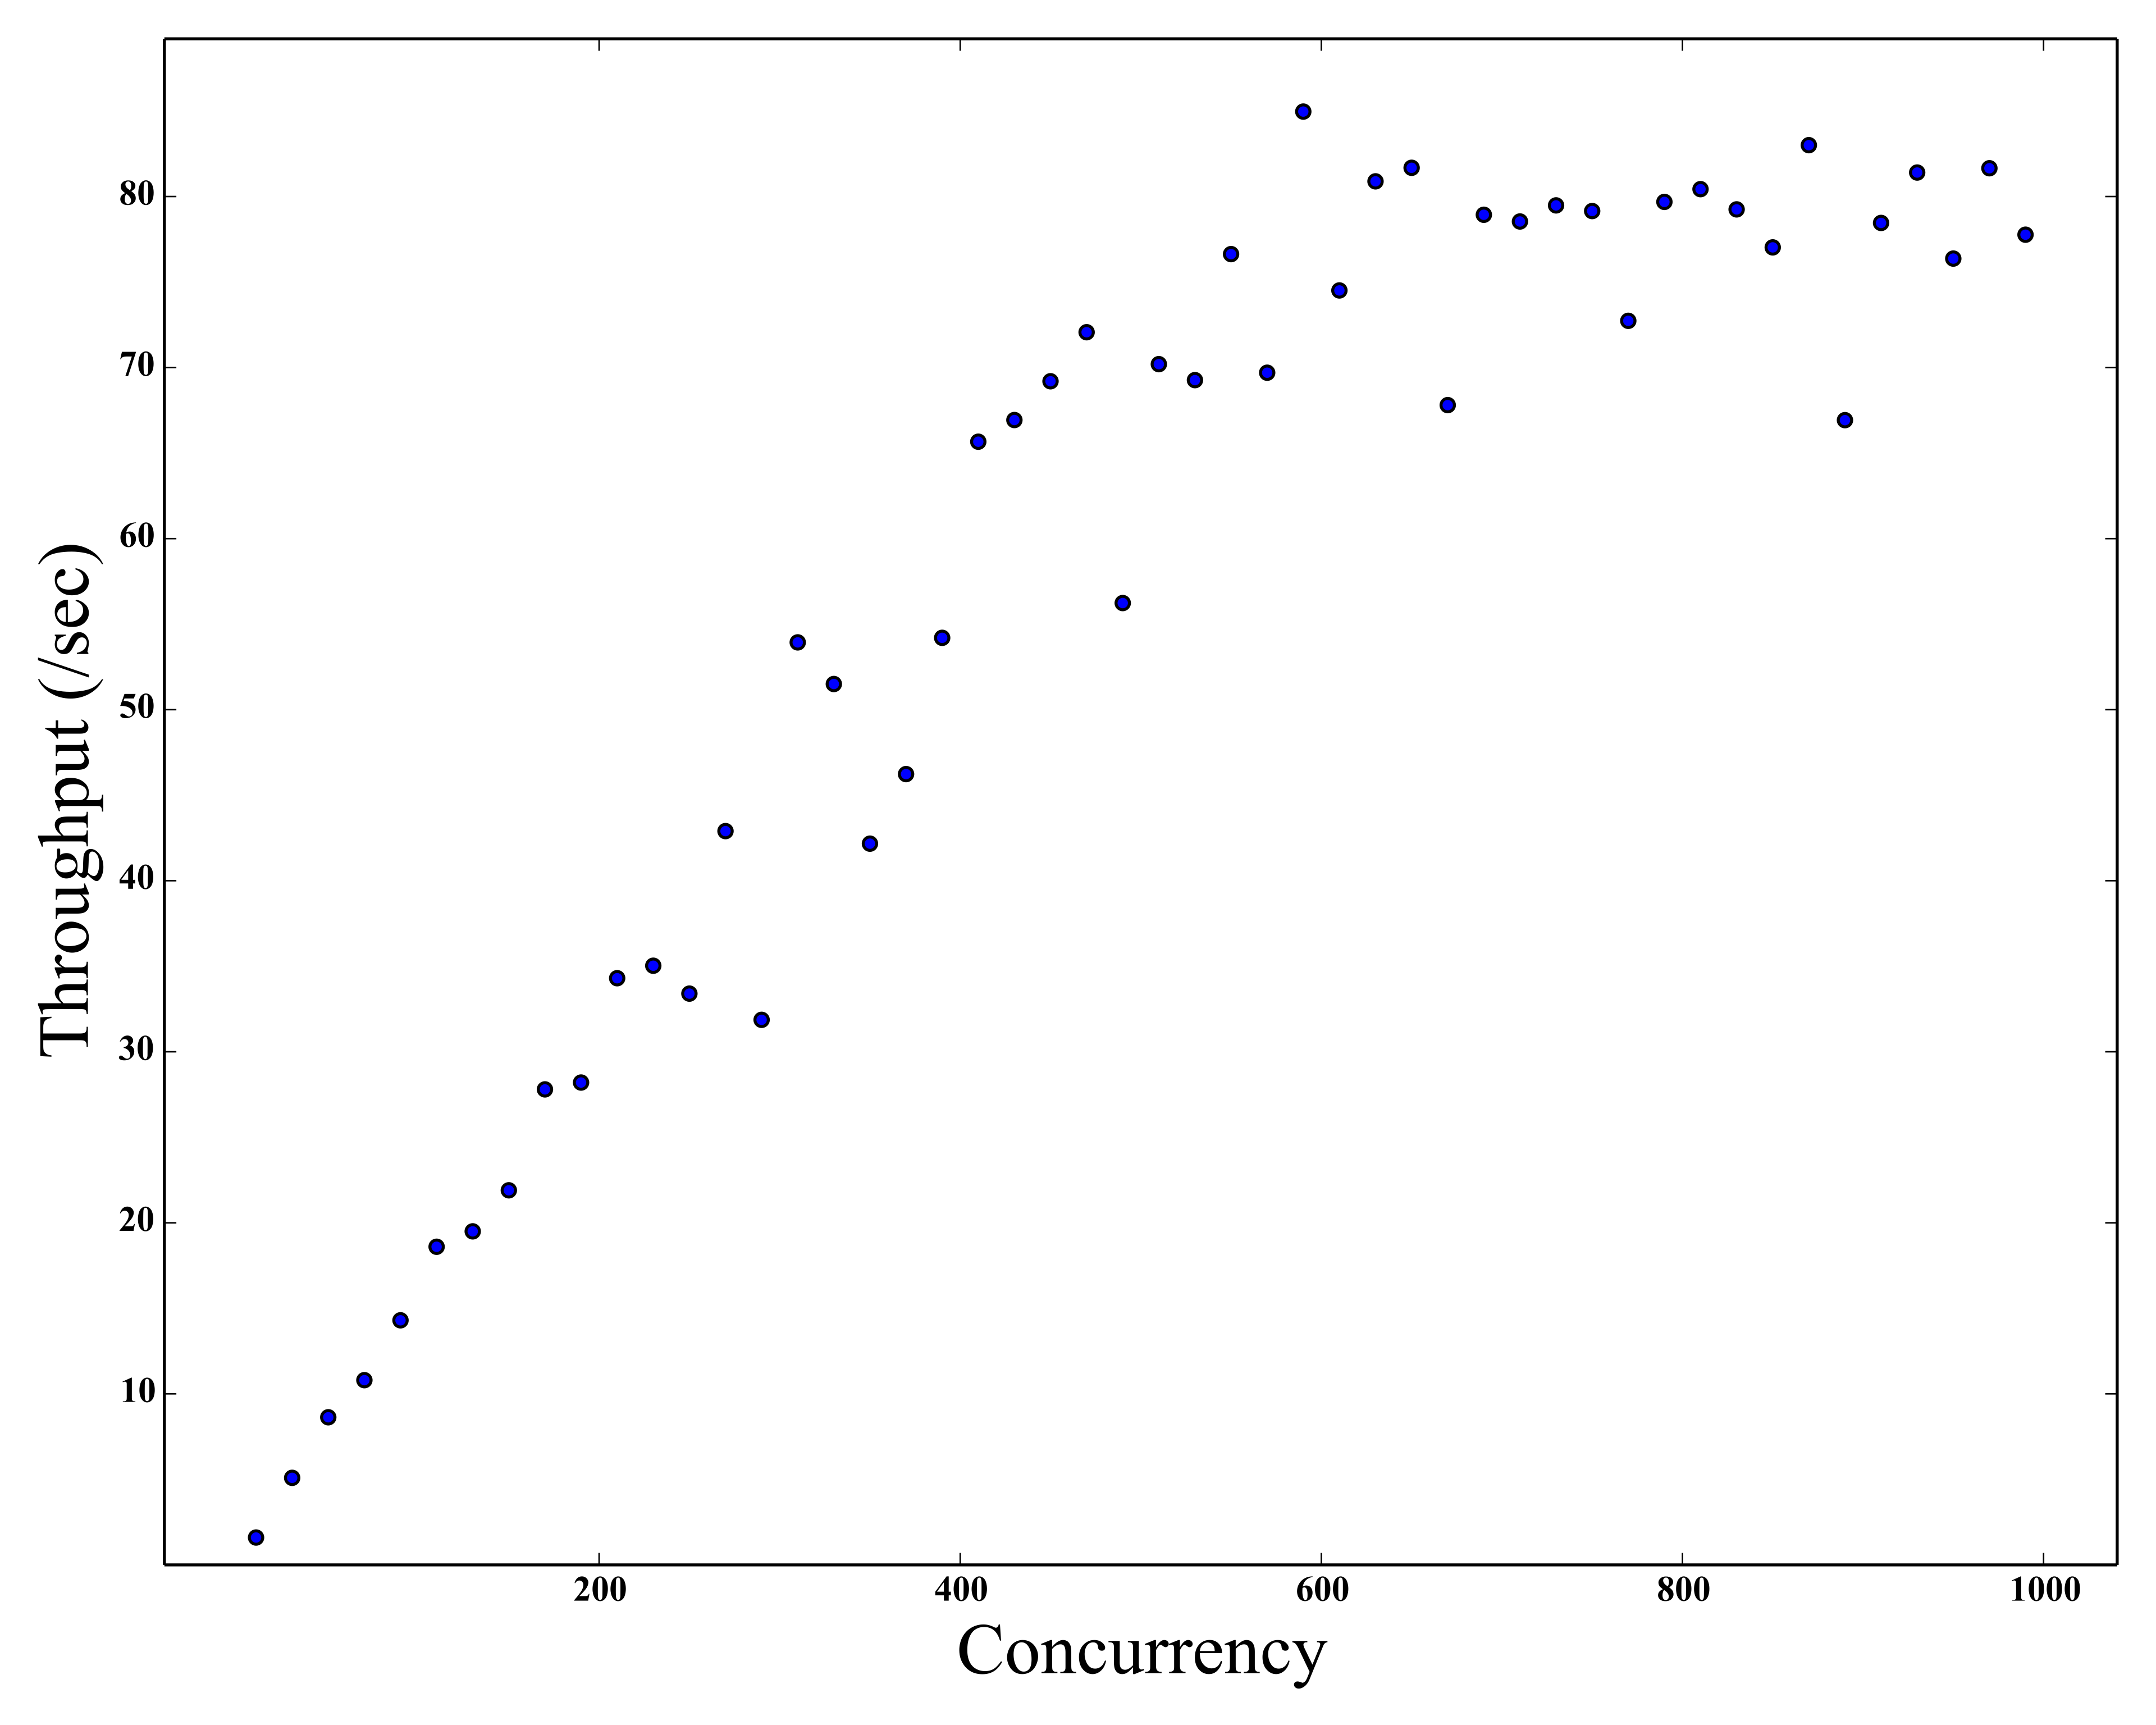
\includegraphics[width=0.8\textwidth]{pic/concurrent.png}

\caption{Webmagic不同并发下吞吐量}\label{webmagic-con}
\end{figure}


正如前文所提到的,Spidereact是基于Project Reactor开发的响应式爬虫框架,其并发度默认为系统的CPU核数的10倍,在本次实验中,Spidereact的并发度看作
是40。通过表\ref{table:throughputAll} 将Webmagic各个并发度的吞吐量和Spidereact的对比,我们发现,在Spidereact在吞吐量方面要优于Webmagic,Spidereact可以
用更少的资源,达到更高的吞吐量。

\begin{table}
\centering
\begin{tabular}{|c|c|c|c|c|}
\hline
实验并发度& 延迟设置 & 爬取总量 & 时间(ms) & 吞吐量(/sec) \\
Webmagic-100并发 & 0ms  & 13705 & 1000000 & 13.7 \\
Webmagic-100并发 & 40ms & 13060 & 1000000 & 13.06 \\
Webmagic-100并发 & 100ms & 12932 & 1000000 & 12.9 \\
Webmagic-100并发 & 200ms & 12668 & 1000000 & 12.7 \\
Webmaigc-300并发 & 0ms  & 36413 & 1000000 & 36.4 \\
Webmagic-300并发 & 40ms & 37336 & 1000000 & 37.3 \\
Webmagic-300并发 & 100ms & 36854 & 1000000 & 36.8 \\
Webmagic-300并发 & 200ms & 35993 & 1000000 & 36.0 \\
Webmagic-600并发 & 0ms  & 89482 & 1000000 & 89.5 \\
Webmagic-600并发 & 40ms & 75322 & 1000000 & 75.3 \\
Webmagic-600并发 & 100ms & 72038 & 1000000 & 72.0 \\
Webmagic-600并发 & 200ms & 70142 & 1000000 & 70.1 \\
Webmagic-1000并发 & 0ms  & 85839 & 1000000 & 85.8 \\
Webmagic-1000并发 & 40ms & 70026 & 1000000 & 70.0 \\
Webmagic-1000并发 & 100ms & 67928 & 1000000 & 67.9 \\
Webmagic-1000并发 & 200ms & 67402 & 1000000 & 67.4 \\
Spidereact & 0ms  & 202530  & 1000000 & 202.5 \\
Spidereact & 40ms & 176721 & 1000000 & 176.7 \\
Spidereact & 100ms & 164236 & 1000000 & 164.2 \\
Spidereact & 200ms & 158825 & 1000000 & 158.8 \\
\hline
\end{tabular}
\caption{不同延迟不同并发下吞吐量对比}\label{table:throughputAll}
\end{table}
% \begin{table}
% \centering
% \begin{tabular}{|c|c|c|c|}
% \hline
% 实验对象 & 爬取总量 & 时间(ms) & 吞吐量(/sec) \\
% \hline
% Webmagic-100并发 & 2041 & 149243 & 13.7 \\
% Webmaigc-300并发 & 5574 & 152512 &36.4 \\
% Webmagic-600并发 & 10472 & 116630 & 89.5 \\
% Webmagic-1000并发 & 11327 & 132741 & 85.8 \\
% Spidereact & 20663  & 102649 & 202.5 \\
% \hline
% \end{tabular}
% \caption{吞吐量对比}\label{table:throughput}
% \end{table}

% \subsection{模拟延迟}
% 上面提到的并发实验是针对一个模拟的静态网站的爬取,和真实网站不同的是,爬虫的请求发送到网站后,网站能够很快的响应,因为没有
% 额外的处理流程,只是将存储的静态网页返回给了爬虫。为了更进一步模拟真实网站爬取,我们通过Linux下的一个流量控制工具tc(traffic control)来控制网站端的发包操作,
% tc控制直接对物理网卡生效,我们将物理网卡的发包时延设置40ms、100ms、200ms来延迟发送,并设置延迟时间有上下10ms的波动,
% 来模拟真实网络环境中的请求时延迟。

各个延迟场景下吞吐量对比如表\ref{table:throughputAll} 所示,可以看出随着延迟的慢慢增大,两种爬虫的吞吐量都是随之变小的,但设定延迟在40ms、100ms和200ms,吞吐量变化
不大。实验再对比WebMagic爬虫相同延迟,不同并发度的场景,可以发现随之并发量的增大,系统吞吐量也随之增大,但增长也是有上限的。可以看到并发度600时,吞吐量最大。从前面的
实验也证实了Webmaigc爬虫的吞吐量增长限制。针对Spidereact爬虫,我们发现随着时延的增加,爬虫的吞吐量变化不大。而且和同时延下的Webmagic爬虫比较,可以发现Spidereact爬虫
吞吐量是优于WebMagic的。

\subsection{资源限制}
如表\ref{table:limit} 所示,实验通过Docker在容器启动时对容器资源进行限制,分别设置CPU核数为0.3、1、2,观察在CPU资源限制情况下
爬虫的吞吐率。通过Spidereact爬虫与Webmaigc爬虫的对比,我们发现在CPU资源受限情况下,Spidereact的吞吐量也优于Webmagic。

\begin{table}
\centering
\begin{tabular}{|c|c|c|c|c|}
\hline
CPU核数& 并发数 & 爬取总量 & 时间(ms) & 吞吐量(/sec) \\
0.3 & Spidereact & 11381 & 1000000 & 11.4 \\
0.3 & Webmagic-100并发 & 7336 & 1000000 & 7.3 \\
0.3 & Webmagic-300并发 & 7192 & 1000000 & 7.2 \\
0.3 & Webmagic-600并发 & 7015 & 1000000 & 7.0 \\
0.3 & Webmagic-1000并发 & 6945 & 1000000 & 6.9 \\
1 & Spidereact & 111152 & 1000000 & 111.2 \\
1 & Webmagic-100并发 & 12294 & 1000000 & 12.3 \\
1 & Webmagic-300并发 & 34938 & 1000000 & 35.0 \\
1 & Webmagic-600并发 & 36862 & 1000000 & 36.9 \\
1 & Webmagic-1000并发 & 33155 & 1000000 &  33.2 \\
2 & Spidereact & 170066 & 1000000 & 170.7 \\
2 & Webmagic-100并发 & 13247 & 1000000 & 13.2 \\
2 & Webmagic-300并发 & 34793 & 1000000 & 34.8 \\
2 & Webmagic-600并发 & 68566 & 1000000 & 68.6 \\
2 & Webmagic-1000并发 & 64072 & 1000000 & 64.1 \\

\hline
\end{tabular}
\caption{不同CPU资源不同并发下吞吐量对比}\label{table:limit}
\end{table}

\section{实验结论}
从上两节的实验中,可以看出本文提出的Spidereact响应式编程框架,不论是从CPU资源利用率方面,还是吞吐量方面,都具有较好的性能表现。

\begin{itemize}
  \item CPU资源利用率

  在爬虫CPU资源利用率方面,Spidereact爬虫框架明显具有优势。Spidereact框架能保证CPU始终处于忙碌的状态,将爬虫频繁的网络IO操作,
  调度到异步线程池中执行,不阻塞CPU。
  \item 吞吐量

  在吞吐量方面,Spidereact爬虫框架,不论是否对CPU资源进行限制,相比于其他框架,都具有较好表现。Spidereact通过爬虫的异步化以及减少
  线程上下文切换来提高爬虫的吞吐量。
\end{itemize}


\section{本章小结}
本章设计的实验主要与Webmagic爬虫框架进行了对比,结果验证了Spidereact框架的爬虫方法的有效性。本章主要是
从系统吞吐量以及CPU利用率等方面进行了比较,分析了Spidereact相比于多线程模型爬虫框架以及单线程事件循环爬虫框架的优势。

下一章将对本文工作进行总结并对未来工作进行展望。
% \begin{figure}[htbp]
% \centering
% \subfigure[Webmagic 1000并发\label{subfig1]{
% \begin{minipage}[t]{0.48\textwidth}
% \includegraphics[width=6cm]{test.png}
% \end{minipage}
% }

% \subfigure[Webmagic 600并发\label{subfig2}]{
% \begin{minipage}[t]{0.48\textwidth}
% \includegraphics[width=6cm]{test600.png}
% % \caption{Webmagic 600并发}
% \end{minipage}
% }
% \quad 

% \subfigure[Webmagic 300并发\label{subfig3}]{
% \begin{minipage}[t]{0.48\textwidth}
% \includegraphics[width=6cm]{test300.png}
% % \caption{Webmagic 300并发}
% \end{minipage}
% }

% \subfigure[Webmagic 100并发\label{subfig4]{
% \begin{minipage}[t]{0.48\textwidth}
% \includegraphics[width=6cm]{test100.png}
% % \caption{Webmagic 100并发}
% \end{minipage}
% }
% \caption{Webmagic并发实验}
% \end{figure}









%%%%%%%%%%%%%%%%%%%%%%%%%%%%%%%%%%%%%%%%
%%%%%%%%%%%%%%%%%%%%%%%%%%%%%%%%%%%%%%%%

\chapter{结论}
\section{工作总结}
垂直爬虫专注于对网页的深层次爬取来获取结构化的数据,目前的爬虫框架都能实现垂直爬虫的功能,并且提供并发爬取的手段,却忽略了
爬取过程中大量的阻塞IO操作,以及繁琐的解析代码编写过程。本文总结并归纳了目前爬虫框架所存在的问题,结合了Reactive Programming思想,
提出了Spidereact响应式爬虫技术框架,提高了网页数据结构的表示能力,同时在爬取过程中,提高了整个爬虫系统的吞吐量以及
系统资源的利用率。

具体总结如下:

\begin{itemize}

%    提出了一种响应式的爬虫编程模型,通过构造异步数据流,将数据爬取过程中的阻塞操作通过异步来进行处理,提高了爬虫的运行效率。
%   同时基于该编程模型,本文还提出了一种基于网站层次树结构的对象模型构造方法,建立网站数据结构和对象模型之间的映射关系。

%   \item 实现了一个响应式爬虫技术框架,针对于爬虫的网页下载、数据解析、代理配置、异常处理等模块进行了实现,支持功能扩展,二次开发。

% \item 为了获得较为通用且利于数据分析处理的数据模型,本文通过分析网页组织形式,提出了一种用来描述网站结构的树形结构模型。
% 本文分析该模型的可行性,该模型对于网页数据的表示和爬取具有增强作用,能够提高爬虫开发以及数据爬取的效率。
% 并分析了其应用场景,
% 提出了多种模型,使得该模型的适用范围更加广泛,具有一定的通用性,

\item 本文提出了一种异步流式数据爬取模型,通过构造异步数据流,将爬虫爬取过程转变为数据转换过程,通过异步处理爬虫过程中的阻塞操作。
同时基于该编程模型,本文还提出了基于层次树模型的对象模型构建方法,建立网站数据与对象模型的映射关系。

\item 实现了响应式爬虫技术框架Spidereact,通过对爬虫各个组件进行组装,
提供流式数据接口,实现数据的流式爬取,组件异步执行。同时Spidereact支持功能扩展和二次开发。
% 通过对各部分组件的异步非阻塞执行,
% 提高了资源利用率。同时本文提出的Spidereact实现了异常处理机制,登录验证处理以及相应扩展。
\item 本文对提出的爬虫技术框架Spidereact进行了性能对比实验来验证其有效性,通过与当前开源爬虫框架的对比分析系统
吞吐率以及CPU利用率情况,验证了Spidereact的有效性,相比与现有的开源爬虫框架,确实在某些应用场景下提高了系统资源的
利用率以及吞吐量。 
\end{itemize}


\section{研究展望}
本文提出的爬虫框架Spidereact与其他开源爬虫框架相比,取得了不错的效果。但在未来工作上,本文还有许多的需要改进的地方。
\begin{itemize}

\item 本文对于网页结构数据映射模型,还是需要一定的人工参与,需要对网页结构进行分析。未来考虑将模型的创建提供一种半自动的方式,
通过预先对爬取网站结构的扫描,来自动化生成映射模型,使得爬虫的创建编写更加简单且自动化。

\item 另外还考虑与Kubernetes容器编排框架结合,将Spidereact以Kubernetes Opertor的形式运行在Kubernete平台上,提供相应的Web UI接口,
使得爬虫开发者能够管理整个爬虫从编写、到部署、最后到结束的整个生命周期。

\end{itemize}




%%%%%%%%%%%%%%%%%%%%%%%%%%%%%%%%%%%%%%%%%%%%%%%%%%%%%%%%%%%%%%%%%%%%%%%%%%%%%%%
% 致谢,应放在《结论》之后
\begin{acknowledgement}
  三年的研究生生涯转瞬即逝,在这篇论文即将完稿之际,我想对所有帮助过我的老师、同学、朋友和家人表示感谢。

  首先感谢我的导师曹春老师,这篇论文的完成离不开曹老师的悉心指导。在读研期间,曹老师无论是在学习上还是生活上都给予我无微不至的
  关怀与照顾。曹老师他严谨的治学态度、精益求精的工作作风让我受益匪浅,对我未来的发展有着极其重要的意义。谨在此表达我对曹老师的深深敬意和感激之情。

  感谢南京大学软件所的所有老师。感谢吕建老师、马晓星老师、陶先平老师、徐锋老师、徐畅老师、黄宇老师、胡昊老师、余萍老师、李樾老师、马骏老师、汪亮老师、姚远老师、
  魏恒峰老师、徐经纬老师、蒋炎岩老师等所有关心和帮助过我的老师。

  感谢实验室的同学以及我的室友,感谢你们的陪伴,陪我度过了充实而又难忘的三年时光。

  最后感谢我的家人,你们的支持与鼓励永远是支撑我前进的最大动力。
\end{acknowledgement}

%%%%%%%%%%%%%%%%%%%%%%%%%%%%%%%%%%%%%%%%%%%%%%%%%%%%%%%%%%%%%%%%%%%%%%%%%%%%%%%


% 参考文献。应放在\backmatter之前。
% 推荐使用BibTeX,若不使用BibTeX时注释掉下面一句。
\nocite{*}
\bibliography{sample}
% 不使用 BibTeX
%\begin{thebibliography}{2}
%
%\bibitem{deng:01a}
%{邓建松,彭冉冉,陈长松}.
%\newblock {\em \LaTeXe{}科技排版指南}.
%\newblock 科学出版社,书号:7-03-009239-2/TP.1516, 北京, 2001.
%
%\bibitem{wang:00a}
%王磊.
%\newblock {\em \LaTeXe{}插图指南}.
%\newblock 2000.
%\end{thebibliography}

% 附录,必须放在参考文献后,backmatter前
% \appendix
% \chapter{图论基础知识}
% \Blindtext

%%%%%%%%%%%%%%%%%%%%%%%%%%%%%%%%%%%%%%%%%%%%%%%%%%%%%%%%%%%%%%%%%%%%%%%%%%%%%%%
% 书籍附件
\backmatter
%%%%%%%%%%%%%%%%%%%%%%%%%%%%%%%%%%%%%%%%%%%%%%%%%%%%%%%%%%%%%%%%%%%%%%%%%%%%%%%
% 作者简历与科研成果页,应放在backmatter之后
\begin{resume}
% 论文作者身份简介,一句话即可。
\begin{authorinfo}
\noindent 何城贤,男,汉族,1997年12月出生,湖南省郴州人。
\end{authorinfo}
% 论文作者教育经历列表,按日期从近到远排列,不包括将要申请的学位。
\begin{education}
\item[2018年9月 --- 2021年6月] 南京大学计算机科学与技术系 \hfill 硕士
\item[2014年9月 --- 2018年6月] 南京大学计算机科学与技术系 \hfill 本科
\end{education}
% 论文作者在攻读学位期间所发表的文章的列表,按发表日期从近到远排列。
\begin{publications}
\item 曹春,马晓星,\textbf{何城贤},徐经纬,“一种流式爬虫实现方法及系统”,专利号202110558553.9
\end{publications}

% 论文作者在攻读学位期间参与的科研课题的列表,按照日期从近到远排列。
\begin{projects}
\item 国家重点研发计划“软件定义的人机物融合云计算支撑技术与平台”课题年限(2018年5月-2021年4月)
\end{projects}
\end{resume}

%%%%%%%%%%%%%%%%%%%%%%%%%%%%%%%%%%%%%%%%%%%%%%%%%%%%%%%%%%%%%%%%%%%%%%%%%%%%%%%
% 生成《学位论文出版授权书》页面,应放在最后一页
\makelicense


%%%%%%%%%%%%%%%%%%%%%%%%%%%%%%%%%%%%%%%%%%%%%%%%%%%%%%%%%%%%%%%%%%%%%%%%%%%%%%%
\end{document}
